% \documentclass{tufte-book}%[a4paper,twoside]
% See https://github.com/Tufte-LaTeX/tufte-latex/blob/master/sample-book.tex for details
% --- AMAZON BEGIN ---
% WITHOUT BLEED
% US Trade => 6x9

\documentclass[paper=6in:9in,pagesize=pdftex,
               headinclude=on,footinclude=on,12pt]{scrbook}
\usepackage[utf8]{inputenc} % Set input encoding to UTF-8
\usepackage[danish]{babel}
%%% Import automatically inserted %%%

%
% Paper width
% W = 6in
% Paper height
% H = 9in
% Paper gutter
% BCOR = 0.5in
% Margin (0.5in imposed on lulu, recommended on createspace)
% m = 0.5in
% Text height
% h = H - 2m = 8in
% Text width
% w = W - 2m - BCOR = 4.5in

\areaset[0.50in]{4.5in}{8in}% --- AMAZON END ---
% Copyright with title BEGIN

\usepackage{fancyhdr}
\def\secondpage{\clearpage\null\vfill
\pagestyle{empty}
\begin{minipage}[b]{0.9\textwidth}
\normalsize 21 Lektioner \newline
\footnotesize Hvad jeg har lært af at falde ned i Bitcoin-kaninhullet \par

Første udgave.\footnotesize\raggedright
\setlength{\parskip}{0.5\baselineskip} Ophavsret \copyright 2018--\the\year\ Gigi / \href{https://twitter.com/dergigi}{@dergigi} / \href{https://dergigi.com}{dergigi.com} \par


\includegraphics[width=2cm]{assets/images/cc-by-sa.pdf}

Denne bog og dens online version er distribueret under vilkårene for Creative Commons Attribution-ShareAlike 4.0 licensen. En referencekopi af denne licens kan findes på den officielle Creative Commons webside.\footnote{\url{https://creativecommons.org/licenses/by-sa/4.0}}

\end{minipage}
\vspace*{2\baselineskip}
\cleardoublepage
\rfoot{\thepage}}

\makeatletter
\g@addto@macro{\maketitle}{\secondpage}
\makeatother% Copyright with title END
% Use serif font for chapters and parts

\setkomafont{disposition}{\bfseries}
\KOMAoptions{headings=small}% Packages

\usepackage{setspace}
\usepackage{booktabs}
\usepackage{graphicx}
\setkeys{Gin}{width=\linewidth,totalheight=\textheight,keepaspectratio}
\graphicspath{{graphics/}}%%
% For Quotes

\usepackage{csquotes}
\renewcommand\mkbegdispquote[2]{\makebox[0pt][r]{\textquotedblleft\,}}
\renewcommand\mkenddispquote[2]{\,\textquotedblright#2}%%
% Just some sample text

\usepackage{lipsum}%%
% For nicely typeset tabular material

\usepackage{booktabs}%%
% Bibliography stuff: Biber, BibTex, BibLatex
%\usepackage[autostyle]{csquotes}
% \usepackage[
% backend=biber,
% style=authoryear-icomp,
% sortlocale=de_DE,
% natbib=true,
% url=false,
% doi=true,
% eprint=false
% ]{biblatex}
% \usepackage[backend=biber]{biblatex}

                            \usepackage{url}
\usepackage{natbib}
\bibliographystyle{plain}%%
% Hyperlinks

\usepackage[hidelinks]{hyperref}%%
% For graphics / images

\usepackage{caption}
\usepackage{graphicx}
\setkeys{Gin}{width=\linewidth,totalheight=\textheight,keepaspectratio}
\graphicspath{{graphics/}}% The fancyvrb package lets us customize the formatting of verbatim
% environments.  We use a slightly smaller font.

\usepackage{fancyvrb}
\fvset{fontsize=\normalsize}%%
% Prints argument within hanging parentheses (i.e., parentheses that take
% up no horizontal space).  Useful in tabular environments.

\newcommand{\hangp}[1]{\makebox[0pt][r]{(}#1\makebox[0pt][l]{)}}%%
% Prints an asterisk that takes up no horizontal space.
% Useful in tabular environments.

\newcommand{\hangstar}{\makebox[0pt][l]{*}}%%
% Prints a trailing space in a smart way.

\usepackage{xspace}% Prints the month name (e.g., January) and the year (e.g., 2008)

\newcommand{\monthyear}{%
  \ifcase\month\or January\or February\or March\or April\or May\or June\or
  July\or August\or September\or October\or November\or
  December\fi\space\number\year
}% Prints an epigraph and speaker in sans serif, all-caps type.

\newcommand{\openepigraph}[2]{%
%\sffamily\fontsize{14}{16}\selectfont
    \begin{fullwidth}
  \sffamily\large
  \begin{doublespace}
  \noindent\allcaps{#1}\\% epigraph
  \noindent\allcaps{#2}% author
  \end{doublespace}
  \end{fullwidth}
}% Inserts a blank page

\newcommand{\blankpage}{\newpage\hbox{}\thispagestyle{empty}\newpage}

\usepackage{units}% Typesets the font size, leading, and measure in the form of 10/12x26 pc.

\newcommand{\measure}[3]{#1/#2$\times$\unit[#3]{pc}}% Macros for typesetting the documentation

\newcommand{\hlred}[1]{\textcolor{Maroon}{#1}}% prints in red
\newcommand{\hangleft}[1]{\makebox[0pt][r]{#1}}
\newcommand{\hairsp}{\hspace{1pt}}% hair space
\newcommand{\hquad}{\hskip0.5em\relax}% half quad space
\newcommand{\TODO}{\textcolor{red}{\bf TODO!}\xspace}
\newcommand{\na}{\quad--}% used in tables for N/A cells
\providecommand{\XeLaTeX}{X\lower.5ex\hbox{\kern-0.15em\reflectbox{E}}\kern-0.1em\LaTeX}
\newcommand{\tXeLaTeX}{\XeLaTeX\index{XeLaTeX@\protect\XeLaTeX}}% \index{\texttt{\textbackslash xyz}@\hangleft{\texttt{\textbackslash}}\texttt{xyz}}

\newcommand{\tuftebs}{\symbol{'134}}% a backslash in tt type in OT1/T1
\newcommand{\doccmdnoindex}[2][]{\texttt{\tuftebs#2}}% command name -- adds backslash automatically (and doesn't add cmd to the index)
\newcommand{\doccmddef}[2][]{%
  \hlred{\texttt{\tuftebs#2}}\label{cmd:#2}%
  \ifthenelse{\isempty{#1}}{% add the command to the index
      \index{#2 command@\protect\hangleft{\texttt{\tuftebs}}\texttt{#2}}% command name
    }{% add the command and package to the index
      \index{#2 command@\protect\hangleft{\texttt{\tuftebs}}\texttt{#2} (\texttt{#1} package)}% command name
      \index{#1 package@\texttt{#1} package}\index{packages!#1@\texttt{#1}}% package name
    }%
}% command name -- adds backslash automatically
\newcommand{\doccmd}[2][]{%
  \texttt{\tuftebs#2}%
  \ifthenelse{\isempty{#1}}{% add the command to the index
      \index{#2 command@\protect\hangleft{\texttt{\tuftebs}}\texttt{#2}}% command name
    }{% add the command and package to the index
      \index{#2 command@\protect\hangleft{\texttt{\tuftebs}}\texttt{#2} (\texttt{#1} package)}% command name
      \index{#1 package@\texttt{#1} package}\index{packages!#1@\texttt{#1}}% package name
    }%
}% command name -- adds backslash automatically
\newcommand{\docopt}[1]{\ensuremath{\langle}\textrm{\textit{#1}}\ensuremath{\rangle}}% optional command argument
\newcommand{\docarg}[1]{\textrm{\textit{#1}}}% (required) command argument
\newenvironment{docspec}{\begin{quotation}\begin{samepage}\ttfamily\parskip0pt\parindent0pt\ignorespaces}{\end{flushright}\end{samepage}\end{quotation}}% command specification environment
\newcommand{\docenv}[1]{\texttt{#1}\index{#1 environment@\texttt{#1} environment}\index{environments!#1@\texttt{#1}}}% environment name
\newcommand{\docenvdef}[1]{\hlred{\texttt{#1}}\label{env:#1}\index{#1 environment@\texttt{#1} environment}\index{environments!#1@\texttt{#1}}}% environment name
\newcommand{\docpkg}[1]{\texttt{#1}\index{#1 package@\texttt{#1} package}\index{packages!#1@\texttt{#1}}}% package name
\newcommand{\doccls}[1]{\texttt{#1}}% document class name
\newcommand{\docclsopt}[1]{\texttt{#1}\index{#1 class option@\texttt{#1} class option}\index{class options!#1@\texttt{#1}}}% document class option name
\newcommand{\docclsoptdef}[1]{\hlred{\texttt{#1}}\label{clsopt:#1}\index{#1 class option@\texttt{#1} class option}\index{class options!#1@\texttt{#1}}}% document class option name defined
\newcommand{\docmsg}[2]{\bigskip\begin{fullwidth}\noindent\ttfamily#1\end{fullwidth}\medskip\par\noindent#2}
\newcommand{\docfilehook}[2]{\texttt{#1}\index{file hooks!#2}\index{#1@\texttt{#1}}}
\newcommand{\doccounter}[1]{\texttt{#1}\index{#1 counter@\texttt{#1} counter}}% Generates the index

\usepackage{makeidx}
\makeindex%%
% Chapter/Lesson Quotes

\makeatletter
\renewcommand{\@chapapp}{}% Not necessary...
\newenvironment{chapquote}[2][4em]{\setlength{\@tempdima}{#1}%
   \def\chapquote@author{#2}%
   \parshape 1 \@tempdima \dimexpr\textwidth-2\@tempdima\relax%
   \itshape}{\par\normalfont\hfill--\ \chapquote@author\hspace*{\@tempdima}\par\bigskip}
\makeatother%%%%%%%%%%%%%%%%%%%%%%%%%%%%%%%%%%%%%%%%%%%%%%%%%%%%%%%%%%%%%%%%%%%%%%%%%%%%%%%%
%                                   DOCUMENT
%%%%%%%%%%%%%%%%%%%%%%%%%%%%%%%%%%%%%%%%%%%%%%%%%%%%%%%%%%%%%%%%%%%%%%%%%%%%%%%%

\begin{document}

\frontmatter

\title{21 Lektioner}
\subtitle{Hvad jeg har lært af at falde ned i Bitcoin-kaninhullet}
\author{Gigi}
\date{}

\maketitle

\cleardoublepage

\newpage \vspace*{8cm}% Sets a PDF bookmark for the dedication

\pdfbookmark{Dedication}{dedication}
\thispagestyle{empty}
\begin{center}
  \Large \emph{ Dedikeret til min kone, mit barn og alle børn i denne verden. Må Bitcoin bringe jer lykke og en vision for en fremtid, der er værd at kæmpe for. } \end{center}

\chapter*{Forord}
\pdfbookmark{Foreword}{foreword}

Nogle kalder det en religiøs oplevelse, andre kalder det Bitcoin.

Jeg mødte Gigi første gang i et af mine åndelige hjem - Riga, Letland - hjemstedet for \textit{The Baltic Honeybadger} konferencen, hvor de mest ivrige af de Bitcoin-troende valfarter til hvert år. Efter en dyb samtale over frokost var det bånd, Gigi og jeg knyttede, lige så mejslet i sten som en Bitcoin-transaktion, der blev gennemført, da vi gav hinanden hånden et par timer tidligere.

Mit andet åndelige hjem, Christ Church, Oxford, hvor jeg havde det privilegie at studere til min MBA, var stedet, hvor jeg oplevede mit \enquote{kaninhuls}-øjeblik. Ligesom Gigi transcenderede jeg de økonomiske, tekniske og sociale verdener og blev åndeligt opslugt af Bitcoin. Efter at have \enquote{købt på toppen} i november 2013, var der flere ekstremt hårde lektioner i det ubarmhjertigt knusende og tilsyneladende uendelige 3-årige faldende marked. Disse 21 lektioner ville virkelig have tjent mig godt i den periode. Mange af disse lektioner er simpelthen naturlige sandheder, som for de uindviede er skjult af en uigennemsigtig, skrøbelig film. Ved slutningen af denne bog vil facaden dog krakelere.

På en stjerneklar aften i Oxford i slutningen af august 2016, blot et par uger efter at kniven igen var blevet stukket ind i mit hjerte, da Bitfinex-børsen blev hacket, sad jeg eftertænktsomt i Christ Churchs \enquote{Masters Garden}. Tiderne var hårde, og jeg var ved at nå mit mentale og følelsesmæssige bristepunkt efter, hvad der syntes at være en livstid med tortur; ikke på grund af økonomisk tab, men på grund af det knusende åndelige tab, jeg følte ved at være isoleret i mit verdensbillede. Hvis bare der var en ressource som denne her på det tidspunkt, så jeg kunne se, at jeg ikke var alene. \enquote{Masters Garden} er et meget specielt sted for mig og mange, der gennem århundrederne er kommet før mig. Det var her, Charles Dodgson, en matematiklærer fra Christ Church, observerede en af sine unge elever, Alice Liddell, datteren af dekanen for Christ Church. Dodgson, bedre kendt under sit pseudonym, Lewis Carroll, brugte Alice og haven som inspiration. Fra den magiske hellige have stirrede jeg dybt ind i kryptokløften, og den stirrede flammende tilbage. Min arrogance blev tilintetgjort og min stolthed fik et slag i ansigtet. Jeg havde endelig fundet fred.

21 Lektioner tager dig med på en ægte Bitcoin-rejse; ikke blot en rejse inden for filosofi, teknologi og økonomi, men også en rejse for sjælen.

Når man dykker dybere ned i den filosofi, der kortfattet er beskrevet i 7 af de 21 lektioner, kan man med tilstrækkelig tid og eftertanke komme så langt som til at forstå alle facetters oprindelse. Hans 7 lektioner om økonomi indfanger i enkle vendinger, hvordan vi er taget til fange af en lille gruppe \textit{gale hattemagere}, og hvordan det er lykkedes dem at sætte skyklapper på vores sind, hjerter og sjæle. De 7 lektioner om teknologi beskriver Bitcoins skønhed og teknologisk-darwinistiske perfektion. Som ikke-teknisk bitcoiner giver lektionerne en god gennemgang af Bitcoins underliggende teknologiske natur, og endda teknologiens sande natur.

I denne flygtige oplevelse, som vi kalder livet, lever, elsker og lærer vi. Men hvad er livet andet end en tidsstemplet rækkefølge af begivenheder?

Det er ikke let at bestige Bitcoin-bjerget. Der er mange falske toppe, klipperne er hårde. Revner og sprækker findes overalt og venter på at opsluge dig. Når du har læst denne bog, vil du se, at Gigi er den ultimative Bitcoin-sherpa, og jeg vil altid være ham taknemmelig.\begin{flushright} Hass McCook \\ 29. november 2019 \end{flushright}

\newpage \vspace*{4cm}
\thispagestyle{empty}
\begin{quotation}
\begin{center}
  \large \enquote{Vil du være sød at fortælle mig, hvilken vej jeg skal gå herfra?} \\~\\ \enquote{Det afhænger en hel del af, hvor du vil hen.} \\~\\ \enquote{Jeg er ligeglad med, hvor --} \\~\\ \enquote{Så er det ligegyldigt, hvilken vej du går.} \end{center}
\begin{flushright} -- Lewis Carroll, \textit{Alice i Eventyrland}\end{flushright}
\end{quotation}

\tableofcontents

\def\bitcoinB{\leavevmode{\setbox0=\hbox{\textsf{B}}%
    \dimen0\ht0 \advance\dimen0 0.2ex
    \ooalign{\hfil \box0\hfil\cr
      \hfil\vrule height \dimen0 depth.2ex\hfil\cr
    }%
  }%
}

\chapter*{Om denne bog \\ (... og om forfatteren)}
\pdfbookmark{About This Book (... and About the Author)}{about}

Dette er en lidt usædvanlig bog. Men hey, Bitcoin er en usædvanlig teknologi, så en usædvanlig bog om Bitcoin passer måske ind. Jeg er ikke sikker på, om jeg er en usædvanlig fyr (jeg kan godt lide at tænke på mig selv som en \textit{almindelig} fyr), men historien om, hvordan denne bog blev til, og hvordan jeg blev forfatter, er værd at fortælle.

Først og fremmest er jeg ikke forfatter, men ingeniør. Jeg har ikke studeret litteratur. Jeg har studeret kode og kodning, For det andet, jeg havde aldrig til hensigt at skrive en bog, og slet ikke en om Bitcoin. Jeg skriver endda ikke om Bitcoin på mit modersmål.\footnote{Grunden til, at jeg skriver denne bog på engelsk, er, at min hjerne fungerer på mystiske måder. Hver gang noget teknisk dukker op, skifter den tilstand til engelsk.} Jeg er bare en fyr, der blev bidt af Bitcoin-feberen. Hårdt.

Hvorfor er \textit{jeg} berettiget til at skrive en bog om Bitcoin? Det er et godt spørgsmål. Det korte svar er nemt: Jeg hedder Gigi, og jeg er en bitcoiner.

Det lange svar er en smule mere nuanceret.\paragraph{} Min baggrund er inden for datalogi og softwareudvikling. I et tidligere liv var jeg en del af en forskningsgruppe, der blandt andet forsøgte at få computere til at tænke og ræsonnere. I et andet tidligere liv skrev jeg software til automatiseret pasbehandling og relaterede opgaver, hvilket er endnu mere skræmmende. Jeg ved en ting eller to om computere og vores netværksbaserede verden, så jeg tror, jeg har et lille forspring i forhold til at forstå den tekniske side af Bitcoin. Men som jeg forsøger at skitsere i denne bog, er den tekniske side af sagen kun en lillebitte del af det bæst, som Bitcoin er. Og hver eneste af disse dele er vigtige.

Denne bog blev til på grund af et enkelt spørgsmål: \textit{\enquote{Hvad har du lært af Bitcoin?}} Jeg forsøgte at besvare dette spørgsmål i et enkelt tweet. Så blev tweetet til en tweetstorm. Tweetstormen blev til en artikel. Artiklen blev til tre artikler. Tre artikler blev til 21 Lektioner. Og 21 Lektioner blev til denne bog. Så jeg er nok bare virkelig dårlig til at sammenfatte mine tanker i et enkelt tweet.\paragraph{} \enquote{Hvorfor skrive denne bog?}, spørger du måske. Igen er der et kort og et langt svar. Det korte svar er, at jeg simpelthen var nødt til det. Jeg var (og er stadig) besat af Bitcoin. Jeg finder det uendeligt fascinerende. Jeg kan tilsyneladende ikke stoppe med at tænke på det og de konsekvenser, det vil have for vores globale samfund. Det lange svar er, at jeg tror, at Bitcoin er den vigtigste opfindelse i vores tid, og flere mennesker skal forstå naturen af denne opfindelse. Bitcoin er stadig et af de mest misforståede fænomener i vores moderne verden, og det tog mig år at fuldt ud indse alvoren af denne fremmede teknologi. At indse, hvad Bitcoin er, og hvordan det fænomen vil ændre vores samfund, er en dybtgående oplevelse. Jeg håber at plante frøene, der måske fører til denne erkendelse, i dit sind.

Selvom dette afsnit har titlen \enquote{}\textit{Om denne bog (... og om forfatteren)}\enquote{, betyder denne bog, hvem jeg er, og hvad jeg har gjort, i det store hele ikke rigtig noget. Jeg er bare et knudepunkt i netværket, både bogstaveligt }\textit{og} billedligt talt. Og du skal alligevel ikke stole på, hvad jeg siger. Som vi bitcoinere plejer at sige: Lav din egen undersøgelse, og vigtigst af alt: Stol ikke, bekræft.

Jeg gjorde mit bedste for at lave mit hjemmearbejde og give dig, kære læser, masser af kilder, du kan dykke ned i. Ud over fodnoterne og citaterne i denne bog forsøger jeg at holde en opdateret liste over ressourcer på \href{https://21lessons.com/rabbithole}{21lessons.com/rabbithole} og på \href{https://bitcoin-resources.com}{bitcoin-resources.com}, som også viser masser af andre håndplukkede ressourcer, bøger og podcasts, der vil hjælpe dig med at forstå, hvad Bitcoin er.\paragraph{} Kort sagt er dette blot en bog om Bitcoin, skrevet af en bitcoiner. Bitcoin har ikke brug for denne bog, og du har sandsynligvis ikke brug for denne bog for at forstå Bitcoin. Jeg tror, at Bitcoin vil blive forstået af dig, så snart \textit{du} er klar, og jeg tror også, at de første brøkdele af en bitcoin vil finde dig, så snart du er klar til at modtage dem. I bund og grund vil alle få  \bitcoinB{}itcoin på det helt rigtige tidspunkt. I mellemtiden er Bitcoin, som den er, og det er nok.\footnote{Beautyon, \textit{Bitcoin is. And that is enough.}~\cite{bitcoin-is}}

\chapter*{Forord}

At falde ned i Bitcoin-kaninhullet er en mærkelig oplevelse. Jeg føler, ligesom mange andre, at jeg har lært mere i de sidste par år ved at studere Bitcoin, end jeg har gjort i løbet af to årtier med formel uddannelse.

De følgende lektioner er en sammenfatning af, hvad jeg har lært. De blev først udgivet som en artikelserie med titlen \textit{\enquote{What I’ve Learned From Bitcoin}}.% <!-- Internal -->
% [I]: 
%
% <!-- Twitter -->
% [dergigi]: https://twitter.com/dergigi
%
% <!-- Wikipedia -->
% [alice]: https://en.wikipedia.org/wiki/Alice%27s_Adventures_in_Wonderland
% [carroll]: https://en.wikipedia.org/wiki/Lewis_Carroll
 Det følgende kan ses som den tredje udgave af den oprindelige serie.

Ligesom Bitcoin er disse lektioner ikke statiske. Jeg planlægger at arbejde på dem med jævne mellemrum og udgive opdaterede versioner og yderligere materiale i fremtiden.

I modsætning til Bitcoin behøver fremtidige versioner af dette projekt ikke at være bagudkompatible. Nogle lektioner kan blive udvidet, mens andre kan blive omarbejdet eller erstattet.

Bitcoin er en uudtømmelig læremester, og derfor påstår jeg ikke, at disse lektioner er altomfattende eller komplette. De er en afspejling af min personlige rejse ned i kaninhullet. Der er mange flere lektioner at lære, og enhver person vil lære noget forskelligt af at træde ind i Bitcoins verden.

Jeg håber, at du vil finde disse lektioner nyttige, og at processen med at lære dem ved at læse, ikke vil være lige så besværlig og smertefuld som det var at lære dem alene.%%
% Start the main matter (normal chapters)

\mainmatter

\part*{21 Lektioner}

\newpage \vspace*{8cm}
\thispagestyle{empty}
\begin{quotation}
\begin{center}
  \large \enquote{Åh, din tåbelige Alice!} sagde hun igen, \enquote{hvordan kan du lære noget herinde? Der er jo næsten ikke plads til dig, og slet ikke til nogen lærebøger!} \end{center}
\begin{flushright} -- Lewis Carroll, \textit{Alice i Eventyrland}\end{flushright}
\end{quotation}

\chapter*{Introduktion}
\label{ch:introduction}

\begin{chapquote}{Lewis Carroll, \textit{Alice i Eventyrland}} \enquote{Men jeg bryder mig ikke om at være blandt gale mennesker,} sagde Alice. \enquote{Åh, det kan du ikke undgå,} sagde katten: \enquote{Her er vi tossede allesammen. Jeg er tosset. Du er tosset.} \enquote{Hvordan ved du, at jeg er tosset?} sagde Alice. \enquote{Det må du være,} sagde katten, \enquote{ellers ville du ikke være kommet her.} \end{chapquote}

I oktober 2018 stillede Arjun Balaji det uskyldige spørgsmål: \textit{Hvad har du lært af Bitcoin?} Efter at have forsøgt at besvare spørgsmålet i et kort tweet, og uden held, indså jeg, at de ting, jeg har lært, er alt for mange til hurtigt at kunne besvare spørgsmålet, hvis det overhovedet kan besvares.

De ting, jeg har lært, handler naturligvis om Bitcoin - eller de er i det mindste relateret til det. Men selvom nogle af Bitcoins indre funktioner er forklaret, er de følgende lektioner ikke en forklaring på, hvordan Bitcoin fungerer, eller hvad den er, men de kan dog hjælpe med at udforske nogle af de temaer, Bitcoin berører: filosofiske spørgsmål, økonomiske realiteter og teknologiske innovationer.\begin{center}
  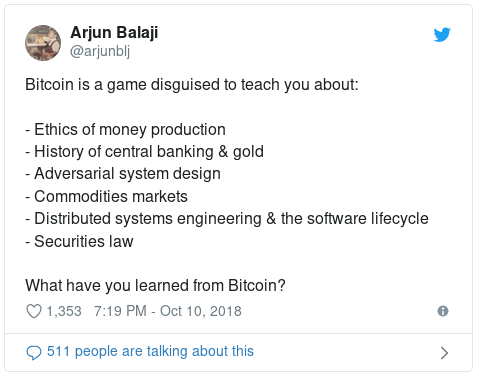
\includegraphics[width=7cm]{assets/images/the-tweet.png}
\end{center}

De \textit{21 lektioner} er struktureret i bundter af syv, hvilket resulterer i tre kapitler. Hvert kapitel betragter Bitcoin gennem en ny linse og uddrager, hvad man kan lære ved at inspicere dette mærkelige netværk fra en anden vinkel.\paragraph{\hyperref[ch:philosophy]{Kapitel 1}}{udforsker den filosofiske lære om Bitcoin. Samspillet mellem uforanderlighed og forandring, begrebet ægte knaphed, Bitcoins perfekte undfangelse, identitetsproblemet, modsigelsen mellem replikation og lokalitet, ytringsfrihedens kraft og grænserne for viden. }

\paragraph{\hyperref[ch:economics]{Kapitel 2}}{udforsker den økonomiske lære af Bitcoin. Disse lektioner omhandler finansiel uvidenhed, inflation, værdi, penge og pengenes historie, brøkreservebankvæsen og hvordan Bitcoin genindfører stabile penge på en snedig, indirekte måde.}

\paragraph{\hyperref[ch:technology]{Kapitel 3}}{udforsker nogle af de erfaringer, jeg har lært ved at undersøge teknologien i Bitcoin. Hvorfor der er styrke i tal, refleksioner over tillid, hvorfor det at fortælle tiden kræver arbejde, hvordan det at bevæge sig langsomt og ikke ødelægge ting er en egenskab og ikke en fejl, hvad Bitcoins skabelse kan fortælle os om privatliv, hvorfor cypherpunks skriver kode (og ikke love), og hvilke metaforer der kan være nyttige til at udforske Bitcoins fremtid.}

~

Hver lektion indeholder flere citater og links i teksten. Hvis en id\'e er værd at udforske nærmere, kan du følge linkene til relaterede værker i fodnoterne eller i bibliografien.

Selvom en vis forhåndsviden om Bitcoin er gavnlig, håber jeg, at disse lektioner kan fordøjes af enhver nysgerrig læser. Selvom nogle relaterer til hinanden, bør hver lektion kunne stå for sig selv og de kan læses uafhængigt af hinanden. Jeg har gjort mit bedste for at undgå teknisk jargon, selvom nogle domænespecifikke ord er uundgåelige.

Jeg håber, at mine tekster kan inspirere andre til at grave under overfladen og undersøge nogle af de dybere spørgsmål, som Bitcoin rejser. Min egen inspiration kom fra en lang række forfattere og indholdsskabere, hvem jeg er evigt taknemmelig.

Sidst, men ikke mindst: Mit mål med at skrive dette er ikke at overbevise dig om noget som helst. Mit mål er at få dig til at tænke og at vise dig, at der er meget mere ved Bitcoin, end man umiddelbart skulle tro. Jeg kan ikke engang fortælle dig, hvad Bitcoin er, eller hvad Bitcoin vil lære dig. Det bliver du nødt til selv at finde ud af.\begin{quotation}\begin{samepage}
\enquote{Herfra er der ingen vej tilbage. Du tager den blå pille - historien slutter, du vågner op i din seng og tror på, hvad du vil tro på. Du tager den røde pille\footnote{den \textit{orange} pille} --- du forbliver i Eventyrland, og jeg viser dig, hvor dybt kaninhullet når.}
\begin{flushright} -- Morpheus \end{flushright}\end{samepage}\end{quotation}

\begin{figure}
  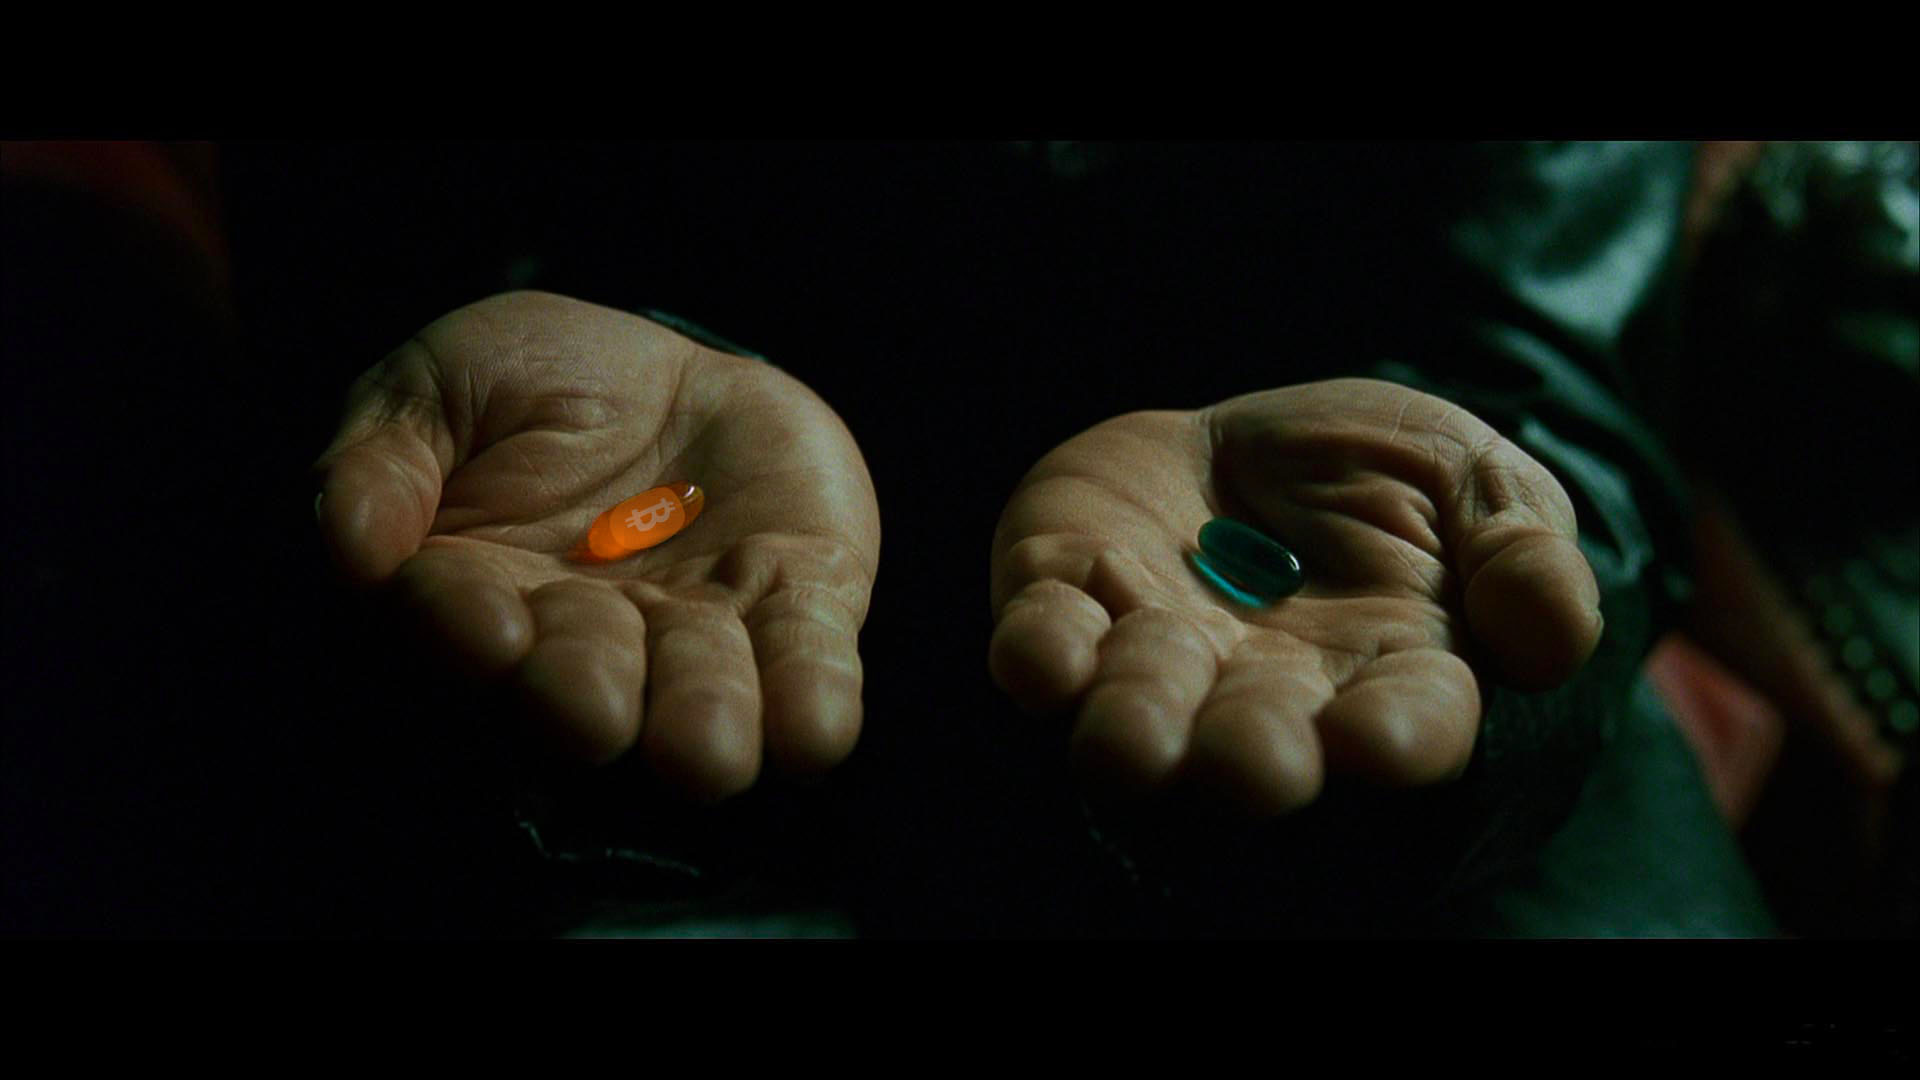
\includegraphics{assets/images/bitcoin-orange-pill.jpg}
  \caption*{Husk: Alt, hvad jeg tilbyder, er sandheden. Intet andet.}
  \label{fig:bitcoin-orange-pill}
\end{figure}%
% [Morpheus]: https://en.wikipedia.org/wiki/Red_pill_and_blue_pill#The_Matrix_(1999)
% [this question]: https://twitter.com/arjunblj/status/1050073234719293440
%
% <!-- Internal -->
% [chapter1]: {{ 'bitcoin/lessons/ch1-00-philosophy' | absolute_url }}
% [chapter2]: {{ 'bitcoin/lessons/ch2-00-economics' | absolute_url }}
% [chapter3]: {{ 'bitcoin/lessons/ch3-00-technology' | absolute_url }}
%
% <!-- Wikipedia -->
% [alice]: https://en.wikipedia.org/wiki/Alice%27s_Adventures_in_Wonderland
% [carroll]: https://en.wikipedia.org/wiki/Lewis_Carroll

\part{Filosofi}
\label{ch:philosophy}
\chapter*{Filosofi}

\begin{chapquote}{Lewis Carroll, \textit{Alice i Eventyrland}} Musen kiggede spørgende på hende. Det så ud, som om den blinkede med det ene af sine små øjne, men den sagde ikke noget. \end{chapquote}

Hvis man ser overfladisk på Bitcoin, kan man konkludere, at den er langsom, spild af ressourcer, unødvendigt redundant og overdrevent paranoid. Hvis man ser nysgerrigt på Bitcoin, finder man måske ud af, at tingene ikke er, som de ser ud ved første øjekast.

Bitcoin har det med at tage dine antagelser og vende dem på hovedet. Efter et stykke tid, lige når du er ved at finde dig til rette igen, bryder Bitcoin igennem muren som en elefant i en porcelænsbutik og knuser dine antagelser endnu en gang.\begin{figure}
  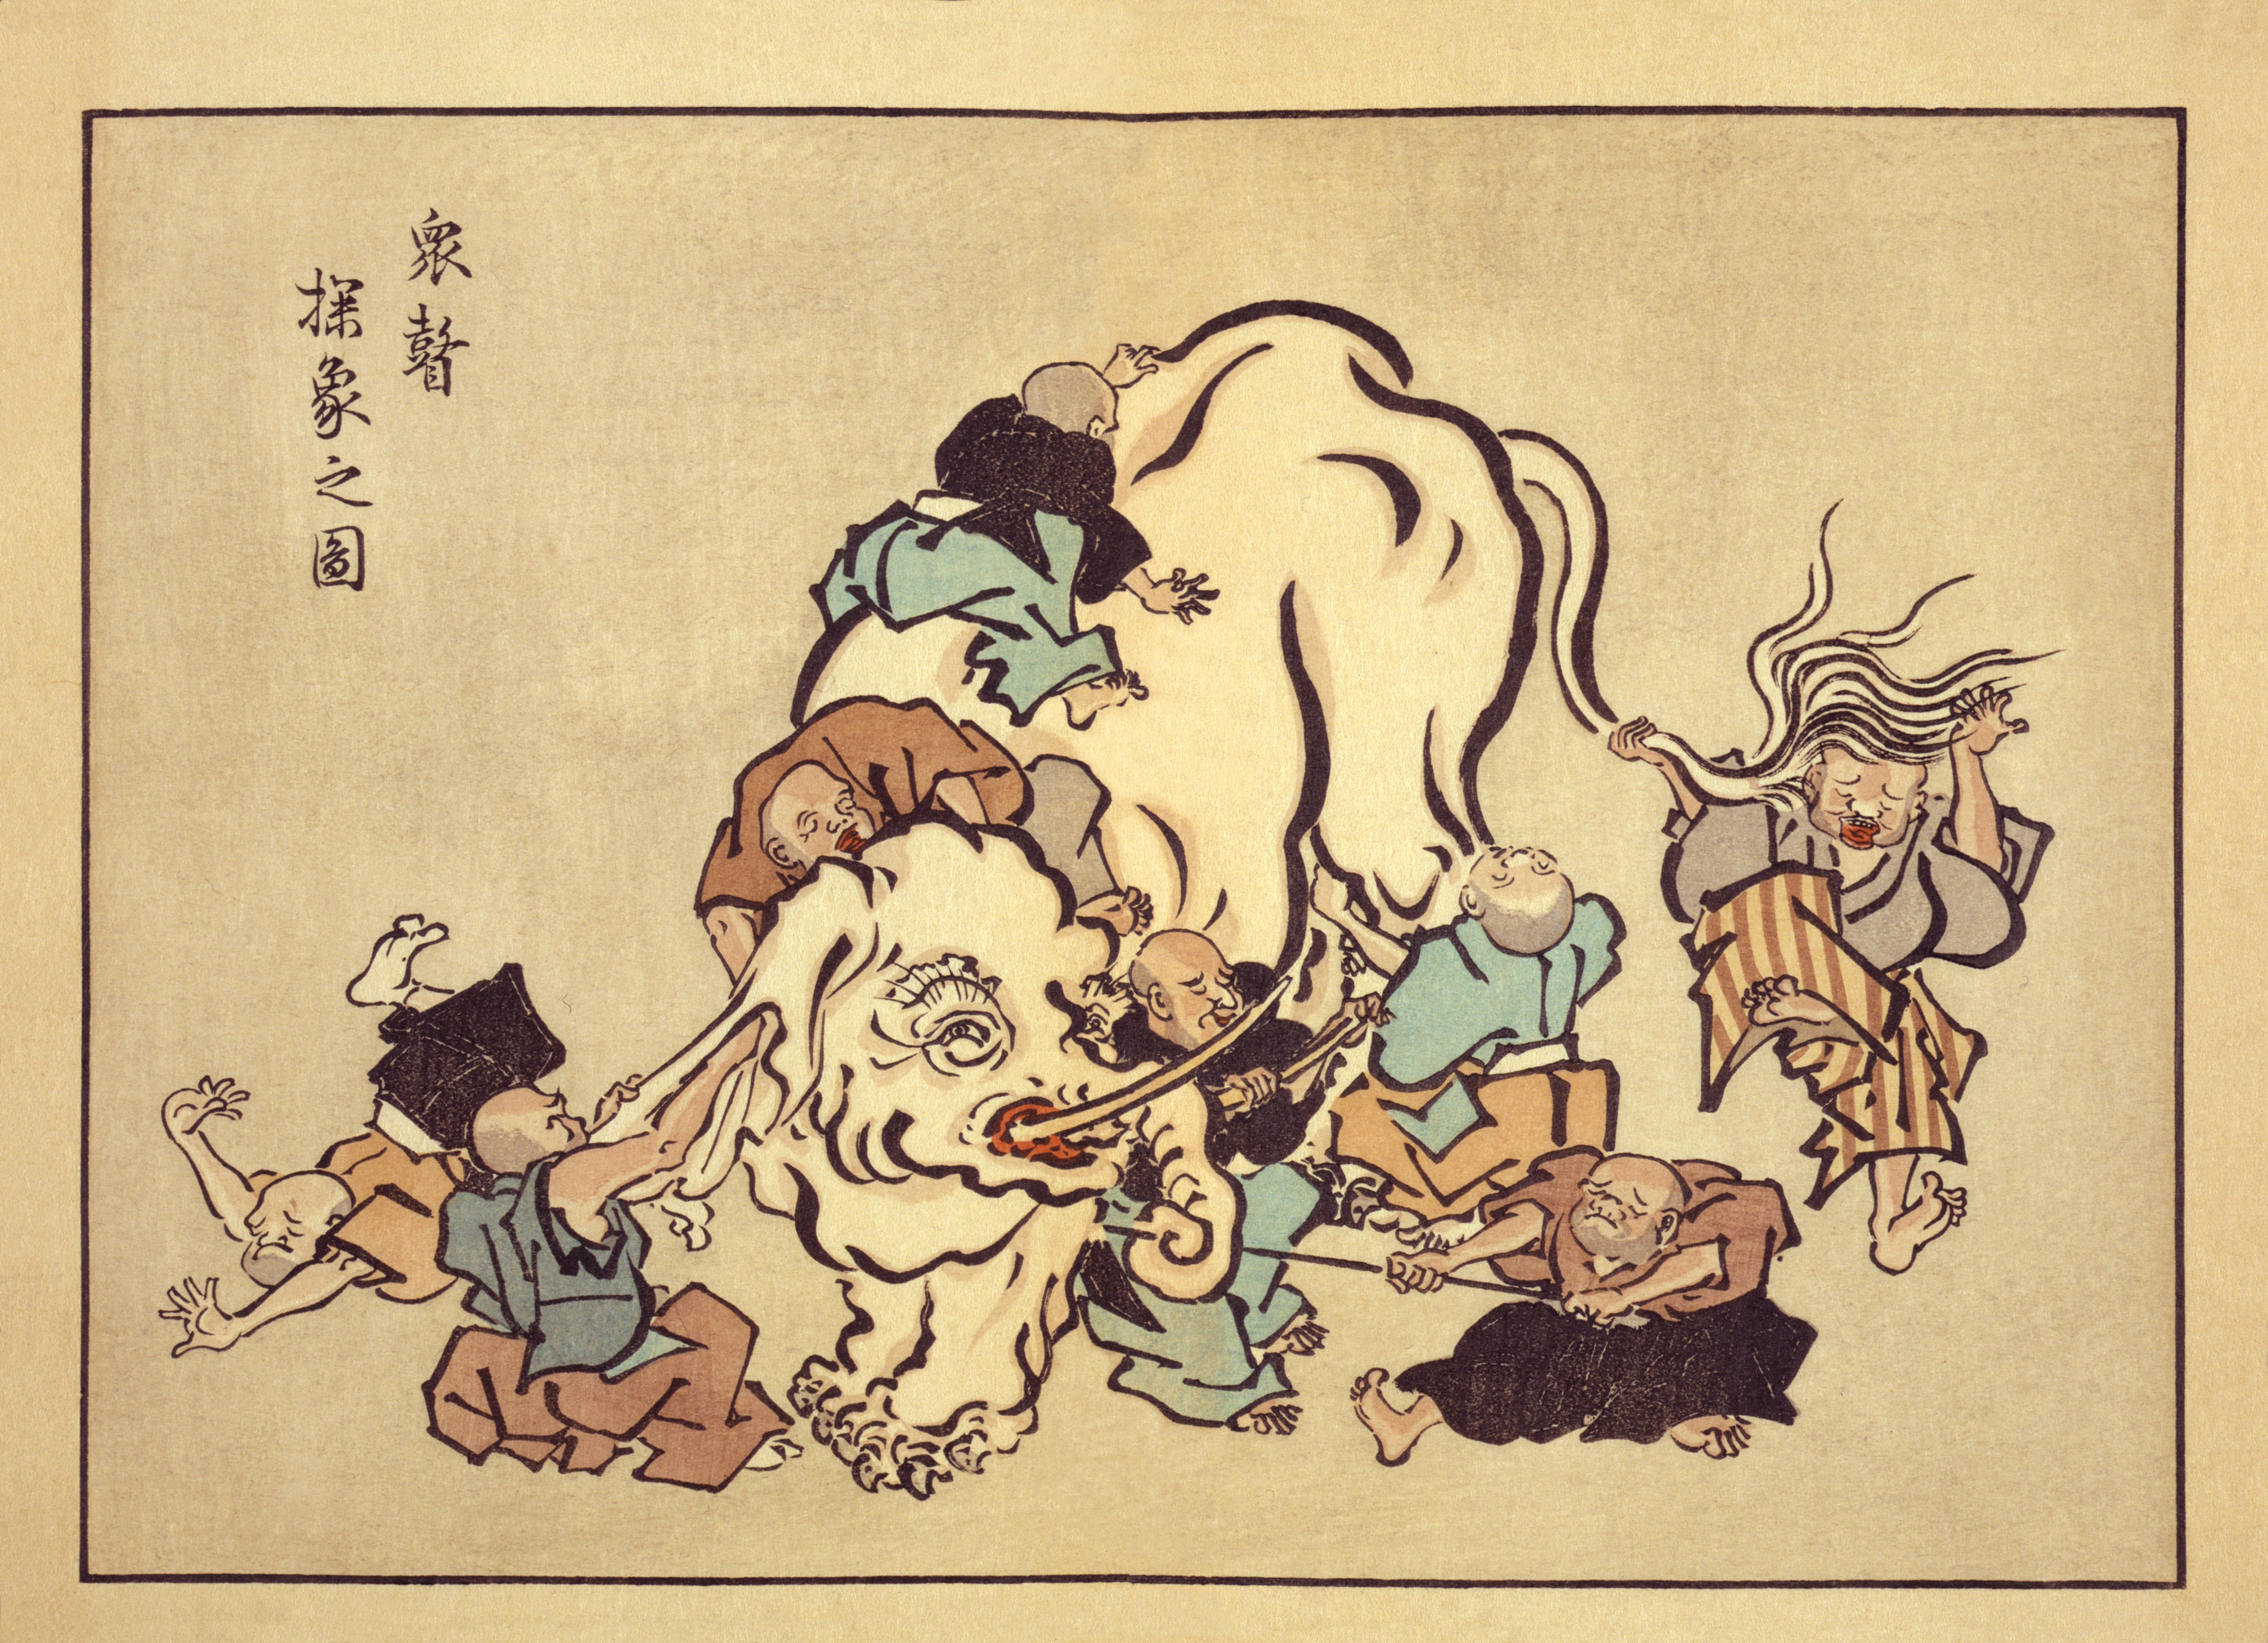
\includegraphics{assets/images/blind-monks.jpg}
  \caption{Blinde munke undersøger Bitcoin-elefanten}
  \label{fig:blind-monks}
\end{figure}

Bitcoin er et barn af mange discipliner. Som blinde munke, der undersøger en elefant, vil alle se denne nye teknologi fra sin egen vinkel. Og alle vil nå frem til forskellige konklusioner om dyrets natur.

De følgende lektioner handler om nogle af mine antagelser, som Bitcoin knuste, og de konklusioner, jeg nåede frem til. Filosofiske spørgsmål om uforanderlighed, knaphed, lokalitet og identitet bliver udforsket i de første fire lektioner. Hver del består af syv lektioner.

~\begin{samepage} Del~\ref{ch:philosophy} -- Filosofi:\begin{enumerate}
  \item Uforanderlighed og forandring \item Knaphedens knaphed \item Replikation og lokalitet \item Problemet med identitet \item En perfekt undfangelse \item Ytringsfrihedens kraft \item Grænserne for viden \end{enumerate}
\end{samepage}

Lektion \ref{les:5} udforsker hvordan Bitcoins oprindelseshistorie ikke bare er fascinerende, men også helt afgørende for et lederløst system. De sidste to lektioner i dette kapitel udforsker ytringsfrihedens kraft og grænserne for vores individuelle viden, hvilket afspejles af Bitcoin-kaninhullets overraskende dybde.

Jeg håber, at du vil finde Bitcoins verden lige så lærerig, fascinerende og underholdende, som jeg gjorde og stadig gør. Jeg inviterer dig til at følge den hvide kanin og udforske dybderne i dette kaninhul. Hold nu fast i dit lommeur, hop ned og nyd faldet. 
\chapter{Uforanderlighed og forandring}
\label{les:1}

\begin{chapquote}{Alice} \enquote{Mon jeg er blevet en anden i nattens løb? Vent nu lidt - var jeg den samme, da jeg stod op i morges? Jeg synes næsten, jeg kan huske, jeg var lidt anderledes. Men hvis ikke jeg var den samme, så er spørgsmålet jo: hvem i alverden er jeg da? Ja, det er det, der er så gådefuldt!} \end{chapquote}

Bitcoin er i sagens natur svær at beskrive. Det er en \textit{ny ting}, og ethvert forsøg på at drage en sammenligning med tidligere koncepter - om det så er ved at kalde det digitalt guld eller pengenes internet - vil utvivlsomt komme til kort. Uanset hvilken analogi du foretrækker, er der to aspekter af Bitcoin, som er helt essentielle: decentralisering og uforanderlighed.\paragraph{} En måde at tænke på Bitcoin er som en automatiseret social kontrakt\footnote{Hasu, Unpacking Bitcoin's Social Contract~\cite{social-contract}}. Softwaren er kun en brik i puslespillet, og at håbe på at ændre Bitcoin ved at ændre softwaren er en nytteløs øvelse. Man bliver nødt til at overbevise resten af netværket om at indføre ændringerne, hvilket mere er en psykologisk indsats end en softwareteknisk.\paragraph{} Det følgende vil måske lyde absurd i begyndelsen, som så mange andre ting på dette område, men ikke desto mindre tror jeg, at det er sandt: Du kan ikke ændre Bitcoin, men Bitcoin vil ændre dig.\begin{quotation}\begin{samepage} \enquote{Bitcoin vil ændre os mere, end vi vil ændre den.} \begin{flushright} -- Marty Bent\footnote{Tales From the Crypt~\cite{tftc21}}
\end{flushright}\end{samepage}\end{quotation}

Det tog mig lang tid at indse dybden af dette. Eftersom Bitcoin bare er software, og det hele er open source, kan man bare ændre tingene efter forgodtbefindende, ikke? Forkert. \textit{Meget} forkert. Det er ikke overraskende, at Bitcoins skaber fuldt ud var klar over dette.\begin{quotation}\begin{samepage} \enquote{Bitcoins natur er sådan, at da version 0.1 blev frigivet, blev kernedesignet mejslet i sten for resten af dens levetid.} \begin{flushright} -- Satoshi Nakamoto\footnote{BitcoinTalk forumindlæg: `Re: Transactions and Scripts\ldots'~\cite{satoshi-set-in-stone}}
\end{flushright}\end{samepage}\end{quotation}

Mange mennesker har forsøgt at ændre Bitcoins natur. Indtil videre har de alle fejlet. Mens der er et endeløst hav af forgreninger og altcoins (alternativer til Bitcoins), gør Bitcoin-netværket stadig sin ting, ligesom det gjorde, da det første knudepunkt gik online. Altcoins vil ikke have betydning i det lange løb. Forgreningerne vil til sidst uddø. Bitcoin er det eneste, der virkelig betyder noget. Så længe vores grundlæggende forståelse af matematik og/eller fysik ikke ændrer sig, vil Bitcoin fortsætte uden bekymringer.\begin{quotation}\begin{samepage}
\enquote{Bitcoin er det første eksempel på en ny livsform. Den lever og ånder på internettet. Den overlever, fordi den kan betale folk for at holde den i live. Den kan ikke ændres. Den kan ikke debatteres med. Den kan ikke pilles ved. Den kan ikke bestikkes. Den kan ikke stoppes. Hvis atomkrig ødelagde halvdelen af vores planet, ville den fortsætte med at leve ubeskadiget.}
\begin{flushright} -- Ralph Merkle\footnote{DAOs, Democracy and Governance,~\cite{merkle-dao}}
\end{flushright}\end{samepage}\end{quotation}

Bitcoin-netværkets hjerteslag vil overleve alle vores.

~

At indse ovenstående ændrede mig langt mere, end de tidligere blokke i Bitcoins blokkæde nogensinde vil gøre. Det ændrede min tidspræference, min forståelse af økonomi, mine politiske synspunkter og så meget mere. Den ændrer endda folks kostvaner.\footnote{Inside the World of the Bitcoin Carnivores,~\cite{carnivores}}. Hvis du synes, at alt dette virker skørt, er du i godt selskab. Alt dette er skørt, men alligevel sker det.

~\paragraph{Bitcoin har lært mig, at den ikke ændrer sig. Det gør jeg.}% ---
%
% #### Through the Looking-Glass
%
% - [Bitcoin's Gravity: How idea-value feedback loops are pulling people in][gravity]
% - [Lesson 18: Move slowly and don't break things][lesson18]
%
% #### Down the Rabbit Hole
%
% - [Unpacking Bitcoin's Social Contract][automated social contract]: A framework for skeptics by Hasu
% - [DAOs, Democracy and Governance][Ralph Merkle] by Ralph C. Merkle
% - [Marty's Bent][bent]: A daily newsletter highlighting signal in Bitcoin by Marty Bent
% - [Technical Discussion on Bitcoin's Transactions and Scripts][Satoshi Nakamoto] by Satoshi Nakamoto, Gavin Andresen, and others
% - [Inside the World of the Bitcoin Carnivores][carnivores]: Why a small community of Bitcoin users is eating meat exclusively by Jordan Pearson
% - [Tales From the Crypt][tftc] hosted by Marty Bent
%
% <!-- Internal -->
% [gravity]: 
% [lesson18]: {{ 'bitcoin/lessons/ch3-18-move-slowly-and-dont-break-things' | absolute_url }}
%
% <!-- Further Reading -->
% [automated social contract]: https://medium.com/@hasufly/bitcoins-social-contract-1f8b05ee24a9
% [carnivores]: https://motherboard.vice.com/en_us/article/ne74nw/inside-the-world-of-the-bitcoin-carnivores
% [tftc]: https://tftc.io/tales-from-the-crypt/
% [bent]: https://tftc.io/martys-bent/
%
% <!-- Quotes -->
% [Ralph Merkle]: http://merkle.com/papers/DAOdemocracyDraft.pdf
% [Satoshi Nakamoto]: https://bitcointalk.org/index.php?topic=195.msg1611#msg1611
%
% <!-- Twitter People -->
% [Marty Bent]: https://twitter.com/martybent
%
% <!-- Wikipedia -->
% [alice]: https://en.wikipedia.org/wiki/Alice%27s_Adventures_in_Wonderland
% [carroll]: https://en.wikipedia.org/wiki/Lewis_Carroll

\chapter{Knaphedens knaphed}
\label{les:2}

\begin{chapquote}{Alice}
\enquote{Det er mere end nok - jeg håber, jeg ikke vokser mere\ldots}
\end{chapquote}

Generelt synes den teknologiske udvikling at gøre ting mere tilgængelige. Flere og flere mennesker er i stand til at nyde, det, der tidligere har været luksusvarer. Snart vil vi alle leve som konger, hvilket de fleste af os allerede gør. Som Peter Diamandis skrev i \textit{Abundance}~\cite{abundance}: \enquote{Teknologi er en ressourcefrigørende mekanisme. Den kan forvandle det, som engang var knapt, til det, der nu er rigeligt.}

Bitcoin, som i sig selv er en avanceret teknologi, bryder med denne tendens og skaber en ny vare, som er virkelig knap. Der er endda nogle, der hævder, at det er en af de mest knappe ting i universet. Udbuddet af Bitcoins kan ikke øges, uanset hvor mange kræfter der anvendes på at skabe mere.\begin{quotation}\begin{samepage} \enquote{Kun to ting er virkelig knappe: tid og bitcoin.} \begin{flushright} -- Saifedean Ammous\footnote{Præsentation af Bitcoinstandarden~\cite{bitcoinstandard-pres}}
\end{flushright}\end{samepage}\end{quotation}

Paradoksalt nok gør den det ved hjælp af en kopieringsmekanisme. Transaktionerne sendes, blokkene distribueres, den distribuerede hovedbog (som er en logbog med alle transaktionerne) er - ja, du gættede det - distribueret. Alle disse ord betyder i virkeligheden bare kopiering. For pokker, Bitcoin kopierer endda sig selv til så mange computere som muligt ved at tilskynde individuelle mennesker til at køre fulde knudepunkter og udvinde nye blokke.

Alt det arbejde, der er med duplikering, er en vidunderlig, koordineret indsats for at skabe ægte knaphed.\paragraph{I en tid med overflod har Bitcoin lært mig, hvad reel knaphed er.}% ---
%
% #### Through the Looking-Glass
%
% - [Lesson 14: Sound money][lesson14]
%
% #### Down the Rabbit Hole
%
% - [The Bitcoin Standard: The Decentralized Alternative to Central Banking][bitcoin-standard]
% - [Abundance: The Future Is Better Than You Think][Abundance] by Peter Diamandis
% - [Presentation on The Bitcoin Standard][bitcoin-standard-presentation] by Saifedean Ammous
% - [Modeling Bitcoin's Value with Scarcity][planb-scarcity] by PlanB
% - 🎧 [Misir Mahmudov on the Scarcity of Time & Bitcoin][tftc60] TFTC #60 hosted by Marty Bent
% - 🎧 [PlanB – Modelling Bitcoin's digital scarcity through stock-to-flow techniques][slp67] SLP #67 hosted by Stephan Livera
%
% <!-- Through the Looking-Glass -->
% [lesson14]: {{ 'bitcoin/lessons/ch2-14-sound-money' | absolute_url }}
%
% <!-- Down the Rabbit Hole -->
% [Abundance]: https://www.diamandis.com/abundance
% [bitcoin-standard]: http://amzn.to/2L95bJW
% [bitcoin-standard-presentation]: https://www.bayernlb.de/internet/media/de/ir/downloads_1/bayernlb_research/sonderpublikationen_1/bitcoin_munich_may_28.pdf
% [planb-scarcity]: https://medium.com/@100trillionUSD/modeling-bitcoins-value-with-scarcity-91fa0fc03e25
% [tftc60]: https://anchor.fm/tales-from-the-crypt/episodes/Tales-from-the-Crypt-60-Misir-Mahmudov-e3aibh
% [slp67]: https://stephanlivera.com/episode/67
%
% <!-- Wikipedia -->
% [alice]: https://en.wikipedia.org/wiki/Alice%27s_Adventures_in_Wonderland
% [carroll]: https://en.wikipedia.org/wiki/Lewis_Carroll

\chapter{Replikation og lokalitet}
\label{les:3}

\begin{chapquote}{Lewis Carroll, \textit{Alice i Eventyrland}} Så kom der en vred stemme - kaninens - \enquote{Pat, Pat! Hvor er du?} \end{chapquote}

Bortset fra kvantemekanik er lokalitet ikke et problem i den fysiske verden. Spørgsmålet \textit{\enquote{Hvor er X?}} kan let besvares, uanset om X er en person eller et objekt. I den digitale verden er spørgsmålet om \textit{hvor} allerede et vanskeligt spørgsmål, men ikke umuligt at besvare. Hvor er dine e-mails egentlig? Et dårligt svar ville være \enquote{skyen}, som bare er en andens computer. Men hvis du ønskede finde alle de harddiske, som dine e-mails er gemt på, kunne du i teorien finde dem.

Med bitcoin er spørgsmålet om \enquote{hvor} \textit{virkelig} vanskeligt. Hvor er dine bitcoins helt præcist?\begin{quotation}\begin{samepage} \enquote{Jeg åbnede øjnene, så mig omkring og stillede det uundgåelige, traditionelle, beklageligt overbrugte spørgsmål, der stilles efter en operation: `Hvor er jeg?'} \begin{flushright} -- Daniel Dennett\footnote{Daniel Dennett, \textit{Where Am I?}~\cite{where-am-i}}
\end{flushright}\end{samepage}\end{quotation}

Problemet er todelt: For det første er den distribuerede hovedbog distribueret gennem fuld replikation, hvilket betyder, at hovedbogen er overalt. For det andet er der ingen bitcoins. Hverken fysisk eller \textit{teknisk}.

Bitcoin holder styr på et sæt ubrugte transaktionsoutputs uden nogensinde at skulle henvise til en enhed, der repræsenterer en bitcoin. Eksistensen af \'en bitcoin udledes ved at se på mængden af ubrugte transaktionsoutputs og gennemgå alle tidligere overførsler, hvor summen af alle overførelser giver 100 millioner satoshis, som er basisenheden for en bitcoin.\begin{quotation}\begin{samepage} \enquote{Hvor er de på nuværende tidspunkt i transit? \href{...}{} For det første er der ingen bitcoins. De eksisterer simpelthen ikke. De eksisterer ikke. Der er hovedbogsposter i en hovedbog, der er delt \href{...}{} De findes ikke på noget fysisk sted. Hovedbogen findes stort set på alle fysiske steder. Geografi giver ikke mening - det vil ikke hjælpe dig med at forstå din politik her.} \begin{flushright} -- Peter Van Valkenburgh\footnote{Peter Van Valkenburgh i podcasten \textit{What Bitcoin Did}, episode 49 \cite{wbd049}}
\end{flushright}\end{samepage}\end{quotation}

Så hvad ejer du egentlig, når du siger \textit{\enquote{Jeg har en bitcoin}}, hvis der ikke findes nogen bitcoins? Kan du huske alle de mærkelige ord, som du blev tvunget til at skrive ned af din bitcoin-tegnebog? Det viser sig, at disse magiske ord er, hvad du ejer: en trylleformular\footnote{The Magic Dust of Cryptography: How digital information is changing our society \cite{gigi:magic-spell}} som kan bruges til at tilføje poster til den offentlige hovedbog - nøglerne til at \enquote{flytte} nogle bitcoins. Det er derfor, at dine private nøgler i praksis \textit{er} dine bitcoins. Hvis du tror, at jeg finder på alt det her, er du velkommen til at sende mig dine private nøgler.\paragraph{Bitcoin har lært mig, at lokalitet er en vanskelig størrelse.}% ---
%
% #### Through the Looking-Glass
%
% - [The Magic Dust of Cryptography: How digital information is changing our society][a magic spell]
%
% #### Down the Rabbit Hole
%
% - [Where Am I?][Daniel Dennett] by Daniel Dennett
% - 🎧 [Peter Van Valkenburg on Preserving the Freedom to Innovate with Public Blockchains][wbd049] WBD #49 hosted by Peter McCormack
%
% <!-- Through the Looking-Glass -->
% [a magic spell]: 
%
% <!-- Down the Rabbit Hole -->
% [Daniel Dennett]: https://www.lehigh.edu/~mhb0/Dennett-WhereAmI.pdf
% [1st Amendment]: https://en.wikipedia.org/wiki/First_Amendment_to_the_United_States_Constitution
% [wbd049]: https://www.whatbitcoindid.com/podcast/coin-centers-peter-van-valkenburg-on-preserving-the-freedom-to-innovate-with-public-blockchains
%
% <!-- Wikipedia -->
% [alice]: https://en.wikipedia.org/wiki/Alice%27s_Adventures_in_Wonderland
% [carroll]: https://en.wikipedia.org/wiki/Lewis_Carroll

\chapter{Problemet med identitet}
\label{les:4}

\begin{chapquote}{Lewis Carroll, \textit{Alice i Eventyrland}} \enquote{Hvem er du?} spurgte larven. \end{chapquote}

Nic Carter har i en hyldest til Thomas Nagels behandling af det samme spørgsmål, i forbindelse med en flagermus, skrevet en fremragende artikel, der diskuterer følgende spørgsmål: Hvordan er det at være en bitcoin? Han viser på glimrende vis, at åbne, offentlige blokkæder i almindelighed og Bitcoin i særdeleshed lider under den samme gåde som Theseus' skib\footnote{I identitetens metafysik er Theseus' skib et tankeeksperiment, der rejser spørgsmålet om, hvorvidt et objekt, der har fået udskiftet alle sine komponenter, grundlæggende forbliver det samme objekt.~\cite{wiki:theseus}}: Hvilken Bitcoin er den rigtige Bitcoin?\begin{quotation}\begin{samepage} \enquote{Overvej, hvor lidt Bitcoins komponenter forbliver de samme. Hele kodebasen er blevet omskrevet, ændret og udvidet, så den knap nok ligner sin oprindelige version. \href{...}{} Registreringen af, hvem der ejer hvad, selve hovedbogen, er stort set netværkets eneste vedvarende træk \href{...}{} For at blive betragtet som virkelig lederløs, skal du opgive den nemme løsning det er, at have \'en computer, der kan udpege den \textit{rigtige} blokkæde som den legitime.} \begin{flushright} -- Nic Carter\footnote{Nic Carter, \textit{What is it like to be a bitcoin?} \cite{bitcoin-identity}}
\end{flushright}\end{samepage}\end{quotation}

Det ser ud til, at teknologiens fremskridt fortsætter med at tvinge os til at tage disse filosofiske spørgsmål alvorligt. Før eller senere vil selvkørende biler blive konfronteret med virkelige versioner af \enquote{sporvognsproblemet}, hvor de bliver tvunget til at træffe etiske beslutninger om, hvilke liv der betyder noget, og hvilke der ikke gør.

Kryptovalutaer, især siden den første omstridte hårde-forgrening, tvinger os til at tænke over og blive enige om identitetens metafysik. Det er interessant, at de to største eksempler, vi hidtil har set, har ført til to forskellige svar. Den 1. august 2017 delte Bitcoin sig i to lejre. Markedet besluttede, at den uændrede kæde er den originale Bitcoin. Et år tidligere, den 25. oktober 2016, delte Ethereum sig i to lejre. Markedet besluttede, at den \textit{ændrede} kæde er den oprindelige Ethereum.

Hvis fuldt decentraliseret, vil spørgsmålene stillet af \textit{Theseus' skib} skulle besvares igen og igen, så længe disse netværk af værdioverførsel eksisterer.\paragraph{Bitcoin har lært mig, at decentralisering er i modstrid med identitet.}% ---
%
% #### Down the Rabbit Hole
%
% - [What Is It Like to be a Bat?][in regards to a bat] by Thomas Nagel
% - [What is it like to be a bitcoin?] by Nic Carter
% - [Ship of Theseus], [trolley problem] on Wikipedia
%
% [in regards to a bat]: https://en.wikipedia.org/wiki/What_Is_it_Like_to_Be_a_Bat%3F
% [What is it like to be a bitcoin?]: https://medium.com/s/story/what-is-it-like-to-be-a-bitcoin-56109f3e6753
% [Ship of Theseus]: https://en.wikipedia.org/wiki/Ship_of_Theseus
% [trolley problem]: https://en.wikipedia.org/wiki/Trolley_problem
%
% <!-- Wikipedia -->
% [alice]: https://en.wikipedia.org/wiki/Alice%27s_Adventures_in_Wonderland
% [carroll]: https://en.wikipedia.org/wiki/Lewis_Carroll

\chapter{En perfekt undfangelse}
\label{les:5}

\begin{chapquote}{Lewis Carroll, \textit{Alice i Eventyrland}} \enquote{Deres hoveder er væk,} råbte soldaterne som svar.\ldots
\end{chapquote}

Alle elsker en god oprindelseshistorie. Bitcoins oprindelseshistorie er fascinerende, og detaljerne i den er vigtigere, end man umiddelbart skulle tro. Hvem er Satoshi Nakamoto? Var han \'en person eller en gruppe mennesker? Var han en kvinde? Et tidsrejsende rumvæsen eller en avanceret kunstig intelligens? Hvis vi ser bort fra de besynderlige teorier, vil vi nok aldrig finde ud af det. Og det er vigtigt.

Satoshi valgte at være anonym. Han plantede frøet til Bitcoin. Han blev hængende længe nok til at sikre, at netværket ikke døde i sin barndom. Og så forsvandt han.

Det som kan se ud som et underligt anonymitetsstunt, er faktisk afgørende for et ægte decentraliseret system. Der er ingen centraliseret kontrol, ingen centraliseret autoritet og ingen opfinder. Ingen at retsforfølge, torturere, afpresse eller udnytte. Det er en perfekt undfangelse af teknologi.\begin{quotation}\begin{samepage} \enquote{En af de største ting, Satoshi gjorde, var at forsvinde.} \begin{flushright} -- Jimmy Song\footnote{Jimmy Song, \textit{Why Bitcoin is Different}. \cite{bitcoin-different}}
\end{flushright}\end{samepage}\end{quotation}

\newpage

Siden Bitcoins fødsel er der blevet skabt tusindvis af andre kryptovalutaer. Ingen af disse kloner deler dens oprindelseshistorie. Hvis du vil erstatte Bitcoin, bliver du nødt til at overgå dens oprindelseshistorie. Ideernes overlevelse dikteres af de fortællinger, som spredes.\begin{quotation}\begin{samepage} \enquote{Guld blev først formet til smykker og brugt til byttehandel for mere end 7.000 år siden. Guldets fængslende glans førte til, at det blev betragtet som en gave fra guderne.} \begin{flushright} Münze Österreich\footnote{Münze Österreich, \textit{Gold: The Extraordinary Metal} \cite{gold-gift-gods}}
\end{flushright}\end{samepage}\end{quotation}

Ligesom guld i oldtiden, kan Bitcoin betragtes som en gave fra guderne. I modsætning til guld er Bitcoins oprindelse udelukkende menneskelig. Og denne gang ved vi, hvem guderne bag udvikling og vedligeholdelse er: mennesker over hele verden, anonyme eller ej.\paragraph{Bitcoin har lært mig, at fortællinger er vigtige.}% ---
%
% #### Down the Rabbit Hole
%
% - [Why Bitcoin is different][Jimmy Song] by Jimmy Song
% - [Gold: The Extraordinary Metal] by the Austrian Mint
%
% <!-- Down the Rabbit Hole -->
% [Jimmy Song]: https://medium.com/@jimmysong/why-bitcoin-is-different-e17b813fd947
% [Gold: The Extraordinary Metal]: https://www.muenzeoesterreich.at/eng/discover/for-investors/gold-the-extraordinary-metal
%
% <!-- Wikipedia -->
% [alice]: https://en.wikipedia.org/wiki/Alice%27s_Adventures_in_Wonderland
% [carroll]: https://en.wikipedia.org/wiki/Lewis_Carroll

\chapter{Ytringsfrihedens kraft}
\label{les:6}

\begin{chapquote}{Lewis Carroll, \textit{Alice i Eventyrland}} \enquote{Undskyld?} sagde musen og rynkede panden, men meget høfligt, \enquote{talte du?} \end{chapquote}

Bitcoin er en id\'e. En id\'e, som i sin nuværende form er manifestationen af et maskineri, der udelukkende drives af tekst. Alle aspekter af Bitcoin er tekst: Hvidbogen (whitepaper) er tekst. Softwaren, som køres af knudepunkterne, er tekst. Hovedbogen er tekst. Transaktioner er tekst. Offentlige og private nøgler er tekst. Alle aspekter af Bitcoin er tekst og svarer dermed til ytring.\begin{quotation}\begin{samepage} \enquote{Kongressen må ikke vedtage nogen lov, der vedrører oprettelsen af en religion, eller forbud mod dens frie udøvelse; eller indskrænker ytringsfriheden, eller pressens frihed, eller folks ret til fredeligt at samles og at anmode staten om at få klagemål behandlet.} \begin{flushright} -- Første tilføjelse til USA's forfatning \end{flushright}\end{samepage}\end{quotation}

Selvom det sidste slag i kryptokrigen\footnote{\textit{Kryptokrigen} er et uofficielt navn for USA's og dets allieredes forsøg på at underminere kryptering.~\cite{eff-cryptowars}~\cite{wiki:cryptowars}} ikke er blevet udkæmpet endnu, vil det være meget svært at kriminalisere en id\'e, især en der er baseret på udveksling af tekstbeskeder. Hver gang en stat forsøger at forbyde tekst eller tale, glider vi ned ad en absurd sti, som uundgåeligt fører til vederstyggeligheder såsom ulovlige tal\footnote{Et ulovligt tal er et tal, der repræsenterer information, som er ulovlig at besidde, fremsige, formidle eller på anden måde overføre i visse jurisdiktioner.\cite{wiki:illegal-number}} og ulovlige primtal\footnote{Et ulovligt primtal er et tal, der repræsenterer information, hvis besiddelse eller distribution er forbudt i visse jurisdiktioner. Et af de første ulovlige primtal blev fundet i 2001. Når det fortolkes på en bestemt måde, beskriver det et computerprogram, der omgår det digitale rettighedsstyringssystem, der bruges på DVD'er. Distribution af et sådant program i USA er ulovligt i henhold til Digital Millennium Copyright Act. Et ulovligt primtal er en form for ulovligt tal.\cite{wiki:illegal-prime}}.

Så længe der er en del af verden, hvor tale er fri som i \textit{frihed}, er Bitcoin ustoppelig.\begin{quotation}\begin{samepage} \enquote{Der er ikke noget tidspunkt i en Bitcoin-transaktion, hvor Bitcoin ophører med at være \textit{tekst}. Det er \textit{altid tekst}, hele tiden. \href{...}{} Bitcoin er \textit{tekst}. Bitcoin er \textit{tale}. Det kan ikke reguleres i et frit land som USA med umistelige garanterede rettigheder og en \textit{første forfatningstilføjelse}, der udtrykkeligt udelukker udgivelseshandlinger fra statsligt tilsyn.} \begin{flushright} -- Beautyon\footnote{Beautyon, \textit{Why America can't regulate Bitcoin} \cite{america-regulate-bitcoin}}
\end{flushright}\end{samepage}\end{quotation}

\paragraph{Bitcoin har lært mig, at ytringsfrihed og fri software er ustoppelige i et frit samfund.}% ---
%
% #### Through the Looking-Glass
%
% - [The Magic Dust of Cryptography: How digital information is changing our society][a magic spell]
%
% #### Down the Rabbit Hole
%
% - [Why America can't regulate Bitcoin][Beautyon] by Beautyon
% - [First Amendment to the United States Constitution][1st Amendment], [Crypto Wars], [illegal numbers], [illegal primes] on Wikipedia
%
% <!-- Through the Looking-Glass -->
% [a magic spell]: 
%
% <!-- Down the Rabbit Hole -->
% [1st Amendment]: https://en.wikipedia.org/wiki/First_Amendment_to_the_United_States_Constitution
% [Crypto Wars]: https://en.wikipedia.org/wiki/Crypto_Wars
% [illegal numbers]: https://en.wikipedia.org/wiki/Illegal_number
% [illegal primes]: https://en.wikipedia.org/wiki/Illegal_prime
% [Beautyon]: https://hackernoon.com/why-america-cant-regulate-bitcoin-8c77cee8d794
%
% <!-- Wikipedia -->
% [alice]: https://en.wikipedia.org/wiki/Alice%27s_Adventures_in_Wonderland
% [carroll]: https://en.wikipedia.org/wiki/Lewis_Carroll

\chapter{Grænserne for viden}
\label{les:7}

\begin{chapquote}{Lewis Carroll, \textit{Alice i Eventyrland}} \enquote{Ned, ned, ned. Ville faldet aldrig få en ende?} \end{chapquote}

At begynde at arbejde med Bitcoin er en ydmygende oplevelse. Jeg troede, at jeg vidste ting. Jeg troede, at jeg var veluddannet. Jeg troede, at jeg i det mindste kunne min datalogi. Jeg har studeret det i årevis, så jeg burde da vide alt om digitale signaturer, hashfunktioner, kryptering, driftssikkerhed og netværk, ikke sandt?\paragraph{} Forkert.\paragraph{} Det er svært at lære alle de grundlæggende elementer, der får Bitcoin til at virke. At forstå dem alle i dybden er på grænsen til det umulige.\begin{quotation}\begin{samepage} \enquote{Ingen har fundet bunden af Bitcoin-kaninhullet.} \begin{flushright} -- Jameson Lopp\footnote{Jameson Lopp, tweet fra 11. november 2018 \cite{lopp-tweet}}
\end{flushright}\end{samepage}\end{quotation}

\begin{figure}
  \centering
  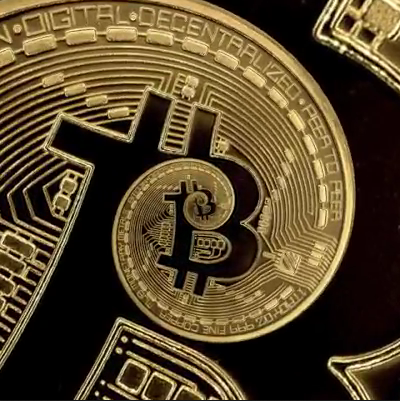
\includegraphics[width=7cm]{assets/images/rabbit-hole-bottomless.png}
  \caption{Bitcoin-kaninhullet er bundløst.}
  \label{fig:rabbit-hole-bottomless}
\end{figure}

Min liste over bøger, jeg skal læse, bliver ved med at vokse hurtigere, end jeg kan nå at læse dem. Listen over aviser og artikler, der skal læses, er næsten uendelig. Der er flere podcasts om alle disse emner, end jeg nogensinde ville kunne nå at lytte til. Det er virkelig overvældende. Desuden udvikler Bitcoin sig, og det er næsten umuligt at holde sig ajour med den accelererende innovationshastighed. Støvet fra det første lag har ikke engang lagt sig endnu, og folk har allerede bygget det andet lag og arbejder på det tredje.\paragraph{Bitcoin har lært mig, at jeg ved meget lidt om næsten alt. Den har lært mig, at dette kaninhul er bundløst.}% ---
%
% #### Down the Rabbit Hole
%
% - [Bitcoin Literature] by the Satoshi Nakamoto Institute
% - [Bitcoin Information & Resources][lopp-resources] by Jameson Lopp
% - [Educational Resources][bitcoin-only] by Bitcoin Only
%
% <!-- Twitter -->
% [Jameson Lopp]: https://twitter.com/lopp/status/1061415918616698881
%
% <!-- Down the Rabbit Hole -->
% [lopp-resources]: https://www.lopp.net/bitcoin-information.html
% [bitcoin-only]: https://bitcoin-only.com/#learning
% [Bitcoin Literature]: https://nakamotoinstitute.org/literature/
%
% <!-- Wikipedia -->
% [alice]: https://en.wikipedia.org/wiki/Alice%27s_Adventures_in_Wonderland
% [carroll]: https://en.wikipedia.org/wiki/Lewis_Carroll

\part{Økonomi}
\label{ch:economics}
\chapter*{Økonomi}

\begin{chapquote}{Lewis Carroll, \textit{Alice i Eventyrland}}
\enquote{Der stod et stort rosentræ nær indgangen til haven. Roserne på det var hvide, men tre gartnere var ivrigt i færd med at male dem røde. Alice syntes, at det så mærkeligt ud\ldots}
\end{chapquote}

Penge vokser ikke på træerne. Det er tåbeligt at tro, at de gør det, og vores forældre sørger for, at vi ved det, ved at gentage dette ordsprog som et mantra. Vi bliver opfordret til at bruge penge fornuftigt, til ikke at bruge dem letsindigt, og til at spare dem op i gode tider, så de kan hjælpe os gennem de dårlige. Penge vokser trods alt ikke på træerne.

Bitcoin har lært mig mere om penge, end jeg nogensinde troede, jeg ville få brug for at vide. Gennem den blev jeg tvunget til at udforske pengenes historie, bankvæsenet, forskellige økonomiske skoler og mange andre emner. Min søgen efter at forstå Bitcoin førte mig ned ad et væld af stier, hvoraf jeg forsøger at udforske nogle i dette kapitel.

I de første syv lektioner blev nogle af de filosofiske spørgsmål, som Bitcoin berører, diskuteret. De næste syv lektioner vil undersøge penge og økonomi nærmere.

~\begin{samepage} Del~\ref{ch:economics} -- Økonomi:\begin{enumerate}
  \setcounter{enumi}{7}
  \item Økonomisk uvidenhed \item Inflation \item Værdi \item Penge \item Pengenes historie og undergang \item Vanviddet i brøkreserve-bankvæsenet \item Stabile penge \end{enumerate}
\end{samepage}

Igen vil jeg kun være i stand til at kradse i overfladen. Bitcoin er ikke bare ambitiøst, men også bredt og dybt, hvilket gør det umuligt at dække alle relevante emner i en enkelt lektion, essay, artikel eller bog. Jeg tvivler på, at det overhovedet er muligt.

Bitcoin er en ny form for penge, hvilket gør det afgørende at lære om økonomi for at forstå den. Økonomi handler om menneskelige handlinger og samspillet mellem økonomiske aktører, og det er sandsynligvis en af de største og mest uklare brikker i Bitcoin-puslespillet.

Igen er disse lektioner en udforskning af de forskellige ting, jeg har lært af Bitcoin. De er en personlig afspejling af min rejse ned i kaninhullet. Da jeg ikke har nogen økonomisk baggrund, er jeg helt sikkert uden for min komfortzone og klar over, at enhver forståelse, jeg måtte have, er ufuldstændig. Jeg vil gøre mit bedste for at skitsere, hvad jeg har lært, selv med risiko for at gøre mig selv til grin. Når alt kommer til alt, forsøger jeg stadig at besvare spørgsmålet: \textit{\enquote{Hvad har du lært af Bitcoin?}}

Efter syv lektioner set gennem filosofiens briller, lad os bruge økonomiens briller til at se på syv mere. En tur på økonomiklasse er alt, hvad jeg kan tilbyde denne gang. Slutdestination: \textit{stabile penge}% [the question]: https://twitter.com/arjunblj/status/1050073234719293440
.

\chapter{Finansiel uvidenhed}
\label{les:8}

\begin{chapquote}{Lewis Carroll, \textit{Alice i Eventyrland}} \enquote{\enquote{Og hun vil sikkert synes, jeg er en dum lille pige! Nej, jeg vil ikke spørge om det. Jeg kan måske læse navnet et eller andet sted.}} \end{chapquote}

En af de mest overraskende ting for mig var den mængde af finans, økonomi og psykologi, der kræves for at få en forståelse af, hvad der ved første øjekast ser ud til at være et rent \textit{teknisk} system - et computernetværk. Som en lille fyr med behårede fødder sagde: \enquote{Det er en farlig forretning, Frodo, at træde ind i Bitcoin-verdenen. Du læser hvidbogen, og hvis du ikke holder dig på måtten, er det ikke til at vide, hvor du bliver ført hen.}

For at forstå et nyt monetært system, er man nødt til at kende det gamle. Jeg begyndte meget hurtigt at indse, at den mængde finansiel uddannelse, jeg havde fået i uddannelsessystemet, stort set var \textit{nul}.\paragraph{} Som femårig begyndte jeg at stille mig selv en masse spørgsmål: Hvordan fungerer banksystemet? Hvordan fungerer aktiemarkedet? Hvad er fiat-penge? Hvad er \textit{almindelige} penge? Hvorfor er der så megen gæld?\footnote{\url{https://www.usdebtclock.org/}} Hvor mange penge bliver der egentlig trykt, og hvem bestemmer det?\newpage

Efter en mild panik over omfanget af min uvidenhed, fandt jeg tryghed i at indse, at jeg var i godt selskab.\begin{quotation}\begin{samepage}
\enquote{Er det ikke ironisk, at Bitcoin har lært mig mere om penge end alle de år, jeg har brugt på at arbejde for finansielle institutioner? \ldots herunder, da jeg startede min karriere i en centralbank}
\begin{flushright} -- Aaron\footnote{Aaron (\texttt{@aarontaycc}, \texttt{@fiatminimalist}), tweet fra 12. december 2018~\cite{aarontaycc-tweet}}
\end{flushright}\end{samepage}\end{quotation}

\begin{quotation}\begin{samepage} \enquote{Jeg har lært mere om finans, økonomi, teknologi, kryptografi, menneskelig psykologi, politik, spilteori, lovgivning og mig selv i de sidste tre måneder med krypto, end jeg har i de sidste tre et halvt år på universitetet} \begin{flushright} -- Dunny\footnote{Dunny (\texttt{@BitcoinDunny}), tweet fra 28. november 2017~\cite{bitcoindunny-tweet}}
\end{flushright}\end{samepage}\end{quotation}

Dette er blot to af de mange bekendelser, der florerer på Twitter.\footnote{Se \url{http://bit.ly/btc-learned} for flere bekendelser på Twitter.} Bitcoin, som blev udforsket i Lektion  \ref{les:1}, er en levende ting. Mises hævdede, at økonomi også er en levende ting. Og som vi alle ved fra personlig erfaring, er levende ting i sagens natur svære at forstå.\begin{quotation}\begin{samepage} \enquote{Et videnskabeligt system er blot en station i en endeløs søgen efter viden. Det er nødvendigvis påvirket af den utilstrækkelighed, der ligger i enhver menneskelig indsats. Men at anerkende disse fakta betyder ikke, at nutidens økonomi er bagud. Det betyder blot, at økonomi er et levende væsen - og at leve indebærer både ufuldkommenhed og forandring.} \begin{flushright} -- Ludwig von Mises\footnote{Ludwig von Mises, \textit{Human Action} \cite{human-action}}
\end{flushright}\end{samepage}\end{quotation}

\newpage

Vi læser alle om forskellige finanskriser i nyhederne, og undrer os over, hvordan disse store redningspakker fungerer. Vi er forundrede over, at ingen nogensinde synes at blive stillet til ansvar for skader, der løber op i billioner. Jeg er stadig forundret, men i det mindste er jeg begyndt at få et indblik i, hvad der foregår i finansverdenen.

Nogle mennesker går endda så langt, at de tilskriver den generelle uvidenhed om disse emner til systemisk, bevidst uvidenhed. Mens historie, fysik, biologi, matematik og sprog alle er en del af vores uddannelse, bliver verdenen inden for penge og økonomi overraskende nok kun udforsket overfladisk, hvis overhovedet. Jeg spekulerer på, om folk stadig ville være villige til at optage så meget gæld, som de gør i øjeblikket, hvis alle blev uddannet i privatøkonomi og i, hvordan penge og gæld fungerer. Og så spekulerer jeg på, hvor mange lag aluminium der skal til for at lave en effektiv sølvpapirshat. Sandsynligvis tre.\begin{quotation}\begin{samepage} \enquote{Disse nedbrud og redningspakker er ikke tilfældigheder. Og det er heller ikke et uheld, at der ikke er nogen finansiel uddannelse i skolen. \href{...}{} Det er overlagt. Ligesom det før borgerkrigen var ulovligt at uddanne en slave, har vi ikke lov til at lære om penge i skolen.} \begin{flushright} -- Robert Kiyosaki\footnote{Robert Kiyosaki, \textit{Why the Rich are Getting Richer}\cite{robert-kiyosaki}}
\end{flushright}\end{samepage}\end{quotation}

Ligesom i Troldmanden fra Oz bliver vi bedt om ikke at være opmærksomme på manden bag kulisserne. I modsætning til i Troldmanden fra Oz, har vi nu ægte trolddom\footnote{\url{http://bit.ly/btc-wizardry}}: et ucensurerbart, åbent, grænseløst netværk af værdioverførsel. Der er ingen kulisser, og magien er synlig for alle.\footnote{\url{https://github.com/bitcoin/bitcoin}}

\paragraph{Bitcoin har lært mig at kigge bag kulisserne og at se min økonomiske uvidenhed i øjnene.}% ---
%
% #### Down the Rabbit Hole
%
% - [Human Action][Ludwig von Mises] by Ludwig von Mises
% - [Why the Rich are Getting Richer][Robert Kiyosaki] by Robert Kiyosaki
%
% [real wizardry]: https://external-preview.redd.it/8d03MWWOf2HIyKrT8ThBGO4WFv-u25JaYqhbEO9b1Sk.jpg?width=683&auto=webp&s=dc5922d84717c6a94527bafc0189fd4ca02a24bb
% [visible to anyone]: https://github.com/bitcoin/bitcoin
%
% <!-- Wikipedia -->
% [alice]: https://en.wikipedia.org/wiki/Alice%27s_Adventures_in_Wonderland
% [carroll]: https://en.wikipedia.org/wiki/Lewis_Carroll

\chapter{Inflation}
\label{les:9}

\begin{chapquote}{Hjerter Dame} \enquote{Min kære, her må vi løbe så hurtigt, vi kan, bare for at blive samme sted. Og hvis du vil nogen steder hen, må du løbe dobbelt så hurtigt.} \end{chapquote}

At forsøge at forstå den monetære inflation, og hvordan et ikke-inflationært system som Bitcoin kan ændre den måde, hvorpå vi gør tingene, var udgangspunktet for min rejse ind i økonomiens verden. Jeg vidste, at inflation var den hastighed, hvormed nye penge blev skabt, men jeg vidste ikke meget mere end det.

Mens nogle økonomer mener, at inflation er en god ting, mener andre, at \enquote{hårde} penge, som ikke let kan skabes - som vi havde det i guldstandardens dage - er afgørende for en sund økonomi. Bitcoin, der har et fastsat udbud på 21 millioner, læner sig opad den sidstnævnte lejr.

Normalt er effekten af inflation ikke umiddelbart indlysende. Afhængigt af inflationsraten (og andre faktorer) kan der gå flere år mellem årsag og effekt. Ikke nok med det, men inflationen påvirker også forskellige grupper af mennesker mere end andre. Som Henry Hazlitt påpeger i \textit{Økonomi i \'en lektion}: \enquote{Økonomiens kunst består i at se ikke blot på de umiddelbare, men også på de længere effekter af enhver handling eller politik; den består i at spore konsekvenserne af denne politik ikke blot for \'en gruppe, men for alle grupper.}

En af mine personlige aha-oplevelser var erkendelsen af, at udstedelse af ny valuta - trykning af flere penge - er en \textit{helt} anderledes økonomisk aktivitet end alle de andre økonomiske aktiviteter. Mens rigtige varer og rigtige tjenester producerer rigtig værdi for rigtige mennesker, gør det at trykke penge det modsatte: Det fjerner værdi fra alle, der har den valuta, som er inflationær.\begin{quotation}\begin{samepage} \enquote{Ren inflation - det vil sige, den blotte udstedelse af flere penge, hvilket resulterer i højere lønninger og priser - kan give det indtryk, at der skabes mere efterspørgsel. Men den faktiske produktion og udveksling af virkelige varer øges ikke.} \begin{flushright} -- Henry Hazlitt\footnote{Henry Hazlitt, \textit{Økonomi i \'en lektion} \cite{hazlitt}}
\end{flushright}\end{samepage}\end{quotation}

Inflationens destruktive kraft bliver tydelig, så snart en smule inflation bliver til \textit{meget} inflation. Hvis der opstår hyperinflation, bliver tingene hurtigt slemme.\footnote{\url{https://da.wikipedia.org/wiki/Hyperinflation} \cite{wiki:hyperinflation}} Når den inflationære valuta falder fra hinanden, kan den ikke lagre værdi over tid, og folk vil skynde sig at få fat i de varer, der kan.\paragraph{} En anden konsekvens af hyperinflation er, at alle de penge, som folk har sparet op i løbet af deres liv, reelt set forsvinder. Papirpengene i din tegnebog vil selvfølgelig stadig være der, men de vil være værdiløst papir.\begin{figure}
  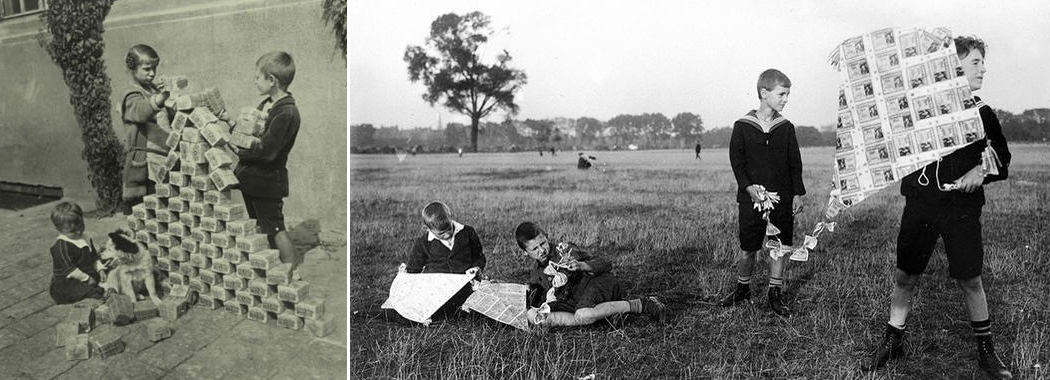
\includegraphics{assets/images/children-playing-with-money.png}
  \caption{Hyperinflation in the Weimar Republic (1921-1923)}
  \label{fig:children-playing-with-money}
\end{figure}

\paragraph{} Penge falder også i værdi med såkaldt \enquote{mild} inflation. Det sker bare langsomt nok til, at de fleste mennesker ikke lægger mærke til, at deres købekraft mindskes. Og når først seddelpresserne kører, kan hvad der før var mild inflation, med et tryk på en knap, blive til højere inflation. Som Friedrich Hayek påpegede i et af sine essays, fører mild inflation som regel til decideret inflation.\begin{quotation}\begin{samepage} \enquote{`En mild, stabil inflation hjælper ikke - den kan kun føre til decideret inflation.} \begin{flushright} -- Friedrich Hayek\footnote{Friedrich Hayek, \textit{1980s Unemployment and the Unions} \cite{hayek-inflation}}
\end{flushright}\end{samepage}\end{quotation}

Inflation er især lusket, fordi den favoriserer dem, der er tættere på seddelpresserne. Det tager tid for de nyskabte penge at cirkulere og priserne at tilpasse sig, så hvis du er i stand til at få fat i flere penge, før alle penge devalueres, er du foran inflationskurven. Det er også derfor, at inflation kan ses som en skjult skat, fordi staten i sidste ende tjener på det, mens alle andre ender med at betale prisen.\begin{quotation}\begin{samepage} \enquote{Jeg tror ikke, det er en overdrivelse at sige, at historie i høj grad omhandler inflation, og som regel inflation, der er skabt af stater for deres egen vindings skyld.} \begin{flushright} -- Friedrich Hayek\footnote{Friedrich Hayek, \textit{Good Money} \cite{hayek-good-money}}
\end{flushright}\end{samepage}\end{quotation}

\newpage

Indtil videre er alle statskontrollerede valutaer med tiden blevet erstattet eller kollapset fuldstændig. Uanset hvor lille inflationsraten er, er \enquote{stabil} vækst bare en anden måde at sige eksponentiel vækst. I naturen, som i økonomien, vil alle systemer, der vokser eksponentielt, til sidst flade ud eller lide af et katastrofalt sammenbrud.\paragraph{} \enquote{Det kan ikke ske i mit land} tænker du sikkert. Det tænker du ikke, hvis du er fra Venezuela, som i øjeblikket lider af hyperinflation. Med en inflationsrate på over 1 million procent er penge stort set værdiløse. \cite{wiki:venezuela}

\paragraph{} Det sker måske ikke inden for de næste par år, eller med den valuta, der bruges i dit land. Men et blik på listen over historiske valutaer\footnote{Se \textit{List of historical currencies} på den engelske udgave af Wikipedia. \cite{wiki:historical-currencies}} viser, at det uundgåeligt vil ske over en tilstrækkelig lang periode. Jeg husker og brugte mange af de nævnte: den østrigske schilling, den tyske mark, den italienske lire, den franske franc, det irske pund, den kroatiske dinar osv. Min bedstemor brugte endda den østrig-ungarske krone. Som tiden går, bliver de valutaer, der i øjeblikket bruges\footnote{Se \textit{List of currencies} på den engelske udgave af Wikipedia \cite{wiki:list-of-currencies}} vil langsomt, men sikkert bevæge sig mod deres respektive kirkegårde. De vil opleve hyperinflation eller blive erstattet. De vil snart være historiske valutaer. Vi vil gøre dem forældede.\begin{quotation}\begin{samepage} \enquote{Historien har vist, at staterne uundgåeligt vil falde for fristelsen til at øge pengemængden.} \begin{flushright} -- Saifedean Ammous\footnote{Saifedean Ammous, \textit{Bitcoinstandarden} \cite{bitcoin-standard}}
\end{flushright}\end{samepage}\end{quotation}

\newpage

Hvorfor er Bitcoin anderledes? I modsætning til statslige valutaer, er monetære varer ikke reguleret af stater, men af fysikkens love\footnote{Gigi, \textit{Bitcoin's Energy Consumption - A shift in perspective} \cite{gigi:energy}}, have en tendens til at overleve og endda bevare deres respektive værdi over tid. Det bedste eksempel på dette indtil videre er guld, som med det passende navn \textit{Guld-til-anstændigt-jakkesæt-forhold}\footnote{Historien viser, at prisen på en ounce (31,1 gram) guld svarer til prisen på et anstændigt jakkesæt, ifølge Sionnas investeringsforvaltere \cite{web:gold-to-decent-suite-ratio}} bevarer den sin værdi over hundreder og endda tusinde år. Den er muligvis ikke perfekt \enquote{stabilt} - et tvivlsomt koncept i første omgang - men den værdi, det har, vil i det mindste være i samme størrelsesorden.

Hvis en monetær vare eller valuta er god til at fastholde sin værdi over tid og rum, anses den for at være \textit{hård}. Hvis den ikke formår at opretholde sin værdi, på grund af nem forringelse eller inflation, betragtes den som en \textit{blød} valuta. Begrebet hårdhed er essentielt for at forstå Bitcoin og fortjener en grundigere undersøgelse. Vi vil tage emnet op igen i den sidste økonomilektion: stabile penge.\paragraph{} Efterhånden som flere og flere lande rammes af hyperinflation, vil flere og flere mennesker blive nødt til at forholde sig til virkeligheden med hårde og bløde penge. Hvis vi er heldige, vil nogle centralbankchefer måske endda blive tvunget til at revurdere deres pengepolitiske strategier. Uanset hvad der måtte ske, vil den indsigt, jeg har fået takket være Bitcoin, sandsynligvis være uvurderlig, uanset udfaldet.\paragraph{Bitcoin har lært mig om den skjulte skat ved inflation samt katastrofen forbundet med hyperinflation.}% ---
%
% #### Down the Rabbit Hole
%
% - [Economics in One Lesson][Henry Hazlitt] by Henry Hazlitt
% - [1980's Unemployment and the Unions][unions] by Friedrich Hayek
% - [Good Money, Part II][good-money]: Volume Six of the Collected Works of F.A. Hayek
% - [The Bitcoin Standard] by Saifedean Ammous
% - [Hyperinflation][hyperinflates], [economic crisis in Venezuela][wiki-venezuela], [list of historical currencies], [list of currencies][currently in use] on Wikipedia
%
% [unions]: https://books.google.com/books/about/1980s_unemployment_and_the_unions.html?id=xM9CAQAAIAAJ
% [good-money]: https://books.google.com/books?id=l_A1vVIaYBYC
%
% [Henry Hazlitt]: https://mises.org/library/economics-one-lesson
% [hyperinflates]: https://en.wikipedia.org/wiki/Hyperinflation
% [inflation cannot help]: https://books.google.com/books?id=zZu3AAAAIAAJ&dq=%22only+while+it+accelerates%22&focus=searchwithinvolume&q=%22steady+inflation+cannot+help%22
% [history of inflation]: https://books.google.com/books?id=l_A1vVIaYBYC&pg=PA142&dq=%22history+is+largely+a+history+of+inflation%22&hl=en&sa=X&ved=0ahUKEwi90NDLrdnfAhUprVkKHUx1CmIQ6AEIKjAA#v=onepage&q=%22history%20is%20largely%20a%20history%20of%20inflation%22&f=false
% [wiki-venezuela]: https://en.wikipedia.org/wiki/Crisis_in_Venezuela#Economic_crisis
% [by the laws of physics]: https://link.medium.com/9fzq2L0J3S
% [\textit{Gold-to-Decent-Suit Ratio}]: https://www.businesswire.com/news/home/20110819005774/en/History-Shows-Price-Ounce-Gold-Equals-Price
% [The Bitcoin Standard]: https://thesaifhouse.wordpress.com/book/
%
% <!-- Wikipedia -->
% [alice]: https://en.wikipedia.org/wiki/Alice%27s_Adventures_in_Wonderland
% [carroll]: https://en.wikipedia.org/wiki/Lewis_Carroll

\chapter{Værdi}
\label{les:10}

\begin{chapquote}{Lewis Carroll, \textit{Alice i Eventyrland}}
\enquote{Det var den hvide kanin, der traskede langsomt tilbage igen og så sig ængsteligt omkring, som om den havde mistet noget\ldots}
\end{chapquote}

Værdi er på en måde paradoksal, og der er flere teorier\footnote{Se \textit{Theory of value (economics)} på den engelske udgave af Wikipedia \cite{wiki:theory-of-value}} som forsøger at forklare, hvorfor vi værdsætter visse ting frem for andre ting. Dette paradoks har mennesker været opmærksomme på i tusinder af år. Som Platon skrev i sin dialog med Euthydemus, værdsætter vi nogle ting, fordi de er sjældne, og ikke blot på grund af deres nødvendighed for vores overlevelse.\begin{quotation}\begin{samepage} \enquote{Og hvis du er fornuftig, vil du også give dette råd til dine elever - at de aldrig skal konversere med nogen bortset fra dig og hinanden. For det er det sjældne, Euthydemus, der er dyrebart, mens vand er det billigste, skønt det er det bedste, som Pindar sagde.} \begin{flushright} -- Platon\footnote{Platon, \textit{Euthydemus} \cite{euthydemus}}
\end{flushright}\end{samepage}\end{quotation}

Dette paradoks af værdi\footnote{Se \textit{Paradox of value} på den engelske udgave af Wikipedia \cite{wiki:paradox-of-value}} viser noget interessant om os mennesker: Det virker, som om vi værdsætter ting på et subjektivt\footnote{Se \textit{Subjective theory of value} på den engelske udgave af Wikipedia \cite{wiki:subjective-theory-of-value}} grundlag, men gør det med visse ikke-tilfældige kriterier. Noget kan være \textit{dyrebart} for os af forskellige årsager, men ting vi værdsætter, deler visse karakteristika. Hvis vi let kan kopiere noget, eller hvis det er i naturligt overflod, værdsætter vi det ikke.

Det ser ud til, at vi værdsætter noget, fordi det er knapt (guld, diamanter, tid), svært eller arbejdskrævende at producere, uerstatteligt (et gammelt fotografi af en, vi elsker), er nyttigt på en måde, hvor det gør os i stand til at gøre ting, vi ellers ikke kunne, eller en kombination af disse, såsom store kunstværker.

Bitcoin er alt det ovenstående: Den er ekstrem knap (21 millioner), stadig sværere at producere (blokbelønning halveres), kan ikke erstattes (en tabt privat nøgle er tabt for evigt) og gør det muligt for os at udføre nogle ret nyttige ting. Det er uden tvivl det bedste værktøj til værdioverførsel på tværs af grænser, modstandsdygtigt over for censur og konfiskation i processen. Den er også et selvstændig værdilager, der giver enkeltpersoner mulighed for at opbevare deres formue uafhængigt af banker og stater. Bare for at nævne et par ting.\paragraph{Bitcoin har lært mig, at værdi er subjektiv, men ikke vilkårlig.}% ---
%
% #### Down the Rabbit Hole
%
% - [Euthydemus] by Plato
% - [Theory of Value][multiple theories], [Paradox of Value][paradox of value], [Subjective Theory of Value][subjective] on Wikipedia
%
% [Euthydemus]: http://www.perseus.tufts.edu/hopper/text?doc=Perseus:text:1999.01.0178:text=Euthyd.
% [Plato]: http://www.perseus.tufts.edu/hopper/text?doc=plat.+euthyd.+304b
%
% <!-- Wikipedia -->
% [multiple theories]: https://en.wikipedia.org/wiki/Theory_of_value_%28economics%29
% [paradox of value]: https://en.wikipedia.org/wiki/Paradox_of_value
% [subjective]: https://en.wikipedia.org/wiki/Subjective_theory_of_value
% [alice]: https://en.wikipedia.org/wiki/Alice%27s_Adventures_in_Wonderland
% [carroll]: https://en.wikipedia.org/wiki/Lewis_Carroll

\chapter{Penge}
\label{les:11}

\begin{chapquote}{Den vise}
\enquote{I min ungdom, \ldots \\ Holdt jeg alle mine lemmer meget smidige, \\ Ved brug af denne salve, \\ Fem shillinger pr. æske -- \\ Tillad mig at sælge dig et par stykker.}
\end{chapquote}

Hvad er penge? Vi bruger dem hver dag, men alligevel er dette spørgsmål overraskende svært at besvare. Vi er afhængige af dem i stort og småt, og hvis vi har for få, bliver vores liv meget vanskeligt. Alligevel tænker vi sjældent over den ting, der angiveligt får verden til at dreje rundt. Bitcoin har tvunget mig til at besvare det samme spørgsmål igen og igen: Hvad pokker er penge overhovedet?

I vores \enquote{moderne} verden vil de fleste nok tænke på papirstykker, når de taler om penge, selvom de fleste af vores penge bare er et tal på en bankkonto. Vi bruger allerede nuller og ettaller som vores penge, så hvordan er Bitcoin anderledes? Bitcoin er anderledes, fordi det i sin kerne er en meget anderledes \textit{type} penge end de penge, vi bruger i øjeblikket. For at forstå dette bliver vi nødt til at se nærmere på, hvad penge er, hvordan de blev til, og hvorfor guld og sølv blev brugt i det meste af handelshistorien.\paragraph{} Muslingeskaller, guld, sølv, papir, bitcoin. I sidste ende \textbf{er penge det, som folk accepterer som betalingsmiddel}, uanset dets form eller mangel på samme.

Penge er en genial opfindelse. En verden uden penge er vanvittigt kompliceret: Hvor mange fisk koster et par nye sko? Hvor mange køer koster et nyt hus? Hvad nu, hvis jeg ikke har brug for noget lige nu, men er nødt til at skille mig af med mine snart rådne æbler? Man behøver ikke meget fantasi for at indse, at en byttehandel er vanvittigt ineffektiv.

Det fantastiske ved penge er, at de kan veksles til \textit{alt muligt andet} - det er noget af en opfindelse! Som Nick Szabo\footnote{\url{http://unenumerated.blogspot.com/}} sammenfatter på glimrende vis i \textit{Shelling Out: The Origins of Money} \cite{shelling-out}, har vi mennesker brugt alle mulige ting som penge: perler lavet af sjældne materialer som elfenben, skaller eller særlige knogler, forskellige slags smykker og senere sjældne metaller som sølv og guld.\begin{quotation}\begin{samepage} \enquote{I den forstand minder den (Bitcoin) mere om et ædelmetal. I stedet for at udbuddet ændrer sig for at holde værdien den samme, er udbuddet forudbestemt, og værdien ændrer sig.} \begin{flushright} -- Satoshi Nakamoto\footnote{Satoshi Nakamoto, i et svar til Sepp Hasslberger \cite{satoshi-precious-metal}}
\end{flushright}\end{samepage}\end{quotation}

Som de dovne væsener vi er, tænker vi ikke så meget over ting, der bare fungerer. For de fleste af os fungerer penge helt fint. Ligesom med vores biler eller computere er de fleste af os kun tvunget til at tænke over disse tings indre funktion, hvis de bryder sammen. Folk, der har set deres livsopsparing forsvinde på grund af hyperinflation, kender værdien af stærke penge, ligesom folk, der har set deres venner og familie forsvinde på grund af grusomhederne i Nazityskland eller Sovjetunionen forstår værdien af privatliv.

Det særlige ved penge er, at de er altomfattende. Penge er halvdelen af enhver transaktion, hvilket giver dem, der har ansvaret for at skabe penge, en enorm magt.\begin{quotation}\begin{samepage} \enquote{I betragtning af at penge udgør halvdelen af alle kommercielle transaktioner, og at hele civilisationer bogstaveligt talt opstår og falder på baggrund af kvaliteten af deres penge, taler vi om en fantastisk magt, som foregår i det skjulte. Det er magten til at skabe illusioner, der fremstår virkelige, så længe de varer. Det er selve kernen af centralbankernes magt.} \begin{flushright} -- Ron Paul\footnote{Ron Paul, \textit{End the Fed} (Afskaf den amerikanske centralbank) \cite{end-the-fed}}
\end{flushright}\end{samepage}\end{quotation}

Bitcoin fjerner denne magt på fredelig vis, da den fjerner skabelsen af penge uden brug af magt.

Pengene gennemgik flere iterationer. De fleste iterationer var gode. De forbedrede vores penge på den ene eller anden måde. Men for ganske nylig blev vores penges indre funktioner korrupte. I dag er næsten alle vores penge simpelthen skabt \textit{ud af den blå luft} af magthaverne. For at forstå, hvordan det kunne ske, var jeg nødt til at lære om pengenes historie og efterfølgende undergang.

Om det vil kræve en række katastrofer, eller blot en enorm uddannelsesindsats for at rette op på denne korruption, er endnu uvist. Jeg beder til guderne for stabile penge om, at det bliver det sidste.\paragraph{Bitcoin har lært mig, hvad penge er.}% ---
%
% #### Down the Rabbit Hole
%
% - [End the Fed][Ron Paul] by Ron Paul
% - [Money, blockchains, and social scalability][social-scalability] by Nick Szabo
%
% [social-scalability]: https://unenumerated.blogspot.co.at/2017/02/money-blockchains-and-social-scalability.html
%

\chapter{Pengenes historie og undergang}
\label{les:12}

\begin{chapquote}{Lewis Carroll, \textit{Alice i Eventyrland}} \enquote{De ville ikke huske de enkle regler, som deres venner havde givet dem, såsom at hvis man går ind i ilden, vil den brænde en, og at hvis man skærer sig meget dybt i fingeren med en kniv, bløder det som regel, og hun havde aldrig glemt, at hvis man drikker af en flaske, hvor der står \enquote{gift}, er det næsten sikkert, at det giver problemer før eller siden.} \end{chapquote}

Mange mennesker tror, at penge er understøttet af guld, som er låst væk i store bankbokse, beskyttet af tykke mure. Det stoppede med at være sandt for mange årtier siden. Jeg er ikke sikker på, hvad jeg tænkte dengang, for jeg var i meget større problemer og havde stort set ingen forståelse af guld, papirpenge, eller hvorfor de overhovedet skulle være understøttet af noget.

En del af processen med at lære om Bitcoin er at forstå fiat-penge: hvad de betyder, hvordan de opstod, og hvorfor de måske ikke er den bedste id\'e, vi nogensinde har haft. Så hvad er fiat-penge egentlig? Og hvordan endte vi med at bruge dem?

Hvis noget er pålagt ved \textit{fiat}, betyder det blot, at det er pålagt gennem en formel godkendelse eller et forslag. Således er fiat-penge penge, blot fordi \textit{nogen} siger, at de er penge. Da alle stater bruger fiat-penge i dag, gælder det også \textit{din} stat. Desværre er du ikke \textit{fri} til at være uenig i dette værdiforslag. Du vil hurtigt føle, at dette forslag er alt andet end ikke-voldeligt. Hvis du nægter at bruge denne papirvaluta til at drive forretninger og betale skat, vil de eneste mennesker, du vil kunne diskutere økonomi med, være dine cellekammerater.

Værdien af fiat-penge stammer ikke fra deres indbyggede egenskaber. Hvor gode en bestemt type fiat-penge er, hænger kun sammen med den politiske og skattemæssige ustabilitet hos dem, der drømmer dem frem. Deres værdi pålægges ved dekret, vilkårligt.\begin{figure}
  \centering
  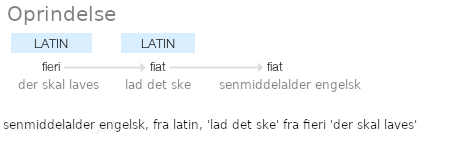
\includegraphics[width=8cm]{assets/images/fiat-definition.png}
  \caption{fiat — `Lad det ske'}
  \label{fig:fiat-definition}
\end{figure}

\paragraph{} Indtil for nylig brugte man to typer af penge: \textbf{varepenge}, lavet af værdifulde \textit{ting}, og \textbf{repræsentative penge}, som blot \textit{repræsenterer} den værdifulde ting, for det meste på skrift.\paragraph{} Vi har allerede været inde på varepenge ovenfor. Folk brugte særlige knogler, muslingeskaller og ædelmetaller som penge. Senere blev det især mønter lavet af ædelmetaller som guld og sølv, der blev brugt som penge. Den ældste mønt, der indtil videre er blevet fundet, er fremstillet af en naturlig blanding af guld og sølv, og blev produceret for mere end 2700 år siden.\footnote{Ifølge den græske historiker Herodot, der skrev i det femte århundrede f.Kr., var lydierne det første folk, der brugte guld- og sølvmønter. \cite{coinage-origins}} Hvis noget er nyt ved Bitcoin, er det ikke konceptet \textit{coin} (mønt).\newpage

\begin{figure}
  \centering
  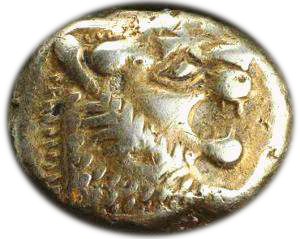
\includegraphics[width=5cm]{assets/images/lydian-coin-stater.png}
  \caption{Lydisk mønt. Billedet er licenseret under Creative Commons Attribution Share-Alike 4.0 af Classical Numismatic Group, Inc.}
  \label{fig:lydian-coin-stater}
\end{figure}

Det viser sig, at hamstring af mønter, eller \textit{hodling}, for at bruge nutidens sprog, er næsten lige så gammelt som mønter. Den tidligste mønthamstrer var en person, der lagde næsten hundrede af disse mønter i en krukke og begravede den i fundamentet til et tempel, som først blev fundet 2.500 år senere. Det er en ret god offline opbevaring, hvis du spørger mig.

Én af ulemperne ved at bruge ædelmetalmønter er, at de kan blive klippet, hvilket effektivt forringer møntens værdi. Nye mønter kan blive præget af de afklippede mønter, hvilket øger pengemængden over tid og devaluerer hver enkelt mønt i processen. Folk barberede bogstaveligt talt så meget af deres sølvdollars, som de kunne slippe afsted med.

Da stater kun er glade for inflation, hvis det er dem, der skaber den, blev der gjort en indsats for at stoppe denne guerilla-devaluering. På klassisk politi-og-røver-man\'er blev møntklipperne stadig mere kreative med deres teknikker, hvilket tvang \enquote{mønt-mestrene} til at blive endnu mere kreative med deres modforanstaltninger. Isaac Newton, den verdensberømte fysiker, der er kendt for \textit{Principia Mathematica}, var en af disse mestre. Han tilskrives æren for at have tilføjet de små striber på siden af mønterne, som stadig kan ses den dag i dag. Tiden med nem møntbarbering var forbi.\begin{figure}
  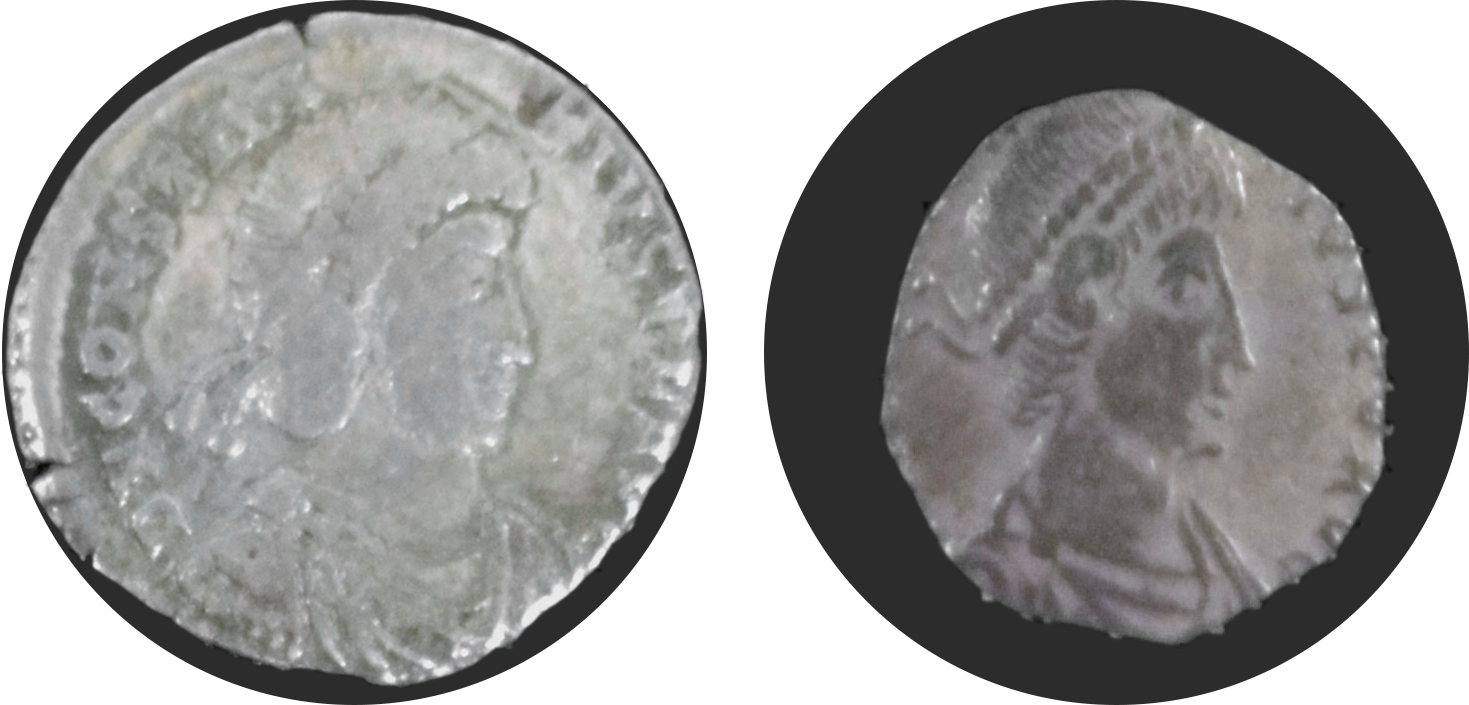
\includegraphics{assets/images/clipped-coins.png}
  \caption{Sølvmønter med varierende grad af afklipning.}
  \label{fig:clipped-coins}
\end{figure}

Selv med disse metoder til devaluering af mønter\footnote{Udover at klippe mønterne, var svedning (at ryste mønterne i en pose og opsamle det støv, der blev slidt af) og tilstopning (at slå et hul i midten og hamre mønten flad for at lukke hullet) de mest fremtrædende metoder til devaluering af mønter. \cite{wiki:coin-debasement}} holdt i skak, har de stadig andre problemer. De er klodsede og ikke særlig praktiske at transportere, især når der skal ske store værdioverførsler. Det er ikke særlig praktisk at dukke op med en stor pose sølvdollars, hver gang du vil købe en Mercedes.

Nu vi taler om tyske ting: Hvordan den amerikanske \textit{dollar} fik sit navn, er en anden interessant historie. Ordet \enquote{dollar} er afledt af det tyske ord \textit{Thaler}, en forkortelse for \textit{Joachimsthaler}~\cite{wiki:thaler}. En Joachimsthaler var en mønt, der blev præget i byen \textit{Sankt Joachimsthal}. Thaler er simpelthen en forkortelse for nogen (eller noget), der kommer fra dalen, og fordi Joachimsthal var \textit{dalen} for sølvmøntproduktion, omtalte folk simpelthen disse sølvmønter som \textit{Thaler.} Thaler (tysk) blev til daalders (hollandsk) og til sidst dollars (engelsk).\begin{figure}
  \centering
  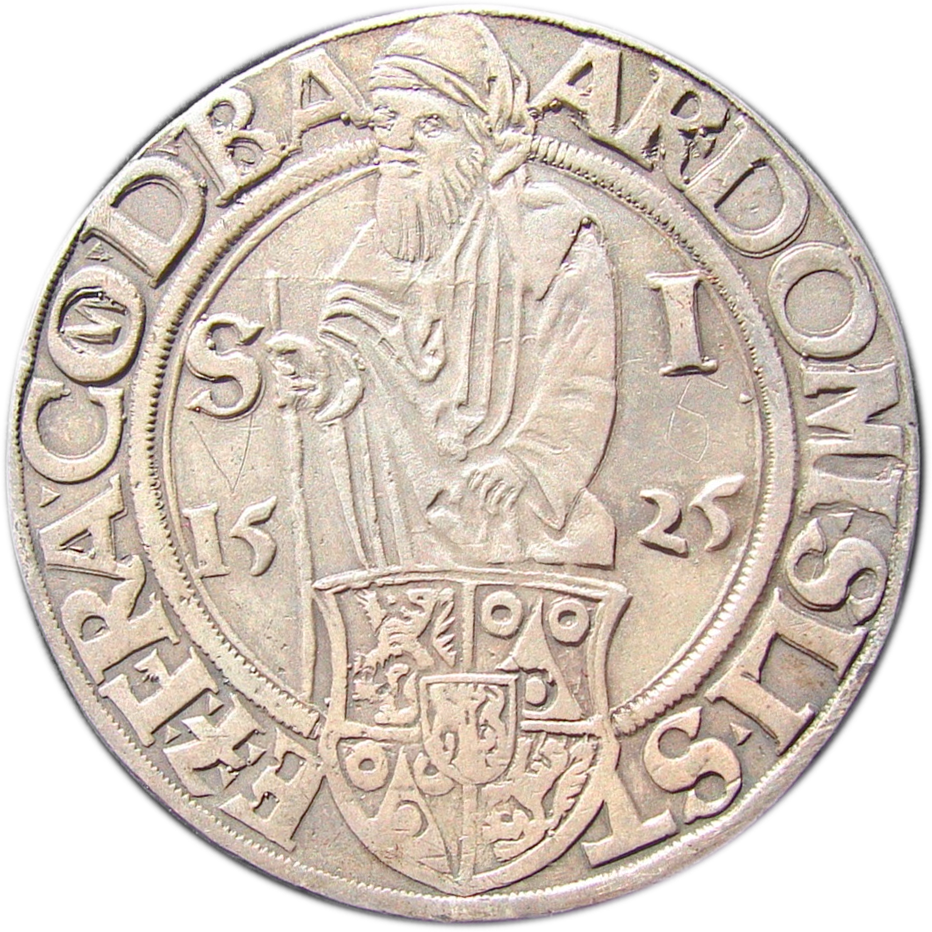
\includegraphics[width=5cm]{assets/images/joachimsthaler.png}
  \caption{Den oprindelige \enquote{dollar}. Sankt Joachim er afbilledet med sin kappe og troldmandshat. Billedet er cc-by-sa af Wikipedia-bruger Berlin-George}
  \label{fig:joachimsthaler}
\end{figure}

Indførelsen af repræsentative penge indvarslede de stærke penges undergang. Guldcertifikater blev introduceret i 1863, og omkring femten år senere blev sølvdollaren også langsomt, men sikkert erstattet af gældsbeviser: sølvcertifikatet. \cite{wiki:silver-certificate}

Det tog omkring 50 år fra introduktionen af de første sølv-certifikater, til disse stykker papir blev forvandlet til noget, som vi i dag ville genkende som en amerikansk dollar.\begin{figure}
  \centering
  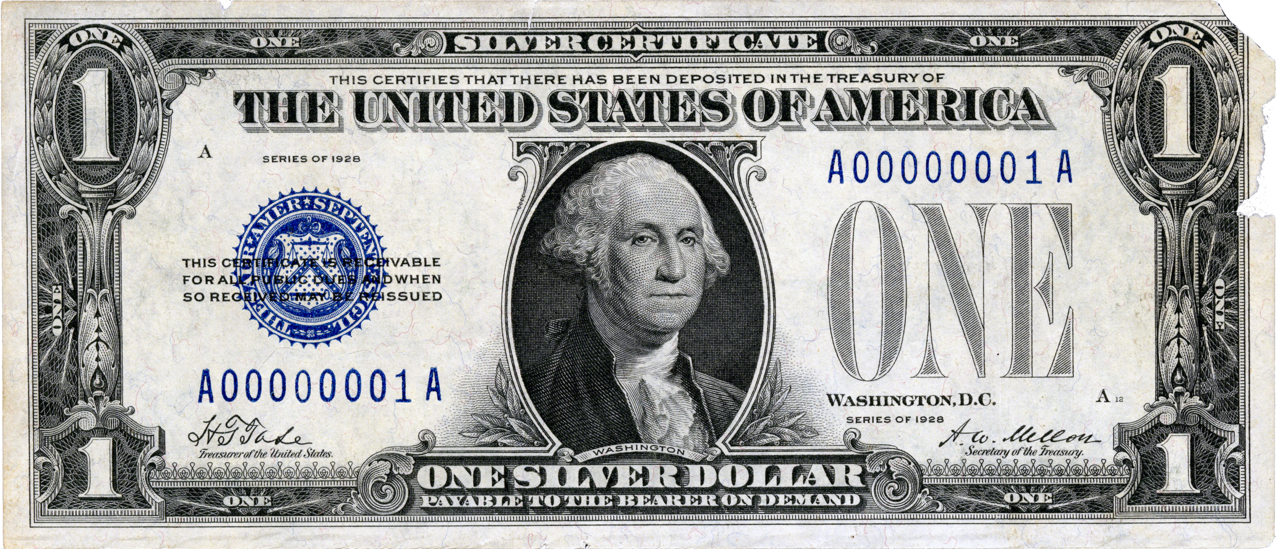
\includegraphics{assets/images/us-silver-dollar-note-smaller.png}
  \caption{En amerikansk sølvdollar fra 1928. \enquote{Betales til ihændehaveren på forespørgsel.} Billede cc-by-sa af National Numismatic Collection ved the Smithsonian Institution}
  \label{fig:us-silver-dollar-note-smaller}
\end{figure}

Bemærk, at den amerikanske sølvdollar fra 1928 i figur~\ref{fig:us-silver-dollar-note-smaller} stadig går under navnet \textit{sølvcertifikat}, hvilket indikerer, at dette faktisk blot er et dokument, der angiver, at indehaveren af dette stykke papir har krav på et stykke sølv. Det er interessant at se, hvordan teksten, der indikerer dette, er blevet mindre fremtrædende over tid. Sporet af \enquote{certifikat} forsvandt helt efter et stykke tid og blev erstattet af den beroligende erklæring om, at dette er Federal Reserves sedler.

Som nævnt ovenfor, skete det samme med guld. Det meste af verden havde en bimetallisk standard~\cite{wiki:bimetallism}, hvilket betyder, at mønter primært var lavet af guld og sølv. At have certifikater for guld, som kunne indløses til guldmønter, var sandsynligvis en teknologisk forbedring. Papir er mere praktisk, lettere, og da det kan opdeles vilkårligt blot ved at printe et mindre tal, er det lettere at opdele i mindre enheder.

For at minde indehaverne (brugerne) om, at disse certifikater var repræsentative for ægte guld og sølv, blev de farvet i overensstemmelse hermed, og det fremgik tydeligt af selve certifikatet. Du kan læse skriften flydende fra top til bund.\begin{quotation}\begin{samepage} \enquote{Dette bekræfter, at der er deponeret et hundrede dollars i guldmønt i USA's skatkammer, som kan udbetales til ihændehaveren på forespørgsel.} \end{samepage}\end{quotation}

\begin{figure}
  \centering
  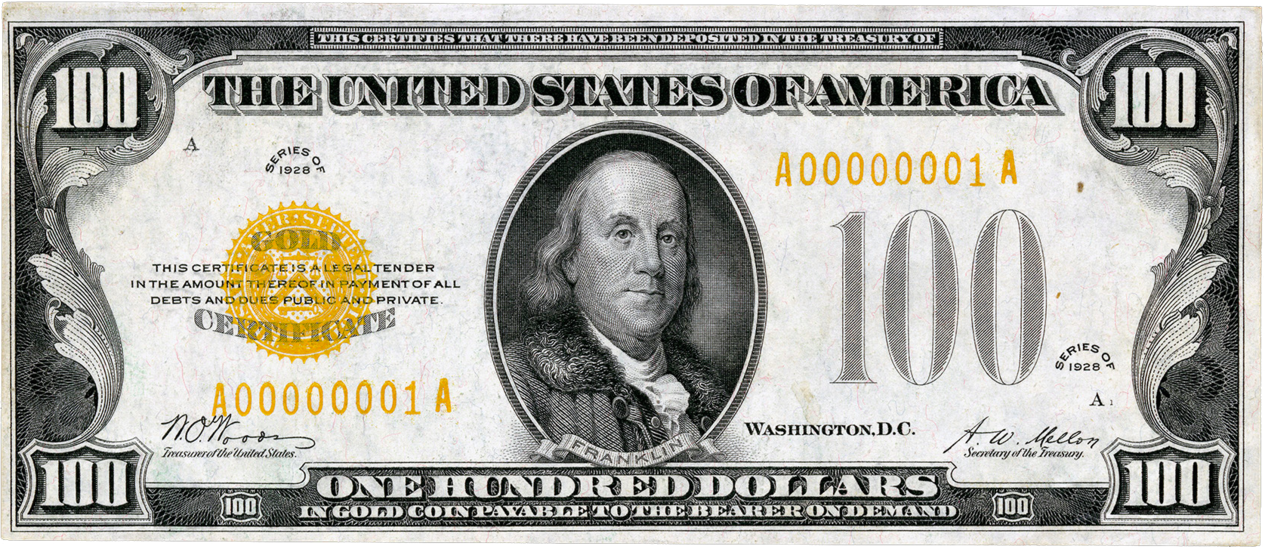
\includegraphics{assets/images/us-gold-cert-100-smaller.png}
  \caption{Dette er et amerikansk 100 dollars guldcertifikat fra 1928. Billedet er cc-by-sa fra National Numismatic Collection, National Museum of American History.}
  \label{fig:us-gold-cert-100-smaller}
\end{figure}

I 1963 blev ordene \enquote{PAYABLE TO THE BEARER ON DEMAND} (betales til ihændehaveren på forespørgsel) fjernet fra alle nyudstedte sedler. Fem år senere ophørte indløsningen af papirsedler til guld og sølv.

De ord, som hentyder til oprindelsen og id\'een bag papirpenge, blev fjernet. Den gyldne farve forsvandt. Det eneste, der blev tilbage, var papiret og dermed statens mulighed for at trykke så mange sedler, som den ønsker.

Afskaffelsen af guldstandarden i 1971 fuldendte dette århundrede-lange trick. Penge blev forvandlet til den illusion, vi alle deler den dag i dag: fiat-penge. De har værdi, fordi dem, der har kommandoen over en hær og driver fængsler, siger, at de har værdi. Som man tydeligt kan læse på enhver dollarseddel, der er i omløb i dag: \enquote{DENNE SEDDEL ER LOVLIGT BETALINGSMIDDEL}. Med andre ord: Den har værdi, fordi sedlen siger det.\begin{figure}
  \centering
  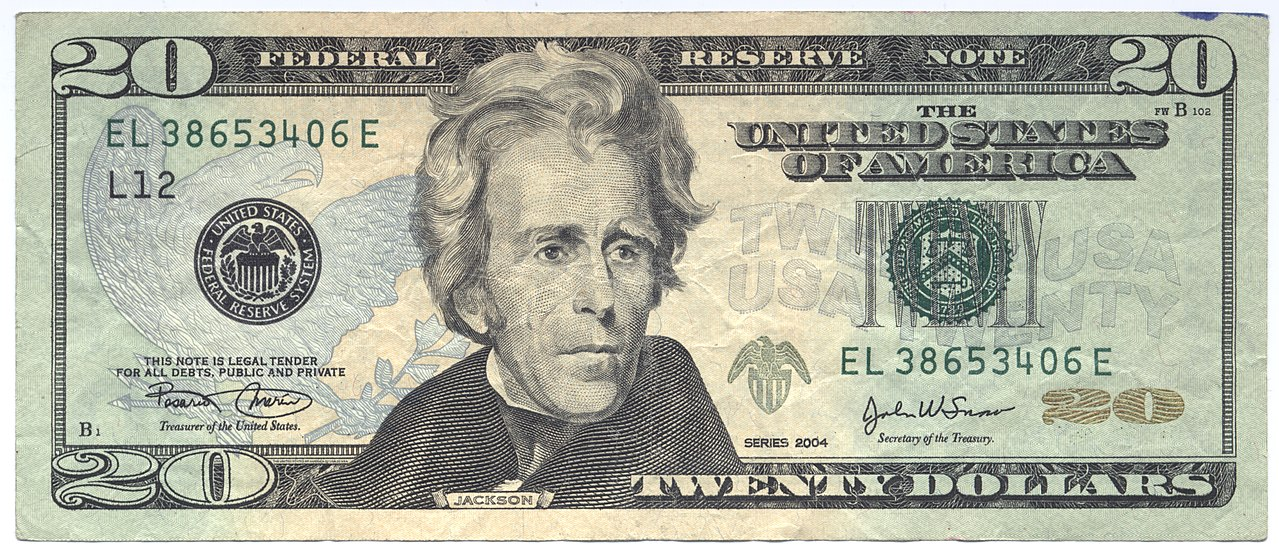
\includegraphics{assets/images/us-dollar-2004.jpg}
  \caption{En 20-dollarseddel fra 2004-serien, der bruges i dag. `DENNE SEDDEL ER LOVLIGT BETALINGSMIDDEL'}
  \label{fig:us-dollar-2004}
\end{figure}

I øvrigt er der en anden interessant lektion i nutidens pengesedler, skjult i det åbne. På den anden linje står der, at dette er et lovligt betalingsmiddel \enquote{FOR AL GÆLD, OFFENTLIG OG PRIVAT}. Hvad der måske er indlysende for økonomer, var overraskende for mig: Alle penge er gæld. Jeg har stadig ondt i hovedet på grund af det, og jeg vil overlade udforskningen af forholdet mellem penge og gæld som en øvelse til læseren.\paragraph{} Som vi har set, blev guld og sølv brugt som penge i årtusinder. Med tiden blev mønter lavet af guld og sølv erstattet af papir. Papir blev langsomt accepteret som betaling. Denne accept skabte en illusion - illusionen om, at papiret i sig selv har værdi. Det sidste skridt var helt at afbryde forbindelsen mellem repræsentationen og det faktiske: at afskaffe guldstandarden og overbevise alle om, at papiret i sig selv er værdifuldt.\paragraph{Bitcoin har lært mig om pengenes historie og det største trick i økonomiens historie: fiat-valuta.}% ---
%
% #### Down the Rabbit Hole
%
% - [Shelling Out: The Origins of Money] by Nick Szabo
% - [Methods of Coin Debasement][coin debasement], [Thaler], [U.S. Silver Certificate][silver certificates], [Bimetallism][bimetallic standard] on Wikipedia
%
% [oldest coin]: https://www.britishmuseum.org/explore/themes/money/the_origins_of_coinage.aspx
% [coin debasement]: https://en.wikipedia.org/wiki/Methods_of_coin_debasement
% [Thaler]: https://en.wikipedia.org/wiki/Thaler
% [Berlin-George]: https://en.wikipedia.org/wiki/File:Bohemia,_Joachimsthaler_1525_Electrotype_Copy._VF._Obverse..jpg
% [silver certificates]: https://en.wikipedia.org/wiki/Silver_certificate_%28United_States%29
% [bimetallic standard]: https://en.wikipedia.org/wiki/Bimetallism
% [Shelling Out: The Origins of Money]: https://nakamotoinstitute.org/shelling-out/
%
% <!-- Wikipedia -->
% [alice]: https://en.wikipedia.org/wiki/Alice%27s_Adventures_in_Wonderland
% [carroll]: https://en.wikipedia.org/wiki/Lewis_Carroll

\chapter{Vanviddet i brøkreserve-bankvæsenet}
\label{les:13}

\begin{chapquote}{Lewis Carroll, \textit{Alice i Eventyrland}} Men ak, - det var for sent at ønske! Hun blev ved med at vokse og vokse, og snart måtte hun knæle ned på gulvet. Men lidt efter var der ikke engang plads til det, og hun prøvede nu at lægge sig helt ned, med den ene albue mod døren og den anden under hovedet. Hun blev imidlertid ved med at vokse, og til sidst havde hun ingen anden udvej end at stikke den ene arm ud ad vinduet og foden op i skorstenen. Så sagde hun: \enquote{Nu kan jeg ikke gøre mere, hvad der end sker. Hvad skal der dog blive af mig?} \end{chapquote}

Værdi og penge er ikke trivielle emner, især ikke i vor tid. Processen med at skabe penge i vores banksystem er heller ikke triviel, og jeg kan ikke slippe følelsen af, at det er bevidst. Det, jeg tidligere kun er stødt på i akademiske og juridiske tekster, ser også ud til at være almindelig praksis i finansverdenen: Intet forklares i enkle vendinger, ikke fordi det virkelig er komplekst, men fordi sandheden er skjult bag lag på lag af fagsprog og \textit{tilsyneladende} kompleksitet. \enquote{Ekspansiv pengepolitik, kvantitativ lempelse, finanspolitisk stimulering af økonomien.} Publikum nikker samtykkende, hypnotiseret af de fancy ord.

Brøkreservebankvæsen og kvantitativ lempelse er fancy ord, der tilslører virkeligheden ved at maskere den med kompleksitet og gøre den svær at forstå. Hvis du forklarer dem for en femårig, vil det vanvittige i dem begge hurtigt fremstå klart.

Godfrey Bloom, der talte til Europa-Parlamentet under en fælles debat, sagde det meget bedre, end jeg nogensinde kunne:\begin{quotation}\begin{samepage} \enquote{[...] Du forstår ikke rigtig, hvad en bank er. Alle banker er fallit. Bank Santander, Deutsche Bank, Royal Bank of Scotland - de er alle fallit! Og hvorfor er de fallit? Det er ikke Guds værk. Det er ikke en slags tsunami. De er fallit, fordi vi har et system, der hedder brøkreservebankvæsen, hvilket betyder, at bankerne kan låne penge ud, som de faktisk ikke har! Det er en kriminel skandale, og den har stået på alt for længe. \href{...}{} Vi har falskmøntneri - nogle gange kaldet kvantitativ lempelse - et andet navn for falskmøntneri. Den kunstige trykning af penge, som, hvis den var foretaget af en almindelig person, ville sende dem i fængsel i meget lang tid \href{...}{} og indtil vi begynder at sende bankfolk - og jeg inkluderer centralbankfolk og politikere - i fængsel for denne skændsel, vil den fortsætte.} \begin{flushright} -- Godfrey Bloom\footnote{Fælles debat om Europas bankunion~\cite{godfrey-bloom}}
\end{flushright}\end{samepage}\end{quotation}

Lad mig gentage den vigtigste del: Banker kan udlåne penge, som de faktisk ikke har.

Takket være brøkreservebankvæsen, behøver en bank kun at beholde en lille \textit{brøkdel} af hver krone, der bliver sat ind. Det er et sted mellem $0$ og $10\%$, som regel i den lave ende, hvilket gør tingene endnu værre.

Lad os bruge et konkret eksempel til bedre at forstå denne skøre id\'e: En brøkdel af $10\%$ er tilstrækkeligt, og vi bør være i stand til at foretage alle beregningerne i vores hoved. Så hvis du indsætter 100 dollars i banken - fordi du ikke vil gemme dem under din madras - så skal de kun beholde den aftalte \textit{brøkdel} af dem. I vores eksempel ville det være \$10, fordi 10\% af \$100 er \$10. Nemt, ikke?

Så hvad gør bankerne med resten af pengene? Hvad sker der med dine 90 dollars? De gør, hvad banker gør, de låner dem ud til andre mennesker. Resultatet er en pengemultiplikatoreffekt, som øger pengemængden i økonomien enormt (figur~\ref{fig:money-multiplier}). Dit oprindelige indskud på \$100 vil snart blive til \$190. Ved at udlåne 90\% af de nyoprettede \$90, vil der snart være \$271 i økonomien. Og \$343,90 derefter. Pengemængden øges rekursivt, fordi banker bogstaveligt talt låner penge, som de ikke har.~\cite{wiki:money-multiplier}. Uden et eneste abracadabra forvandler bankerne på magisk vis 100 dollars til 1.000 dollars eller mere. Det viser sig, at en ti-fords multiplikation er nemt. Det tager kun nogle få lånerunder.\begin{figure}
  \centering
  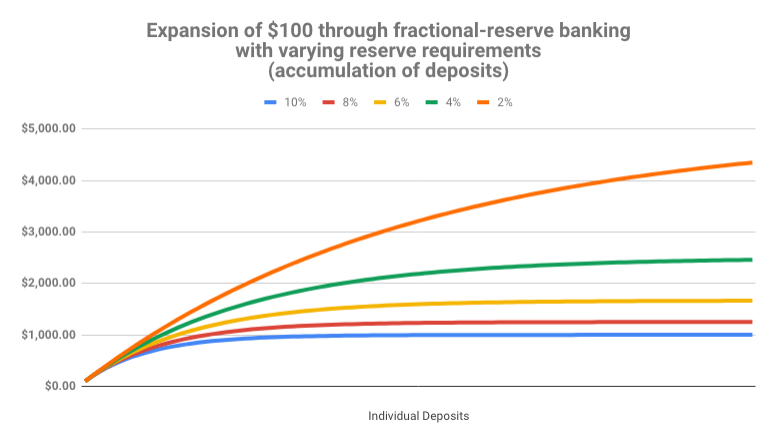
\includegraphics{assets/images/money-multiplier.png}
  \caption{Pengenes multiplikatoreffekt}
  \label{fig:money-multiplier}
\end{figure}

\paragraph{} Misforstå mig ikke: Der er ikke noget galt med at låne penge ud. Der er ikke noget galt med renter. Der er end ikke noget galt med at benytte gode, gamle, almindelige banker til at opbevare din formue et sikrere sted end i din sokkeskuffe.

Centralbanker er imidlertid en helt anden sag. De er deformiteter af finansiel regulering, delvist offentlige, delvist private. De leger Gud med noget, der påvirker os alle og som er en del af vores globale civilisation, og gør det skamløst. De er kun interesseret i den nærmeste fremtid, og tilsyneladende uden nogen form for ansvarlighed eller mulighed for revision (se figur~\ref{fig:bsg}).

\begin{figure}
  \centering
  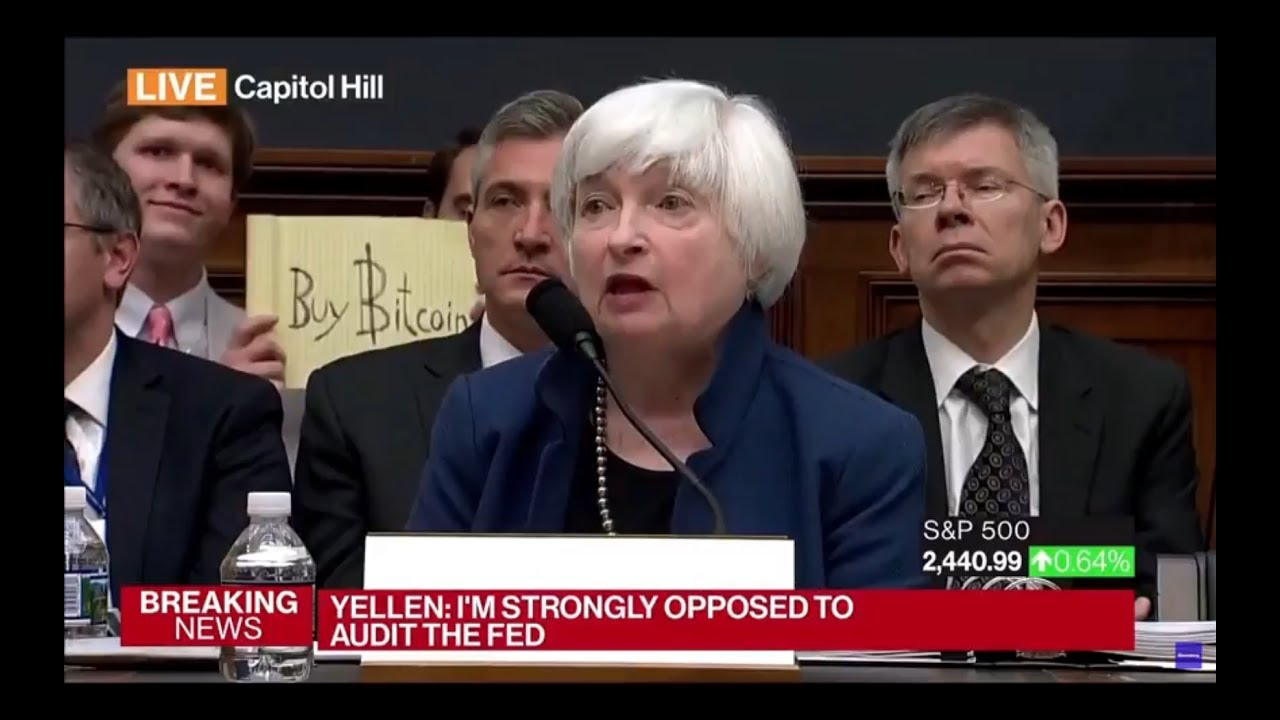
\includegraphics{assets/images/bsg.jpg}
  \caption{Yellen (direktør for den amerikanske centralbank) er en stærk modstander af en revision af den amerikanske centralbank (Federal Reserve), mens \textit{Bitcoin Sign Guy} i baggrunden stærkt argumenterer for køb af bitcoin.}
  \label{fig:bsg}
\end{figure}

Selvom Bitcoin stadig er inflationær, vil den snart ikke være det længere. Det strengt begrænsede udbud på 21 millioner bitcoins vil i sidste ende helt fjerne inflationen. Vi har nu to monetære verdener: en inflationær verden, hvor penge trykkes vilkårligt, og Bitcoins verden, hvor mængden er endelig og let at kontrollere for alle. Den ene er tvunget på os med vold, den anden er åben for alle, der ønsker at deltage. Ingen adgangsbarrierer, ingen at spørge om lov. Frivillig deltagelse. Det er det smukke ved Bitcoin.

Jeg vil argumentere for, at debatten mellem keynesianske\footnote{Teorier ifølge John Maynard Keynes og hans efterfølgere~\cite{wiki:keynesian}} og østrigske\footnote{Skolen for økonomisk tænkning baseret på metodisk individualisme er kendt som den Østrigske Økonomiske Skole~\cite{wiki:austrian}} økonomer ikke længere er rent akademisk. Satoshi formåede at bygge et system til værdioverførsel på steroider og skabte i processen de hårdeste penge, der nogensinde har eksisteret. På den ene eller anden måde vil flere og flere mennesker lære om det svindelnummer, som brøkreservebankvæsenet er. Hvis de kommer til samme konklusion som de fleste østrigere (økonomer der følger den østrigske skole) og bitcoinere, vil de måske slutte sig til det stadig voksende internet af penge. Ingen kan stoppe dem, hvis de vælger at gøre det.\paragraph{Bitcoin har lært mig, at brøkreservebankvæsen er det rene vanvid.}% ---
%
% #### Down the Rabbit Hole
%
% - [The Creature From Jekyll Island] by G. Edward Griffin
% - [Money Multiplier][money multiplier], [Keynesian Economics][Keynesian], [Austrian School][Austrian] on Wikipedia
%
% [The Creature From Jekyll Island]: https://archive.org/details/pdfy--Pori1NL6fKm2SnY
%
% [joint debate]: https://www.youtube.com/watch?v=hYzX3YZoMrs
% [money multiplier]: https://en.wikipedia.org/wiki/Money_multiplier
% [auditability]: https://i.ytimg.com/vi/ThFGs347MW8/maxresdefault.jpg
% [Keynesian]: https://en.wikipedia.org/wiki/Keynesian_economics
% [Austrian]: https://en.wikipedia.org/wiki/Austrian_School
%
% <!-- Wikipedia -->
% [alice]: https://en.wikipedia.org/wiki/Alice%27s_Adventures_in_Wonderland
% [carroll]: https://en.wikipedia.org/wiki/Lewis_Carroll

\chapter{Stabile penge}
\label{les:14}

\begin{chapquote}{Lewis Carroll, \textit{Alice i Eventyrland}} \enquote{Det første, jeg skal gøre,} sagde Alice til sig selv, mens hun vandrede rundt i skoven, \enquote{er at vokse til min rette størrelse, og det andet er at finde vej ind i den dejlige have. Jeg tror, at det vil være den bedste plan.} \end{chapquote}

Den vigtigste lektion, jeg har lært fra Bitcoin, er, at stærke penge på den lange bane er overlegne i forhold til svage penge. Stærke penge, også omtalt som \textit{stabile penge}, er enhver globalt handlet valuta, der fungerer som et pålideligt værdilager.

Selvfølgelig er Bitcoin stadig ung og volatil. Kritikere vil hævde, at den ikke lagrer værdi pålideligt. Volatilitetsargumentet misser pointen. Volatilitet er forventeligt. Det vil tage markedet et stykke tid at finde ud af, hvad den rette pris er for disse nye penge. Og som det ofte påpeges i spøg, er det baseret på en målefejl. Hvis du tænker i dollars, vil du ikke være i stand til at se, at \'en bitcoin altid vil være \'en bitcoin værd.\begin{quotation}\begin{samepage} \enquote{En fast pengemængde, eller en pengemængde, der kun ændres i overensstemmelse med objektive og beregnelige kriterier, er en nødvendig betingelse for en meningsfuld og retfærdig prisfastsættelse af penge.} \begin{flushright} -- Pater Bernard W. Dempsey, S.J.\footnote{Bernard W. Dempsey, S.J., \textit{Interest and Usury}~\cite[p.~210]{dempsey_interest_1943}}
\end{flushright}\end{samepage}\end{quotation}

\newpage

Som en hurtig tur gennem de glemte valutaers kirkegård har vist, vil penge, der kan trykkes, blive trykt. Indtil nu har ingen i historien været i stand til at modstå denne fristelse.

Bitcoin håndterer fristelsen til at trykke penge på en genial måde. Satoshi var bevidst om vores grådighed og fejlbarlighed - derfor valgte han noget mere pålideligt end menneskelig tilbageholdenhed: matematik.\begin{figure}
  \centering
  \begin{equation}
  \sum\limits_{i=0}^{32} \frac{210000 \lfloor \frac{50*10^8}{2^i} \rfloor}{10^8}
  \end{equation}
  \caption{Bitcoins forsyningsformel}
  \label{fig:supply-formula-white}
\end{figure}

Selvom denne formel er nyttig til at beskrive Bitcoins udbud, kan den faktisk ikke findes nogen steder i koden. Udstedelsen af nye bitcoin sker på en algoritmisk kontrolleret måde ved at reducere den belønning, der udbetales til minedriverne hvert fjerde år~\cite{btcwiki:supply}. Formlen ovenfor bruges til hurtigt at opsummere, hvad der sker under overfladen. Hvad der virkelig sker, kan bedst ses ved at se på ændringerne i blokbelønningen, belønningen der udbetales til den, der finder en gyldig blok, hvilket sker cirka hvert 10. minut.\begin{figure}
  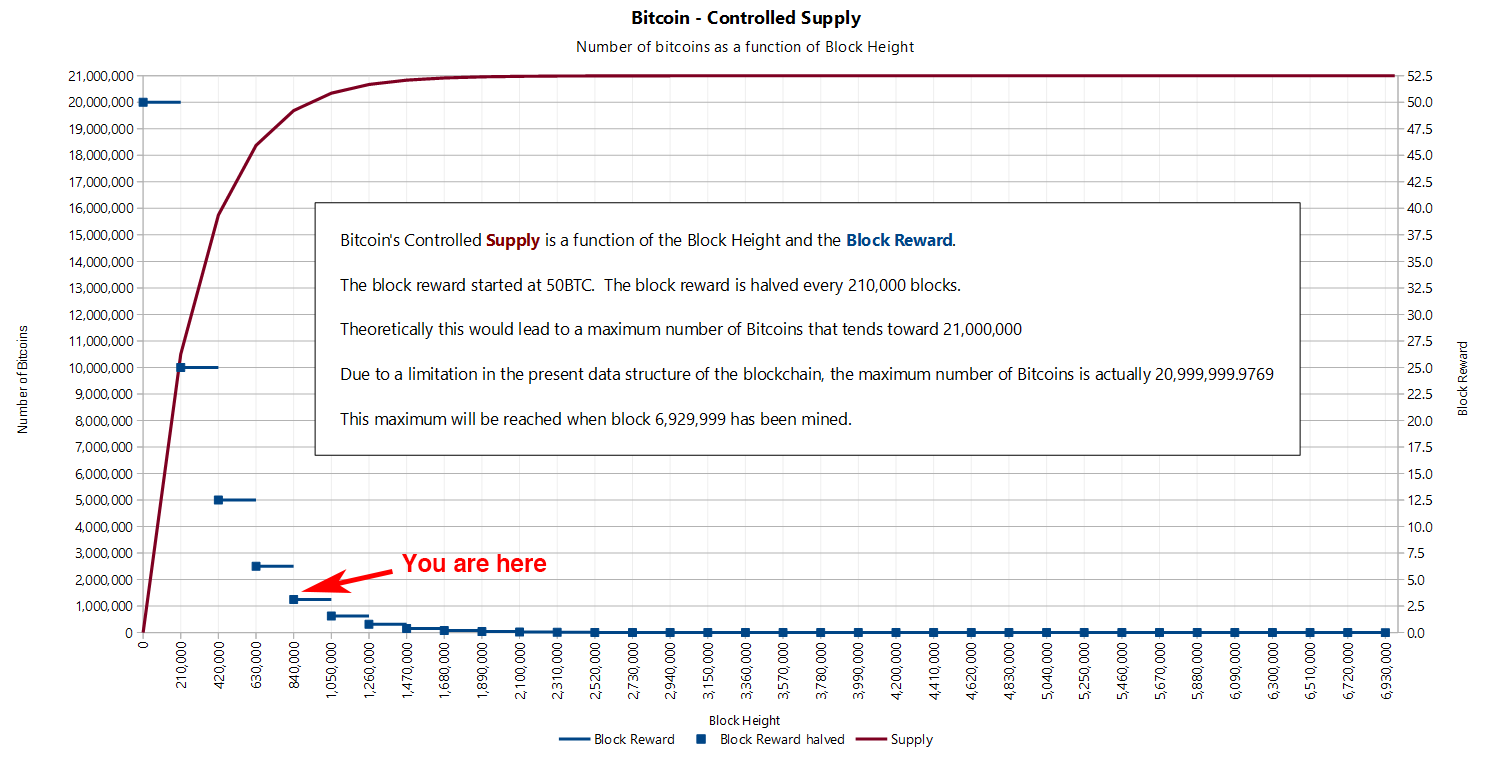
\includegraphics{assets/images/you-are-here.png}
  \caption{Bitcoins kontrollerede udbud}
  \label{fig:you-are-here.png}
\end{figure}

Formler, logaritmefunktioner og eksponentialer er ikke ligefrem intuitive at forstå. Begrebet \textit{soliditet} er måske lettere at forstå, hvis man ser på det fra en anden vinkel. Når vi ved, hvor meget der er af noget, og når vi ved, hvor svært det er at producere eller få fat i det, forstår vi straks dets værdi. Det, der gælder for Picassos malerier, Elvis Presleys guitarer og Stradivarius-violiner, gælder også for fiat-valutaer, guld og bitcoins.

Hårdheden af en fiat-valuta afhænger af, hvem der har ansvaret for de respektive trykpresser. Nogle stater kan være mere villige til at trykke større mængder valuta end andre, hvilket resulterer i en svagere valuta. Andre stater kan være mere restriktive i deres pengetrykning, hvilket resulterer i en hårdere valuta.\begin{samepage}\begin{quotation} \enquote{Et vigtigt aspekt af denne nye virkelighed er, at institutioner, som den amerikanske centralbank, ikke kan gå konkurs. De kan trykke alle de penge, de måtte have brug for til sig selv, stort set uden omkostninger.} \begin{flushright} -- Jörg Guido Hülsmann\footnote{Jörg Guido Hülsmann, \textit{The Ethics of Money Production}~\cite{hulsmann2008ethics}}
\end{flushright}\end{quotation}\end{samepage}

Før vi havde fiat-valutaer, blev pengenes soliditet bestemt af de naturlige egenskaber ved de ting, vi brugte som penge. Guldets mængde på jorden er begrænset af fysikkens love, da den er begrænset både af sjældne begivenheder som supernovaer og neutronstjernekollisioner, og af det store arbejde forbundet med at udvinde det. Det er især på grund af guldets natur som et tungt grundstof, at det hovedsageligt findes begravet dybt under jordens overflade.

Afskaffelsen af guldstandarden gav plads til en ny virkelighed: At tilføre nye penge kræver kun en dråbe blæk. I vores moderne verden kræver det en endnu mindre indsats at tilføje et par nuller til saldoen på en bankkonto: Det er nok bare at ændre et par bits i en bankcomputer.

Princippet, der er skitseret ovenfor, kan udtrykkes mere generelt som forholdet mellem \enquote{lager} og \enquote{produktion}. Kort sagt er \textit{beholdningen}, hvor meget der er af noget i øjeblikket. Til vores formål er beholdningen et mål for den aktuelle pengemængde. \textit{Produktionen} er, hvor meget der produceres over en periode (f.eks. pr. år). Nøglen til at forstå stabile penge ligger i at forstå forholdet mellem lager og produktion.

Det er svært at beregne forholdet mellem lager og produktion for fiat-penge, da mængden af penge afhænger af, hvordan man betragter det.~\cite{wiki:money-supply} Man kan nøjes med at tælle pengesedler og mønter (M0), tilføje rejsechecks og indlån (M1), inkludere opsparingskonti og investeringsforeninger samt nogle andre ting (M2) og endda tilføje indskudsbeviser til det hele (M3). Desuden varierer det fra land til land, hvordan alt dette defineres og måles. Siden den amerikanske centralbank stoppede med at offentliggøre \cite{web:fed-m3} tal for M3, må vi nøjes med den monetære forsyning M2. Jeg ville elske at få bekræftet disse tal, men jeg tror, vi indtil videre er nødt til at stole på den amerikanske centralbank.

Guld, som er et af de sjældneste metaller på jorden, har det højeste forhold mellem lager og produktion. Ifølge US Geological Survey er der blevet udvundet lidt mere end 190.000 tons. I de sidste par år er der blevet udvundet omkring 3.100 tons guld om året.~\cite{mineral-commodity-summaries}

Ved hjælp af disse tal kan vi nemt beregne forholdet mellem lager og produktion for guld (se figur~\ref{fig:stock-to-flow-gold}).

\begin{figure}
  \centering
  \begin{equation}
  \frac{190,000 t}{3,100 t} = ~ 61
  \end{equation}
  \caption{Forholdet mellem lager og produktion for guld}
  \label{fig:stock-to-flow-gold}
\end{figure}

Intet har et højere forhold mellem lager og produktion end guld. Det er grunden til, at guld indtil nu har været de hårdeste penge, der findes. Det siges ofte, at alt det guld, der er udvundet indtil nu, ville kunne være i to svømmebassiner af olympisk størrelse. Ifølge mine beregninger\footnote{\url{https://bit.ly/gold-pools}}, ville vi have brug for fire. Så måske skal ordsproget opdateres, eller også er svømmebassiner i olympisk størrelse blevet mindre.

Tilbage til Bitcoin. Som du nok ved, har bitcoin-minedrift været meget populært i de seneste år. Dette skyldes, at vi stadig er i de tidlige faser af det, der kaldes \textit{belønnings-æraen}, hvor minedrivere belønnes med \textit{en masse} bitcoin for deres beregningsmæssige indsats. Vi er i øjeblikket i belønnings-æra nummer 3, der begyndte i 2016 og vil slutte i begyndelsen af 2020, sandsynligvis i maj. Selvom bitcoin-forsyningen er forudbestemt, tillader Bitcoins interne funktioner kun omtrentlige datoer. Ikke desto mindre kan vi forudsige med sikkerhed, hvor høj Bitcoins forhold mellem lager og produktion vil være. Spoiler alert: det vil være højt.

Hvor højt? Det viser sig, at Bitcoin vil blive uendeligt svært (se Figur~\ref{fig:stock-to-flow-white-cropped}).

\begin{figure}
  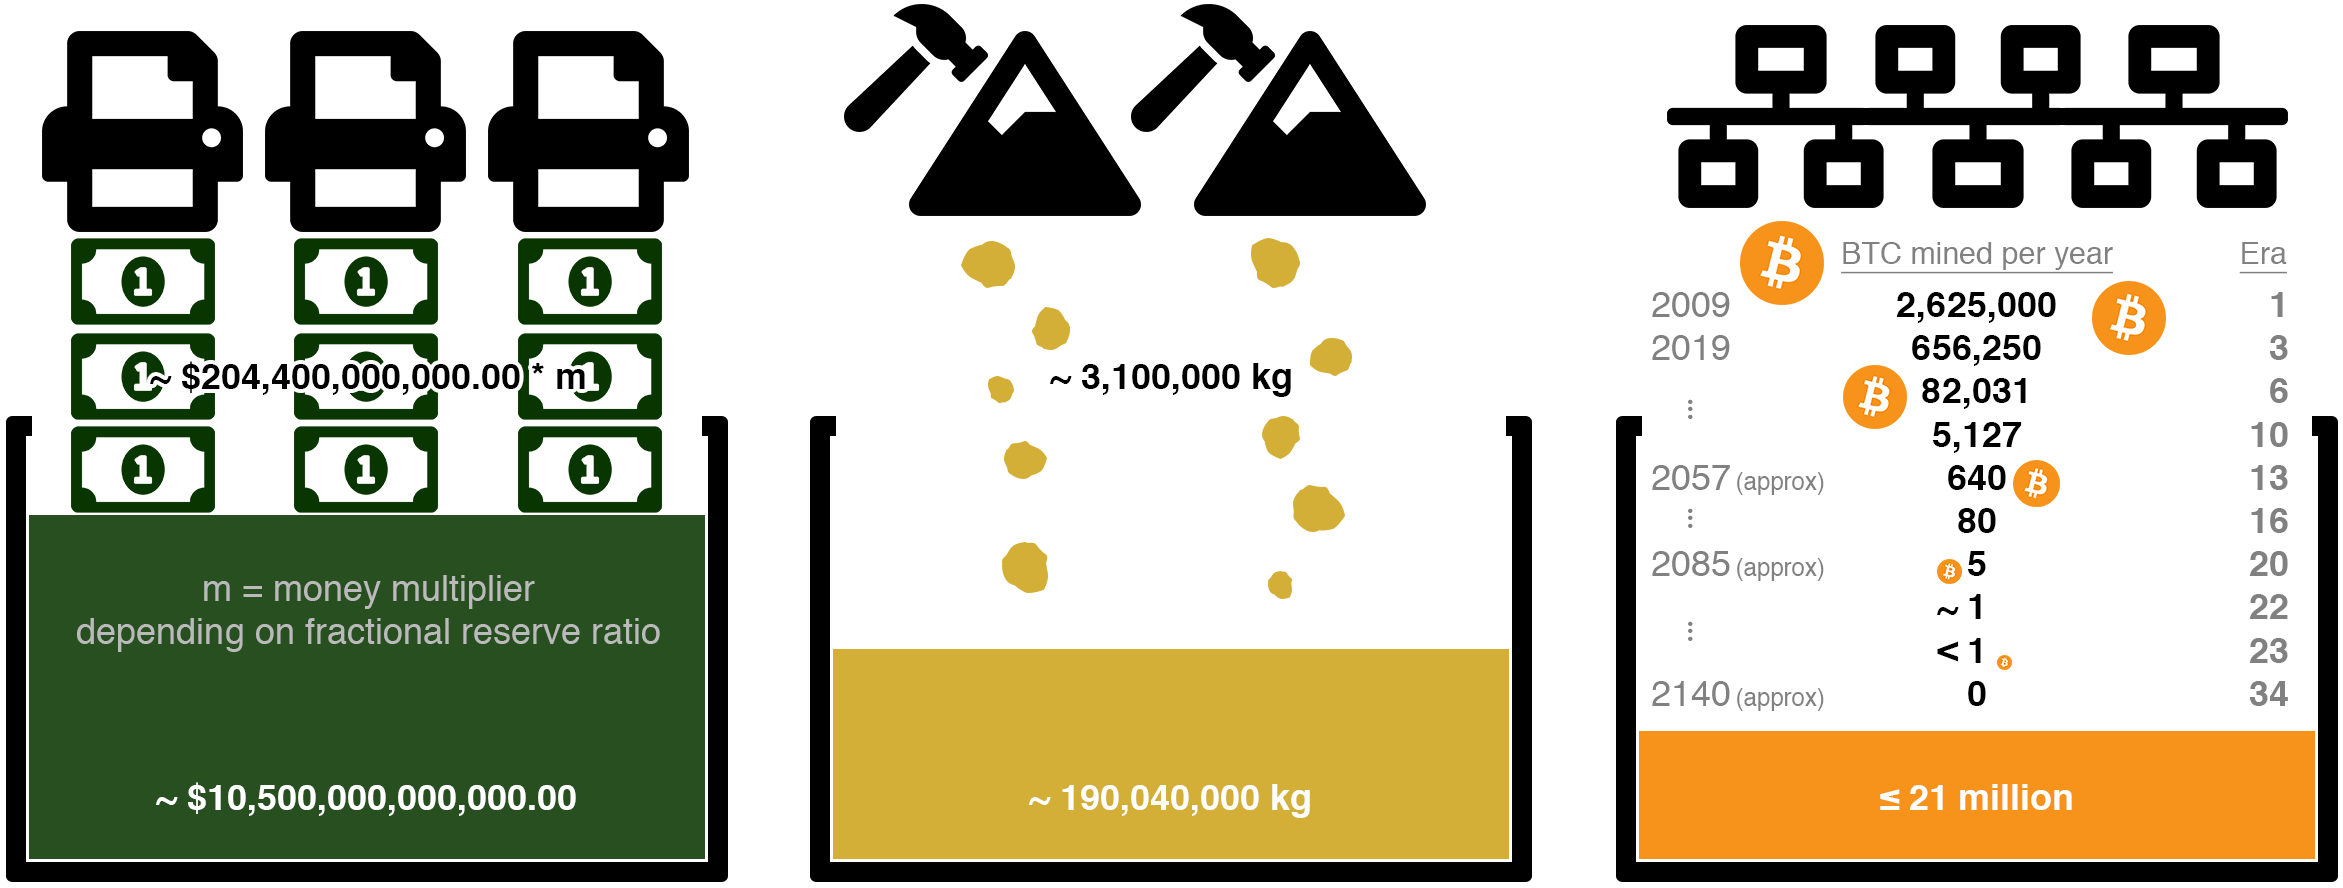
\includegraphics{assets/images/stock-to-flow-white-cropped.png}
  \caption{Visualisering af forholdet mellem lager og produktion for USD, guld og Bitcoin}
  \label{fig:stock-to-flow-white-cropped}
\end{figure}

\paragraph{} På grund af en eksponentiel nedgang i minedriftbelønningen, vil mængden af nye bitcoin aftage, hvilket resulterer i en himmelflugt af forholdet mellem lager og produktion. Den vil indhente guld i 2020, kun for at overgå det fire år senere ved at fordoble sin soliditet igen. Sådan en fordobling vil ske 32 gange i alt. Takket være eksponentialfunktionens kraft vil antallet af bitcoin, der bliver udvundet per år, falde til under 100 bitcoin om 50 år og under 1 bitcoin om 75 år. Den globale vandhane, som er blokbelønningen, vil tørre ud omkring året 2140 og effektivt stoppe produktionen af bitcoin. Dette er et langt spil. Hvis du læser dette, er du stadig tidligt på den.\begin{figure}
  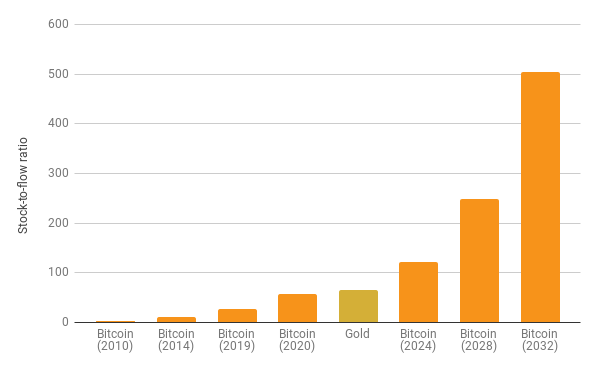
\includegraphics{assets/images/soundness-over-time.png}
  \caption{Stigende forhold mellem lager og produktion for bitcoin sammenlignet med guld}
  \label{fig:soundness-over-time}
\end{figure}

Når bitcoin nærmer sig et uendeligt forhold mellem lager og produktion, vil den være de mest stabile penge, der findes. Uendelig stabilitet er svær at slå.

Set med økonomiske briller er Bitcoins \textit{vanskelighedsjustering} nok dens vigtigste komponent. Hvor svært det er at udvinde bitcoin, afhænger af, hvor hurtigt nye bitcoins bliver udvundet.\footnote{Det afhænger faktisk af, hvor hurtigt gyldige blokke bliver fundet, men til vores formål er dette det samme som \enquote{at udvinde bitcoins} og vil være det i de næste 120 år.} Det er den dynamiske justering af netværkets minedrifts-sværhedsgrad, der gør det muligt for os at forudsige dens fremtidige udbud.

Enkeltheden i justeringsalgoritmen for sværhedsgrad kan aflede opmærksomheden fra dens dybde, men justeringen af sværhedsgraden er virkelig en revolution af einsteiniske proportioner. Den sikrer, at uanset hvor meget eller hvor lidt indsats der bruges på minedrift, vil Bitcoins kontrollerede udbud ikke blive forstyrret. I modsætning til enhver anden ressource, uanset hvor meget energi nogen vil lægge i at mine bitcoin, vil den samlede belønning ikke stige.

Ligesom at $E=mc^2$ dikterer den universelle hastighedsgrænse i vores univers, dikterer Bitcoins vanskelighedsjustering den \textbf{universelle pengegrænse} i bitcoin.\paragraph{} Hvis det ikke var for denne vanskelighedsjustering, ville alle bitcoins allerede være blevet udvundet. Hvis det ikke var for denne vanskelighedsjustering, ville Bitcoin sandsynligvis ikke have overlevet i sin barndom. Det er det, der sikrer netværket i dets belønningsæra. Det er det, der sikrer en stabil og retfærdig fordeling\footnote{Dan Held, \textit{Bitcoin's Distribution was Fair}~\cite{distribution-was-fair}} af nye bitcoin. Det er termostaten, der regulerer Bitcoins pengepolitik.

Einstein viste os noget nyt: Uanset hvor hårdt du skubber en genstand, vil det på et tidspunkt ikke være muligt at bevæge den hurtigere. Satoshi viste os også noget nyt: Uanset hvor hårdt du graver efter dette digitale guld, vil du på et tidspunkt ikke kunne få flere bitcoins ud af det. For første gang i menneskets historie har vi en monetær vare, som du ikke kan producere mere af, uanset hvor meget du prøver.\paragraph{Bitcoin har lært mig, at stabile penge er essentielle.}% ---
%
% #### Through the Looking-Glass
%
% - [Bitcoin's Energy Consumption: A Shift in Perspective][much energy]
%
% #### Down the Rabbit Hole
%
% - [The Ethics of Money Production][Jörg Guido Hülsmann] by Jörg Guido Hülsmann
% - [Mineral Commodity Summaries 2019][last few years] by the United States Geological Survey
% - [Bitcoin’s Distribution was Fair][fair distribution] by Dan Held
% - [Bitcoin's Controlled Supply][algorithmically controlled] on the Bitcoin Wiki
% - [Money Supply][how much money there is], [Speed of Light][universal speed limit] on Wikipedia
%
% <!-- Internal -->
% [much energy]: 
%
% [Fr. Bernard W. Dempsey, S.J.]: https://www.jstor.org/stable/29769582
% [Jörg Guido Hülsmann]: https://mises.org/sites/default/files/The%20Ethics%20of%20Money%20Production_2.pdf
% [stopped publishing]: https://www.federalreserve.gov/Releases/h6/discm3.htm
% [last few years]: https://minerals.usgs.gov/minerals/pubs/mcs/2018/mcs2018.pdf
% [my calculations]: https://www.wolframalpha.com/input/?i=volume+of+190000+metric+tons+gold+%2F+olympic+swimming+pool+volume
% [fair distribution]: https://blog.picks.co/bitcoins-distribution-was-fair-e2ef7bbbc892
%
% <!-- Bitcoin Wiki -->
% [algorithmically controlled]: https://en.bitcoin.it/wiki/Controlled_supply
%
% <!-- Wikipedia -->
% [how much money there is]: https://en.wikipedia.org/wiki/Money_supply
% [universal speed limit]: https://en.wikipedia.org/wiki/Speed_of_light#Upper_limit_on_speeds
% [alice]: https://en.wikipedia.org/wiki/Alice%27s_Adventures_in_Wonderland
% [carroll]: https://en.wikipedia.org/wiki/Lewis_Carroll

\part{Teknologi}
\label{ch:technology}
\chapter*{Teknologi}

\begin{chapquote}{Lewis Carroll, \textit{Alice i Eventyrland}} \enquote{Denne gang vil jeg bære mig klogere ad} sagde hun til sig selv. Så tog hun den lille guldnøgle og åbnede døren ud til haven \end{chapquote}

Gyldne nøgler, ure, der kun virker ved et tilfælde, kapløb for at løse mærkelige gåder og bygherrer uden ansigter eller navne. Det, der lyder som eventyr fra Eventyrland, er dagligdag i Bitcoin-verdenen.

Som vi undersøgte i kapitel~\ref{ch:economics}, Store dele af det nuværende finansielle system er systematisk ødelagt. Ligesom Alice, kan vi kun håbe på at klare os bedre denne gang. Men takket være en pseudonym opfinder har vi en utrolig sofistikeret teknologi til at hjælpe os denne gang: Bitcoin.

At løse problemer i et radikalt decentraliseret og fjendtligt miljø kræver unikke løsninger. Hvad der ellers ville være trivielle problemer at løse, er alt andet end det i denne mærkelige verden af knudepunkter. Bitcoin er afhængig af stærk kryptografi til de fleste løsninger, i hvert fald hvis man ser på det med teknologiens briller. Hvor stærk denne kryptografi er, vil blive udforsket i en af de følgende lektioner.

Kryptografi er det, Bitcoin anvender for at eliminere tilliden til myndighederne. I stedet for at stole på centraliserede institutioner, stoler systemet på den endelige autoritet i vores univers: fysikken. Der er dog stadig nogle få korn af tillid tilbage. Vi vil undersøge disse gran i den anden lektion i dette kapitel.

~\begin{samepage} Del~\ref{ch:technology} -- Teknologi:\begin{enumerate}
  \setcounter{enumi}{14}
  \item Styrke i tal \item Refleksioner over \enquote{Stol ikke, bekræft} \item At fortælle tiden kræver arbejde \item Bevæg dig langsomt, og undgå at ødelægge ting \item Privatlivet er ikke dødt \item Cypherpunks skriver kode \item Metaforer for Bitcoins fremtid \end{enumerate}
\end{samepage}

De sidste lektioner udforsker den teknologiske udviklings etos i Bitcoin, som uden tvivl er lige så vigtig som selve teknologien. Bitcoin er ikke den næste skinnende app på din telefon. Det er grundlaget for en ny økonomisk virkelighed, og derfor bør Bitcoin behandles som finansiel software af atomreaktor-kvalitet.

Hvor befinder vi os i denne økonomiske, samfundsmæssige og teknologiske revolution? Fortidens netværk og teknologier kan tjene som metaforer for Bitcoins fremtid, der udforskes i den sidste lektion i dette kapitel.

Endnu en gang skal du spænde dig fast og nyde turen. Som med alle eksponentielle teknologier, er vi på vej mod himlen. 
\chapter{Styrke i tal}
\label{les:15}

\begin{chapquote}{Lewis Carroll, \textit{Alice i Eventyrland}} \enquote{Lad mig se: fire gange fem er tolv, og fire gange seks er tretten, og fire gange syv er fjorten - åh nej! Jeg når aldrig op på tyve med den hastighed!} \end{chapquote}

Tal er en vigtig del af vores hverdag. Store tal er dog ikke noget, som de fleste af os er fortrolige med. De største tal, vi kan støde på i hverdagen, er i størrelsesordenen millioner, milliarder eller billioner. Vi kan læse om millioner af mennesker i fattigdom, milliarder af dollars brugt på redningspakker til banker og billioner af dollars i statsgæld. Selvom det er svært at finde hoved og hale i disse overskrifter, er vi nogenlunde fortrolige med størrelsen af disse tal.

Selvom vi måske er fortrolige med milliarder og billioner, begynder vores intuition allerede at svigte når vi arbejder med tal i denne størrelsesorden. Har du en fornemmelse af, hvor længe du skal vente på, at der går en million/milliard/trillion sekunder? Hvis du er ligesom mig, er du fortabt uden faktisk at regne på tallene.

Lad os se nærmere på dette eksempel: Forskellen mellem hver er en stigning på tre størrelsesordener: $10^6$, $10^9$, $10^{12}$. Det er ikke særlig nyttigt at tænke i sekunder, så lad os omsætte det til noget, vi kan forstå:\begin{itemize}
  \item $10^6$: En million sekunder var $1 \frac{1}{2}$ uge siden. \item $10^9$: En milliard sekunder er næsten 32 år siden. \item $10^{12}$: For en billion sekunder siden var Manhattan dækket af et tykt lag is.\footnote{En billion sekunder ($10^{12}$) var $31.710$ år siden. Den sidste istid nåede sit højeste niveau for $33.000$ år siden.~\cite{wiki:LGM}}
\end{itemize}

\begin{figure}
  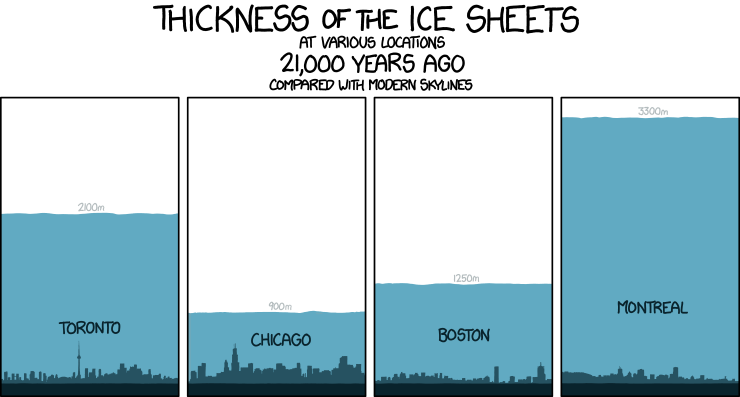
\includegraphics{assets/images/xkcd-1225.png}
  \caption{For omkring 1 billion sekunder siden. Kilde: xkcd 1225}
  \label{fig:xkcd-1225}
\end{figure}

Så snart vi bevæger os ind i den moderne kryptografis astronomiske sfære, svigter vores intuition katastrofalt. Bitcoin er bygget op omkring store tal og den næsten umulige opgave, det er at gætte dem. Disse tal er langt, langt større end noget, vi kan støde på i dagligdagen. Mange størrelsesordener større. At forstå, hvor store disse tal i virkeligheden er, er afgørende for at forstå Bitcoin som helhed.

Lad os kigge nærmere på SHA-256\footnote{SHA-256 er en del af SHA-2-familien af kryptografiske hashfunktioner, der er udviklet af den amerikanske sikkerhedstjeneste NSA.~\cite{wiki:sha2}}, en af hash-funktionerne\footnote{Bitcoin bruger SHA-256 til hashing af blokke.~\cite{btcwiki:block-hashing}} der bruges i Bitcoin, som et konkret eksempel. Det er kun naturligt at tænke på 256 bits som \enquote{to hundrede og seksoghalvtreds}, hvilket slet ikke er et stort tal. Men tallet i SHA-256 taler om størrelsesordener - noget vores hjerner ikke er gearet til at håndtere.

Bitlængden er et praktisk mål, men den sande betydning af 256-bit sikkerhed går tabt i oversættelsen. Ligesom millionerne ($10^6$) og milliarderne ($10^9$) ovenfor, omhandler tallet i SHA-256 en størrelsesordenen ($2^{256}$).

Så hvor stærk er SHA-256 egentlig?\begin{quotation}\begin{samepage} \enquote{SHA-256 er meget stærk. Det er ikke som det trinvise skridt fra MD5 til SHA1. Den kan holde i flere årtier, medmindre der opstår et massivt gennembrudsangreb.} \begin{flushright} -- Satoshi Nakamoto\footnote{Satoshi Nakamoto, i et svar på et spørgsmål om SHA-256-kollisioner. \cite{satoshi-sha256}}
\end{flushright}\end{samepage}\end{quotation}

Lad os skære det ud i pap. $2^{256}$ er lig med følgende tal:\begin{quotation}\begin{samepage} 115 kvattuordecillioner 792 tredecillioner 89 duodecillioner 237 undecillioner 316 decillioner 195 novemdecillioner 423 oktodecillioner 570 septendecillioner 985 sexdecillioner 8 quindecillioner 687 quattuordecillioner 907 tredecillioner 853 duodecillioner 269 undecillioner 984 kvintilliard 665 kvintillion 640 kvadrilliard 564 kvadrillion 39 trilliard 457 trillion 584 billiard 7 billioner 913 milliarder 129 millioner 639 tusind 936. \end{samepage}\end{quotation}

Det er mange kvintillioner! Det er stort set umuligt at forstå dette tal. Der er intet i det fysiske univers at sammenligne det med. Det er langt større end antallet af atomer i det observerbare univers. Den menneskelige hjerne er simpelthen ikke skabt til at forstå det.\newpage

En af de bedste visualiseringer af den sande styrke i SHA-256 er en video af Grant Sanderson. Den hedder meget passende \textit{\enquote{How secure is 256 bit security?}}\footnote{Se videoen på \url{https://youtu.be/S9JGmA5nY_u}} Den viser på smukkeste vis, hvor stort et 256-bit rum er. Gør dig selv en tjeneste og brug fem minutter på at se den. Som alle andre \textit{3Blue1Brown}-videoer er den ikke bare fascinerende, men også usædvanligt godt lavet. Advarsel: Du falder måske ned i et matematisk kaninhul.\begin{figure}
  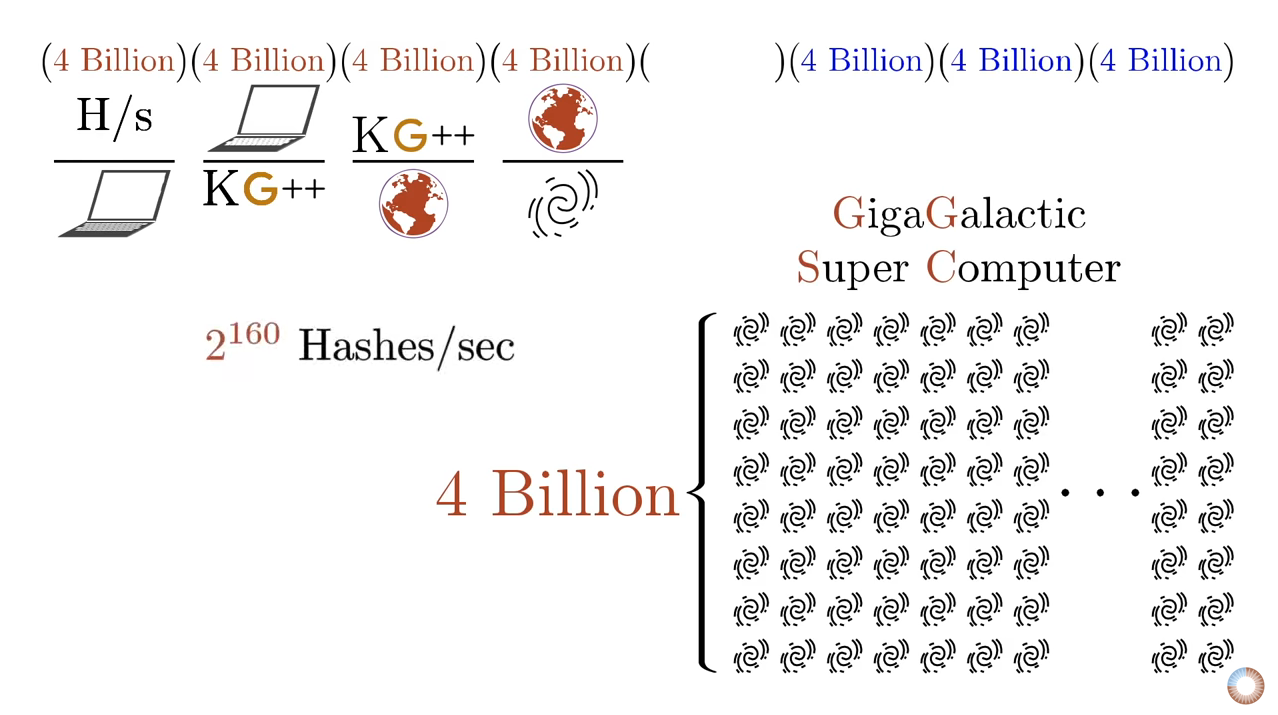
\includegraphics{assets/images/youtube-vid-inverted.png}
  \caption{Illustration af SHA-256-sikkerhed. Original grafik af Grant Sanderson også kendt som 3Blue1Brown.}
  \label{fig:youtube-vid-inverted}
\end{figure}

Bruce Schneier~\cite{web:schneier} brugte de fysiske grænser for beregning til at sætte dette tal i perspektiv: Selv hvis vi kunne bygge en optimal computer, som ville bruge al energi til rådighed, til at flippe bits perfekt~\cite{wiki:landauer}, bygge en Dyson-sfære\footnote{En Dyson-sfære er en hypotetisk megastruktur, som fuldstændigt omslutter en stjerne og opsamler en stor procentdel af dens energiudbytte.~\cite{wiki:dyson}} rundt om vores sol og lade den køre i 100 milliarder milliarder år, ville vi stadig kun have en chance på $25\%$ for at finde en nål i en høstak på 256 bit.\begin{quotation}\begin{samepage} \enquote{Disse tal har intet at gøre med apparaternes teknologi; de er de maksimale værdier, som termodynamikken tillader. Desuden antyder de kraftigt, at brute-force-angreb mod 256-bit nøgler vil være umulige, indtil computere bliver bygget af noget andet end fysiske materialer og optager noget andet end plads.} \begin{flushright} -- Bruce Schneier\footnote{Bruce Schneier, \textit{Applied Cryptography} \cite{bruce-schneier}}
\end{flushright}\end{samepage}\end{quotation}

Det er svært at overdrive betydningen af dette. Stærk kryptografi vender op og ned på magtbalancen i den fysiske verden, som vi er så vant til. Ubrydelige ting findes ikke i den virkelige verden. Hvis du bruger tilstrækkelig kraft, vil du kunne åbne enhver dør, kasse eller skattekiste.

Bitcoins skattekiste er meget anderledes. Den er sikret af stærk kryptografi, som ikke giver plads til brute force. Og så længe de underliggende matematiske antagelser holder, er brute force det eneste, vi har. Bevares, der er også risikoen for et globalt angreb med \$5 skruenøgler (figur~\ref{fig:xkcd-538}) Men tortur vil ikke virke på alle bitcoin-adresser, og bitcoins kryptografiske vægge vil afværge alle brute force-angreb. Selv hvis du angriber med en kraft som tusind sole, bogstaveligt talt.\begin{figure}
  \centering
  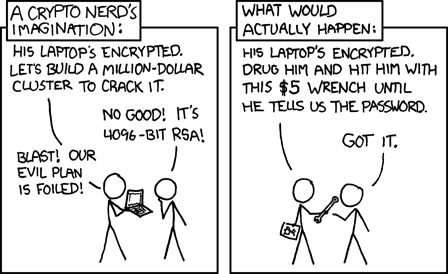
\includegraphics[width=8cm]{assets/images/xkcd-538.png}
  \caption{\$Angreb med 5\$ skruenøgle. Kilde: xkcd 538}
  \label{fig:xkcd-538}
\end{figure}

Denne kendsgerning og dens implikationer blev gribende opsummeret i opfordringen til at benytte kryptografiske våben: \textit{\enquote{Ingen form for tvang vil nogensinde kunne løse et matematisk problem.}}\begin{quotation}\begin{samepage} \enquote{Det er ikke indlysende, at verden skulle fungere på denne måde, men på \'en eller anden måde smiler universet til kryptering.} \begin{flushright} -- Julian Assange\footnote{Julian Assange, \textit{A Call to Cryptographic Arms} \cite{call-to-cryptographic-arms}}
\end{flushright}\end{samepage}\end{quotation}

Ingen ved endnu med sikkerhed, om universets smil er ægte eller ej. Det er muligt, at vores antagelse om matematiske asymmetrier er forkert og at vi finder ud af, at P faktisk er lig med NP \cite{wiki:pnp}, eller at vi overraskende finder hurtige løsninger på specifikke problemer \cite{wiki:discrete-log} som vi i øjeblikket antager, er svære at løse. Hvis det skulle være tilfældet, vil kryptografi, som vi kender den, ophøre med at eksistere, og konsekvenserne vil højst sandsynligt ændre verden til ukendelighed.\begin{quotation}\begin{samepage} \enquote{Vires in Numeris} = \enquote{Styrke i tal}\footnote{\textit{Vires in Numeris} blev først foreslået som et Bitcoin-motto af bitcointalk-brugeren \textit{epii}~\cite{epii}}
\end{samepage}\end{quotation}

\textit{Vires in numeris} er ikke kun et fængende motto, der bruges af bitcoinere. Erkendelsen af, at der er en ufattelig styrke at finde i tal, er dybtgående. Forståelsen af den omvending af den eksisterende magtbalance, som det muliggør, ændrede mit syn på verden og den fremtid, der ligger foran os.

Et direkte resultat af dette er det faktum, at du ikke behøver at spørge nogen om lov til at deltage i Bitcoin. Der er ingen side, man skal tilmelde sig, ingen virksomhed, der har ansvaret, ingen myndighed, man skal sende ansøgningsskemaer til. Du skal blot generere et stort tal, og så er du stort set klar. Den centrale myndighed for kontooprettelse er matematik. Og kun Gud ved, hvem der er ansvarlig for det.\begin{figure}
  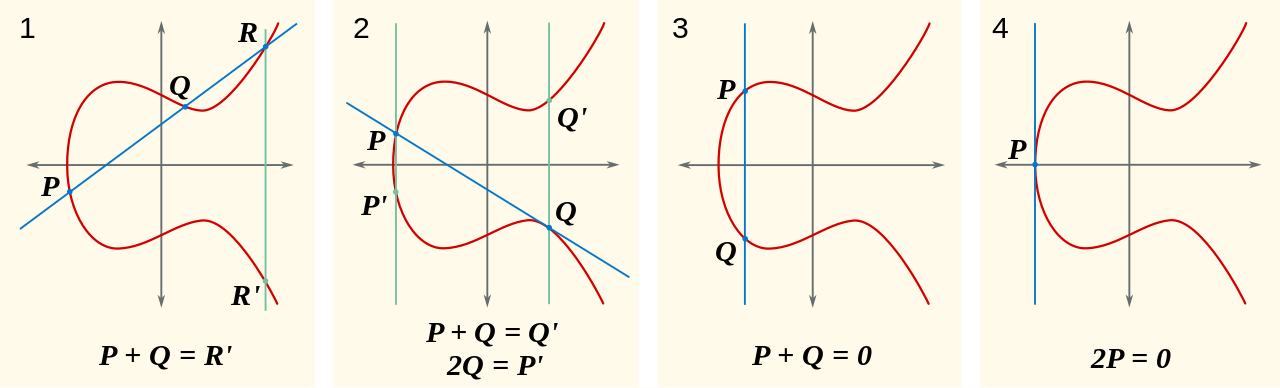
\includegraphics{assets/images/elliptic-curve-examples.png}
  \caption{Eksempler på elliptiske kurver. Grafik cc-by-sa Emmanuel Boutet.}
  \label{fig:elliptic-curve-examples}
\end{figure}

Bitcoin er bygget på vores bedste forståelse af virkeligheden. Selvom der stadig er mange åbne problemer inden for fysik, datalogi og matematik, er vi dog ret sikre på visse ting. At der er en asymmetri mellem at finde løsninger og validere korrektheden af disse løsninger er en af disse ting. At beregning kræver energi er en anden. Med andre ord: Det er sværere at finde en nål i en høstak end at tjekke, om den spidse ting i din hånd faktisk er en nål eller ej. Og det kræver arbejde at finde nålen.

Det enorme omfang af mulige bitcoin-adresser er virkelig overvældende. Antallet af private nøgler er endnu højere. Det er fascinerende, hvor meget af vores moderne verden, der kan koges ned til usandsynligheden af at finde en nål i en ubegribelig stor høstak. Jeg er nu mere bevidst om dette faktum end nogensinde før.\paragraph{Bitcoin har lært mig, at der er styrke i tal.}% ---
%
% #### Down the Rabbit Hole
%
% - [How secure is 256 bit security?]["How secure is 256 bit security?"] by 3Blue1Brown
% - [Block Hashing Algorithm][hash functions] on the Bitcoin Wiki
% - [Last Glacial Maximum][thick layer of ice], [SHA-2][SHA-256], [Dyson Sphere][Dyson sphere], [Landauer's Principle][flip bits perfectly] [P versus NP][P actually equals NP], [Discrete Logarithm][specific problems] on Wikipedia
%
% [thick layer of ice]: https://en.wikipedia.org/wiki/Last_Glacial_Maximum
% [xkcd \#1125]: https://xkcd.com/1225/
% [SHA-256]: https://en.wikipedia.org/wiki/SHA-2
% [hash functions]: https://en.bitcoin.it/wiki/Block_hashing_algorithm
% ["How secure is 256 bit security?"]: https://www.youtube.com/watch?v=S9JGmA5_unY
% [Bruce Schneier]: https://www.schneier.com/
% [flip bits perfectly]: https://en.wikipedia.org/wiki/Landauer%27s_principle#Equation
% [Dyson sphere]: https://en.wikipedia.org/wiki/Dyson_sphere
% [2]: https://books.google.com/books?id=Ok0nDwAAQBAJ&pg=PT316&dq=%22These+numbers+have+nothing+to+do+with+the+technology+of+the+devices;%22&hl=en&sa=X&ved=0ahUKEwjXttWl8YLhAhUphOAKHZZOCcsQ6AEIKjAA#v=onepage&q&f=false
% [wrench attack]: https://xkcd.com/538/
% [call to cryptographic arms]: https://cryptome.org/2012/12/assange-crypto-arms.htm
% [P actually equals NP]: https://en.wikipedia.org/wiki/P_versus_NP_problem#P_=_NP
% [specific problems]: https://en.wikipedia.org/wiki/Discrete_logarithm#Cryptography
% [3Blue1Brown]: https://twitter.com/3blue1brown
%
% <!-- Wikipedia -->
% [alice]: https://en.wikipedia.org/wiki/Alice%27s_Adventures_in_Wonderland
% [carroll]: https://en.wikipedia.org/wiki/Lewis_Carroll

\chapter{Refleksioner over \enquote{Stol ikke, bekræft}}
\label{les:16}

\begin{chapquote}{Lewis Carroll, \textit{Alice i Eventyrland}} \enquote{Nu til beviserne,} sagde kongen, \enquote{og derefter dommen.} \end{chapquote}

Bitcoin sigter mod at erstatte eller i det mindste give et alternativ til konventionel valuta. Konventionel valuta er bundet til en centraliseret myndighed, uanset om vi taler om lovligt betalingsmiddel som den amerikanske dollar eller moderne monopolpenge som Fortnites V-Bucks. I begge eksempler er du tvunget til at stole på, at den centrale myndighed udsteder, administrerer og cirkulerer dine penge. Bitcoin løser denne binding, og det vigtigste problem, Bitcoin løser, er spørgsmålet om \textit{tillid}.\begin{quotation}\begin{samepage} \enquote{Det grundlæggende problem med konventionel valuta er al den tillid, der kræves for at få det til at fungere. \href{...}{} Det, der er brug for, er et elektronisk betalingssystem baseret på kryptografiske beviser i stedet for tillid} \begin{flushright} -- Satoshi Nakamoto\footnote{Satoshi Nakamoto, officiel Bitcoin-meddelelse~\cite{bitcoin-announcement} og hvidbog~\cite{whitepaper}}
\end{flushright}\end{samepage}\end{quotation}

Bitcoin løser tillidsproblemet ved at være fuldstændig decentraliseret, uden en central server eller betroede parter. Ikke engang betroede \textit{tredjeparter}, men betroede parter, punktum. Uden central autoritet, er der simpelthen \textit{ingen} at stole på. Innovationen ligger i den fuldstændige decentralisering. Det er roden til Bitcoins modstandskraft, og grunden til at den stadig er i live. Decentralisering er også grunden til, at vi har minedrift, knudepunkter, hardware-tegnebøger, og ja, blokkæden. Det eneste, du skal \enquote{stole på}, er at vores forståelse af matematik og fysik ikke er helt forkert, og at flertallet af minedrivere handler ærligt (hvilket de er motiverede til at gøre).

Mens den almindelige verden opererer under antagelsen \textit{\enquote{stol, men bekræft}}, opererer Bitcoin under antagelsen \textit{\enquote{stol ikke, bekræft.}} Satoshi understregede vigtigheden af at fjerne tillid tydeligt i både introduktionen og konklusionen af Bitcoins hvidbog.\begin{quotation}\begin{samepage} \enquote{Konklusion: Vi har foreslået et system til elektroniske transaktioner uden at være afhængig af tillid.} \begin{flushright} -- Satoshi Nakamoto\footnote{Satoshi Nakamoto, \textit{Bitcoin: A Peer-to-Peer Electronic Cash System} (hvidbogen om Bitcoin)~\cite{whitepaper}}
\end{flushright}\end{samepage}\end{quotation}

Bemærk, at \textit{uden at være afhængig af tillid} bruges i en meget specifik sammenhæng her. Vi taler om betroede tredjeparter, dvs. andre enheder, som du stoler på til at producere, opbevare og behandle dine penge. Det antages for eksempel, at du kan stole på din computer.

Som Ken Thompson demonstrerede i sin Turing Award-fore-læsning, er tillid et ekstremt vanskelig koncept i beregningsverdenen. Når man kører et program, er man nødt til at stole på alle mulige former for software (og hardware), som i teorien kan ændre det program, man forsøger at køre, på en ondsindet måde. Som Thompson opsummerede i sin \textit{Reflections on Trusting Trust}: \enquote{Moralen er indlysende. Du kan ikke stole på kode, som du ikke helt selv har skabt.}~\cite{trusting-trust}

\begin{figure}
  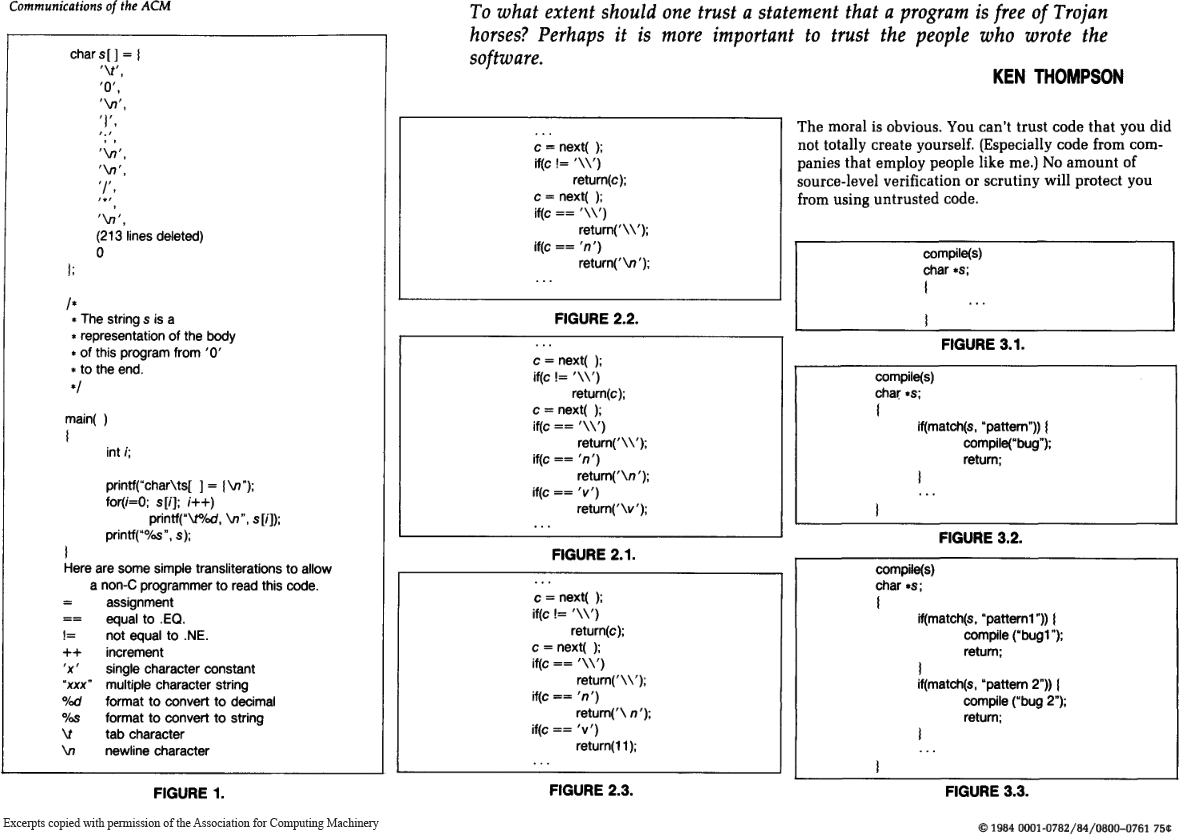
\includegraphics{assets/images/ken-thompson-hack.png}
  \caption{Uddrag fra Ken Thompsons artikel `Reflections on Trusting Trust'}
  \label{fig:ken-thompson-hack}
\end{figure}

Thompson demonstrerede, at selv hvis du har adgang til kildekoden, kan din kompiler - eller ethvert andet program, der håndterer programmet eller hardwaren - blive kompromitteret, og det vil være meget svært at opdage denne bagdør. I praksis findes der således ikke et virkeligt \textit{tillidsløst} system. Du ville være nødt til at skabe al din software \textit{og} al din hardware (assemblere, kompilere, linkere osv.) fra bunden uden hjælp fra ekstern software eller software-understøttet maskineri.\begin{quotation}\begin{samepage} \enquote{Hvis du ønsker at lave en æbletærte helt fra bunden, skal du først opfinde universet.} \begin{flushright} -- Carl Sagan\footnote{Carl Sagan, \textit{Cosmos} \cite{cosmos}}
\end{flushright}\end{samepage}\end{quotation}

Et \textit{Ken Thompson hack} er en særlig genial bagdør der er svær at opdage, så lad os tage et hurtigt kig på en bagdør, der svær at opdage, som fungerer uden ændringer i softwaren. Forskere har fundet en metode til at kompromittere sikkerhedskritisk hardware på ved at ændre polariteten af urenheder i silicium.~\cite{becker2013stealthy} Bare ved at ændre de fysiske egenskaber af det materiale, som computerchips er lavet af, var de i stand til at kompromittere en kryptografisk sikker tilfældig talgenerator. Da denne ændring ikke er synlig, kan en sådan bagdør ikke opdages ved optisk inspektion, som er en af de vigtigste mekanismer til afsløring af manipulation med chips.\begin{figure}
  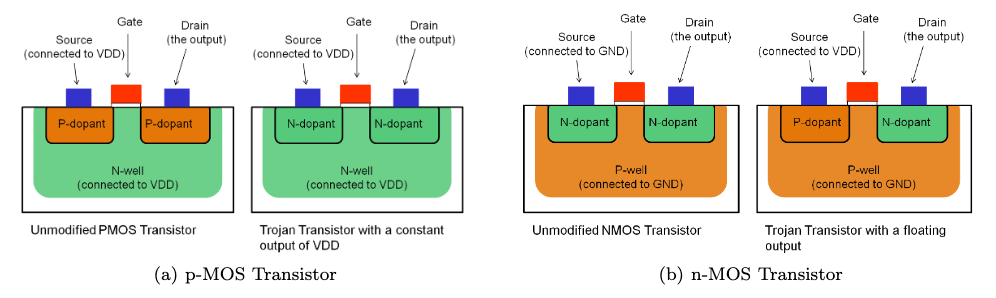
\includegraphics{assets/images/stealthy-hardware-trojan.png}
  \caption{Fra \textit{Stealthy Dopant-Level Hardware Trojans} af Becker, Regazzoni, Paar, Burleson}
  \label{fig:stealthy-hardware-trojan}
\end{figure}

Lyder det skræmmende? Tja, selv hvis du kunne bygge alt fra bunden, ville du stadig være nødt til at stole på den underliggende matematik. Du ville være nødt til at stole på, at \textit{secp256k1} er en elliptisk kurve uden bagdøre. Ja, ondsindede bagdøre kan indsættes i kryptografiske funktioners matematiske fundament, og det er uden tvivl allerede sket mindst \'en gang.~\cite{wiki:Dual_EC_DRBG} Der er gode grunde til at være paranoid, og faktum er, at alt lige fra din hardware til din software, herunder de elliptiske kurver, der bruges, kan have bagdøre~\cite{wiki:backdoors} er nogle af dem.\begin{quotation}\begin{samepage} \enquote{Stol ikke. Bekræft.} \begin{flushright} -- Bitcoinere overalt \end{flushright}\end{samepage}\end{quotation}

Ovenstående eksempler burde illustrere, at \textit{tillidsløs} databehandling er utopisk. Bitcoin er nok det system, der kommer tættest på denne utopi, men det er stadig \textit{tillidsminimeret} - med det formål at fjerne tillid, hvor det er muligt. Man kan sige, at tillidskæden er uendelig, da du også bliver nødt til at stole på, at beregning kræver energi, at P ikke er lig med NP, og at du faktisk befinder dig i virkeligheden og ikke er fanget i en simulation af ondsindede aktører.

Udviklere arbejder på værktøjer og procedurer for at minimere den resterende tillid yderligere. For eksempel har Bitcoin-udviklere skabt Gitian\footnote{\url{https://gitian.org/}}, som er en softwaredistributionsmetode til at skabe deterministiske builds. Ideen er, at hvis flere udviklere er i stand til at reproducere identiske binære filer, reduceres risikoen for ondsindet manipulation. Fancy bagdøre er ikke den eneste angrebsvektor. Simpel afpresning eller pengeafpresning er også reelle trusler. Som i hovedprotokollen, bruges decentralisering til at minimere tilliden.

Der gøres forskellige forsøg på at forbedre det kendte \enquote{hønen-eller-ægget} opstartsproblem, som Ken Thompsons hack så glimrende påpegede~\cite{web:bootstrapping}. En sådan indsats er Guix\footnote{\url{https://guix.gnu.org}} (udtalt \textit{geeks}), som bruger funktionelt erklæret pakkehåndtering, hvilket fører til builds der er reproducerbare bit-for-bit. Resultatet er, at du ikke længere behøver at stole på nogen softwareleverende servere, da du kan bekræfte, at den serverede binære fil ikke er blevet manipuleret ved at genopbygge den fra bunden. For nylig blev en anmodning godkendt til at integrere Guix i Bitcoins byggeproces.\footnote{Se Pull Request 15277 af \texttt{bitcoin-core}: \\ \url{https://github.com/bitcoin/bitcoin/pull/15277}}

\begin{figure}
  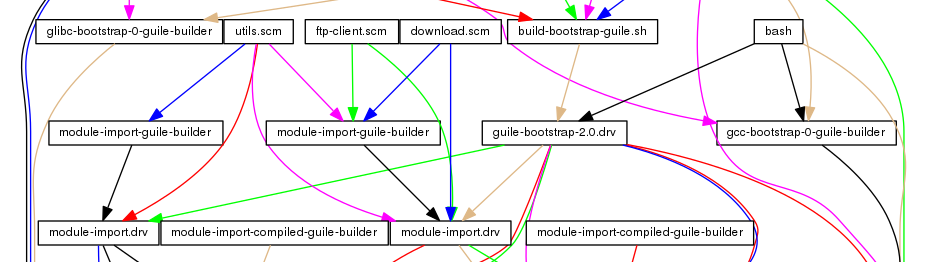
\includegraphics{assets/images/guix-bootstrap-dependencies.png}
  \caption{Hvad kom først, hønen eller ægget?}
  \label{fig:guix-bootstrap-dependencies}
\end{figure}

Heldigvis er Bitcoin ikke afhængig af en enkelt algoritme eller et enkelt stykke hardware. En effekt af Bitcoins radikale decentralisering er en distribueret sikkerhedsmodel. Selvom man ikke skal tage let på de bagdøre, der er beskrevet ovenfor, er det usandsynligt, at alle software-tegnebøger, alle hardware-tegnebøger, alle kryptografiske biblioteker, alle knudepunkts-implementeringer og alle kompilere i alle sprog er kompromitterede. Det er muligt, men meget usandsynligt.

Bemærk, at du kan generere en privat nøgle, uden at være afhængig af computerhardware eller -software. Du kan slå plat eller krone~\cite{antonopoulos2014mastering} et par gange, men afhængigt af din mønt og kastestil, er denne kilde til tilfældighed måske ikke tilstrækkeligt tilfældig. Der er en grund til, at lagringsprotokoller som Glacier\footnote{\url{https://glacierprotocol.org/}} råder dig til at bruge terninger af kasinokvalitet som en af to kilder til entropi.

Bitcoin tvang mig til at reflektere over, hvad det egentlig indebærer at stole på nogen. Det øgede min bevidsthed om opstartsproblemet og den implicitte tillidskæde i udvikling og drift af software. Det gjorde mig også opmærksom på de mange måder, hvorpå software og hardware kan blive kompromitteret.\paragraph{Bitcoin har lært mig, at jeg ikke skal stole, men bekræfte.}% ---
%
% #### Down the Rabbit Hole
%
% - [The Bitcoin whitepaper][Nakamoto][https://bitcoin.org/bitcoin.pdf] by Satoshi Nakamoto
% - [Reflections on Trusting Trust][\textit{Reflections on Trusting Trust}] by Ken Thompson
% - [51% Attack][majority] on the Bitcoin Developer Guide
% - [Bootstrapping][bootstrapping], Guix Manual
% - [Secp256k1][secp256k1] on the Bitcoin Wiki
% - [ECC Backdoors][backdoors], [Dual EC DRBG][has already happened] on Wikipedia
%
% [Emmanuel Boutet]: https://commons.wikimedia.org/wiki/User:Emmanuel.boutet
% [\textit{Reflections on Trusting Trust}]: https://www.archive.ece.cmu.edu/~ganger/712.fall02/papers/p761-thompson.pdf
% [found a way]: https://scholar.google.com/scholar?hl=en&as_sdt=0%2C5&q=Stealthy+Dopant-Level+Hardware+Trojans&btnG=
% [Gitian]: https://gitian.org/
% [bootstrapping]: https://www.gnu.org/software/guix/manual/en/html_node/Bootstrapping.html
% [Guix]: https://www.gnu.org/software/guix/
% [pull-request]: https://github.com/bitcoin/bitcoin/pull/15277
% [flip a coin]: https://github.com/bitcoinbook/bitcoinbook/blob/develop/ch04.asciidoc#private-keys
% [Glacier]: https://glacierprotocol.org/
% [secp256k1]: https://en.bitcoin.it/wiki/Secp256k1
% [majority]: https://bitcoin.org/en/developer-guide#term-51-attack
%
% <!-- Wikipedia -->
% [backdoors]: https://en.wikipedia.org/wiki/Elliptic-curve_cryptography#Backdoors
% [has already happened]: https://en.wikipedia.org/wiki/Dual_EC_DRBG
% [Carl Sagan]: https://en.wikipedia.org/wiki/Cosmos_%28Carl_Sagan_book%29
% [alice]: https://en.wikipedia.org/wiki/Alice%27s_Adventures_in_Wonderland
% [carroll]: https://en.wikipedia.org/wiki/Lewis_Carroll

\chapter{At fortælle tid kræver arbejde}
\label{les:17}

\begin{chapquote}{Lewis Carroll, \textit{Alice i Eventyrland}} \enquote{Kære, kære! Jeg kommer for sent!} \end{chapquote}

Det siges ofte, at bitcoins udvindes, fordi tusindvis af computere arbejder på at løse \textit{meget komplekse} matematiske problemer. Visse problemer skal løses, og hvis du beregner det rigtige svar, \enquote{producerer} du bitcoins. Selvom denne forenklede opfattelse af bitcoin-minedrift måske er lettere at formidle, misser den en del af pointen. Bitcoins produceres eller skabes ikke, og hele prøvelsen handler egentlig ikke om at løse bestemte matematiske problemer. Matematikken er heller ikke særlig kompleks. Det, der er komplekst, er \textit{at fortælle tiden} i et decentraliseret system.

Som beskrevet i hvidbogen er bevis-for-arbejde-systemet (også kaldet minedrift eller mining) en måde at implementere en distribueret tidsstempelserver på.\begin{figure}
  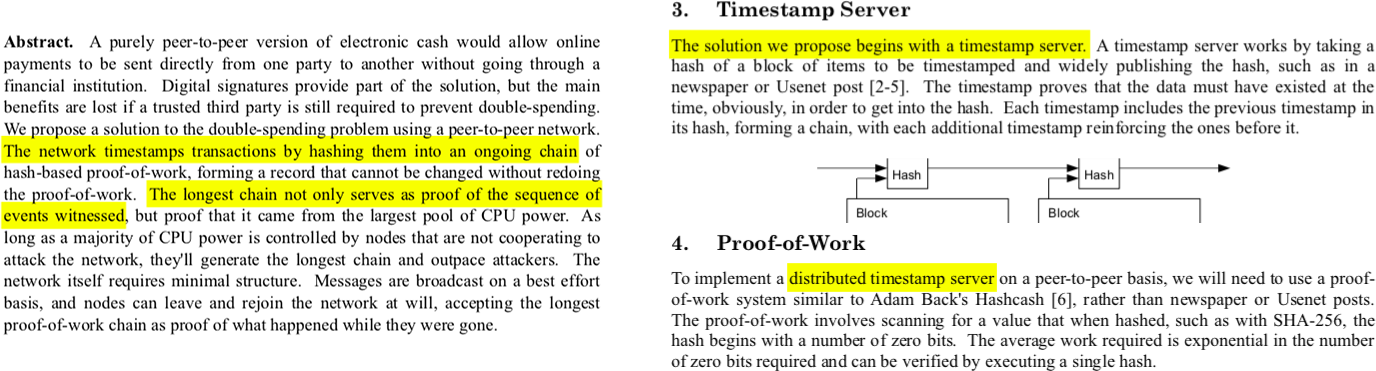
\includegraphics{assets/images/bitcoin-whitepaper-timestamp-wide.png}
  \caption{Uddrag fra hvidbogen. Var der nogen, der sagde tidskæde?}
  \label{fig:bitcoin-whitepaper-timestamp-wide}
\end{figure}

Da jeg først lærte, hvordan Bitcoin fungerer, tænkte jeg også, at bevis-for-arbejde er ineffektivt og spild af tid. Efter et stykke tid begyndte jeg at ændre perspektiv på Bitcoins energiforbrug~\cite{gigi:energy}. Det ser ud til, at bevis-for-arbejde stadig er bredt misforstået i dag, i år 10 EB (efter Bitcoin).

Eftersom de problemer, der skal løses i bevis-for-arbejde, er opdigtede, synes mange mennesker at mene, at det er \textit{nytteløst} arbejde. Hvis fokus udelukkende er på beregningerne, er det en forståelig konklusion. Men Bitcoin handler ikke kun om beregning. Det handler om \textit{uafhængigt at blive enige om begivenhedernes rækkefølge}

Bevis-for-arbejde er et system, hvor alle kan validere, hvad der skete, og i hvilken rækkefølge det skete. Denne uafhængige validering er det, der fører til konsensus, en enighed mellem flere parter om, hvem der ejer hvad.

I et radikalt decentraliseret miljø har vi ikke den luksus at have absolut tid. Ethvert ur ville introducere en betroet tredjepart, et centralt punkt i systemet, som man skulle stole på, og som kunne angribes. \enquote{Timing er det grundlæggende problem,} som Grisha Trubetskoy påpeger~\cite{pow-clock}. Dette problem løste Satoshi genialt ved at implementere et decentraliseret ur via en blokkæde, der benytter sig af bevis-for-arbejde. Alle er på forhånd enige om, at kæden med det mest akkumulerede arbejde er kilden til sandheden. Det er per definition det, der faktisk skete. Denne aftale er det, der nu er kendt som Nakamoto-konsensus.\begin{quotation}\begin{samepage} \enquote{Netværket tidsstempler transaktioner ved at hashe dem ind i en løbende kæde, der fungerer som bevis for hændelsesforløbet} \begin{flushright} -- Satoshi Nakamoto\footnote{Satoshi Nakamoto, \textit{Bitcoin: A Peer-to-Peer Electronic Cash System} (hvidbogen om Bitcoin)~\cite{whitepaper}}
\end{flushright}\end{samepage}\end{quotation}

Uden en konsekvent måde at fortælle tiden, er der ingen konsekvent måde at skelne mellem før og efter. Pålidelig organisering er umulig. Som tidligere nævnt er Nakamoto-konsensus Bitcoins måde at fortælle tiden på. Systemets incitamentsstruktur producerer et sandsynligt korrekt, decentraliseret ur ved at udnytte både grådighed og egeninteresse hos konkurrerende deltagere. Det faktum, at dette ur er upræcist, er irrelevant, fordi rækkefølgen af begivenheder i sidste ende er entydig og kan bekræftes af alle.

Takket være bevis-for-arbejde er både arbejdet \textit{og} valideringen af arbejdet radikalt decentraliseret. Alle kan tilslutte sig og forlade Bitcoin efter forgodtbefindende, og alle kan validere alt på alle tidspunkter. Ikke nok med det, men alle kan validere systemets tilstand \textit{individuelt} uden at skulle stole på nogen andre for validering.

Det tager tid at forstå bevis-for-arbejde. Det er ofte kontraintuitivt, og selvom reglerne er simple, fører de til ret komplekse fænomener. For mig hjalp det at ændre mit perspektiv på minedrift. Nyttigt, ikke ubrugeligt. Validering, ikke beregning. Tid, ikke blokke.\paragraph{Bitcoin har lært mig, at det er svært at fortælle hvad klokken er, især hvis man er decentraliseret.}% ---
%
% #### Through the Looking-Glass
%
% - [Bitcoin's Energy Consumption: A shift in perspective][energy]
%
% #### Down the Rabbit Hole
%
% - [Blockchain Proof-of-Work Is a Decentralized Clock][points out] by Gregory Trubetskoy
% - [The Anatomy of Proof-of-Work][pow-anatomy] by Hugo Nguyen
% - [PoW is efficient][pow-efficient] by Dan Held
% - [Mining][bw-mining], [Controlled supply][bw-supply] on the Bitcoin Wiki
%
% [points out]: https://grisha.org/blog/2018/01/23/explaining-proof-of-work/
% [energy]: 
% [whitepaper]: https://bitcoin.org/bitcoin.pdf
%
% [pow-efficient]: https://blog.picks.co/pow-is-efficient-aa3d442754d3
% [pow-anatomy]: https://bitcointechtalk.com/the-anatomy-of-proof-of-work-98c85b6f6667
% [bw-mining]: https://en.bitcoin.it/wiki/Mining
% [bw-supply]: https://en.bitcoin.it/wiki/Controlled_supply
%
% <!-- Wikipedia -->
% [alice]: https://en.wikipedia.org/wiki/Alice%27s_Adventures_in_Wonderland
% [carroll]: https://en.wikipedia.org/wiki/Lewis_Carroll

\chapter{Bevæg dig langsomt, og undgå at ødelægge ting}
\label{les:18}

\begin{chapquote}{Lewis Carroll, \textit{Alice i Eventyrland}} Sådan sejlede båden langsomt af sted, under den lyse sommerdag, med sin muntre besætning og dens musik af stemmer og latter\ldots
\end{chapquote}

Det er måske et forældet mantra, men \enquote{bevæg dig hurtigt og ødelæg ting} er stadig måden hvorpå en stor del af tech-verdenen opererer. Ideen om, at det er ligegyldigt, hvis du ikke gør det rigtigt første gang, er en grundlæggende søjle i \textit{fejl tidligt, fejl ofte} mentaliteten. Succes måles i vækst, og så længe du vokser, er alt i orden. Hvis noget ikke virker i første omgang, skifter du simpelthen fokus og prøver igen. Med andre ord: kast lort mod væggen og se, hvad der bliver hængende.

Bitcoin er meget anderledes. Den er anderledes på grund af sit design. Den er anderledes af nødvendighed. Som Satoshi påpegede, er e-valuta blevet forsøgt mange gange før, og alle tidligere forsøg er mislykkedes, fordi der var et hoved, der kunne skæres af. Det nye ved Bitcoin er, at det er et dyr uden hoveder.\begin{quotation}\begin{samepage} \enquote{Mange mennesker afviser automatisk e-valuta som en tabt sag på grund af alle de virksomheder, der har fejlet siden 1990'erne. Jeg håber, det er indlysende, at det var den centralt kontrollerede natur af deres systemer, der dømte dem til døden.} \begin{flushright} -- Satoshi Nakamoto\footnote{Satoshi Nakamoto, i et svar til Sepp Hasslberger \cite{satoshi-centralized-nature}}
\end{flushright}\end{samepage}\end{quotation}

En konsekvens af denne radikale decentralisering er en indbygget modstand mod forandring. \enquote{Bevæg dig hurtigt og ødelæg ting} fungerer ikke og kommer aldrig til at fungere på Bitcoins basislag. Selv hvis det var ønskeligt, ville det ikke være muligt uden at overbevise \textit{alle} om at ændre deres vaner. Det er en distribueret konsensus. Det er Bitcoins natur.\begin{quotation}\begin{samepage} \enquote{Bitcoins natur er sådan, at når version 0.1 er frigivet, er kernedesignet mejslet i sten resten af dens levetid.} \begin{flushright} -- Satoshi Nakamoto\footnote{Satoshi Nakamoto, i et svar til Gavin Andresen \cite{satoshi-centralized-nature}}
\end{flushright}\end{samepage}\end{quotation}

Det er en af de mange paradoksale egenskaber ved Bitcoin. Vi har alle en tendens til at tro, at alt, der er software, nemt kan ændres. Men dyrets natur gør det forbandet svært at ændre det.

Som Hasu smukt viser i \textit{Unpacking Bitcoin’s Social Contract}~\cite{social-contract}, Det er kun muligt at ændre reglerne for Bitcoin ved at \textit{foreslå} en ændring og derefter \textit{overbevise} alle brugerne af Bitcoin om at benytte denne ændring. Dette gør Bitcoin meget modstandsdygtig over for ændringer, selvom det er software.

Modstandsdygtighed er en af Bitcoins vigtigste egenskaber. Kritiske softwaresystemer skal være anti-skrøbelige, hvilket er det, som samspillet mellem Bitcoins sociale lag og dets tekniske lag garanterer. Monetære systemer er i deres natur fjendtlige, og som vi har vidst i tusindvis af år, er et solidt fundament afgørende i et fjendtligt miljø.\begin{quotation}\begin{samepage} \enquote{Og skybruddet kom, og floderne steg, og stormene suste og ramte det hus. Men det faldt ikke, for dets fundament var lagt på klippen.} \begin{flushright} -- Matthæus 7:24-27 \end{flushright}\end{samepage}\end{quotation}

I denne lignelse om de kloge og de tåbelige bygmestre er Bitcoin ikke huset. Det er klippen. Uforanderlig, ubevægelig og fundamentet for et nyt finansielt system.

Ligesom geologer ved, at klippeformationer altid er i bevægelse og udvikling, kan man se, at Bitcoin også altid er i bevægelse og udvikling. Det handler simpelthen om at vide, hvor man skal kigge, og hvordan man skal betragte det.

Indførelsen af \textit{pay to script-hash}\footnote{ \textit{Pay to script hash}-transaktioner (P2SH) blev standardiseret i BIP 16. De gør det muligt at sende transaktioner til en script-hash (en adresse, der starter med 3) i stedet for en hash af en offentlig nøgle (en adresse, der starter med 1).~\cite{btcwiki:p2sh}} og \textit{adskilt vidne}\footnote{\textit{adskilt vidne} (Segregated Witness (forkortet SegWit)) er en implementeret protokolopgradering, der har til formål at beskytte mod transaktionsfejl og øge kapaciteten i hver blok. SegWit adskiller \textit{vidnet} fra listen af input.~\cite{btcwiki:segwit}} er et bevis på, at Bitcoins regler kan ændres, hvis nok brugere er overbevist om, at ændringen er til fordel for netværket. Sidstnævnte har muliggjort udviklingen af Lightning-netværket\footnote{\url{https://lightning.network/}}, som er et af de huse, der bliver bygget på Bitcoins solide fundament. Fremtidige opgraderinger som Schnorr-signaturer~\cite{bip:schnorr} vil forbedre effektiviteten og privatlivet samt scripts (intelligente kontrakter), som ikke kan skelnes fra almindelige transaktioner takket være Taproot~\cite{taproot}. Kloge bygherrer bygger på solide fundamenter.

Satoshi var ikke kun en klog bygherre rent teknologisk. Han forstod også, at det ville være nødvendigt at træffe kloge beslutninger ideologisk.\begin{quotation}\begin{samepage} \enquote{At Bitcoins programkode er open source betyder, at alle uafhængigt kan gennemgå koden. Hvis den var closed source, kunne ingen kontrollere sikkerheden. Jeg mener, det er vigtigt for et program af denne type at være open source.} \begin{flushright} -- Satoshi Nakamoto\footnote{Satoshi Nakamoto, i et svar til SmokeTooMuch \cite{satoshi-open-source}}
\end{flushright}\end{samepage}\end{quotation}

Åbenhed er altafgørende for sikkerheden og en naturlig del af open source og den frie softwarebevægelse. Som Satoshi påpegede, skal sikre protokoller og den kode, der implementerer dem, være tilgængelig - der opnås ingen sikkerhed gennem uklarhed. En anden fordel er, at dette genrelaterer til decentralisering: en kodebase, der kan køres, studeres, ændres, kopieres og distribueres frit, sikrer, at den spredes vidt og bredt.

Det er Bitcoins radikalt decentraliserede natur, der gør, at den bevæger sig langsomt og velovervejet. Et netværk af knudepunkter, der hver især drives af et suverænt individ, er i sagens natur modstandsdygtigt over for ændringer - ondsindede eller ej. Uden mulighed for at tvinge opdateringer ned over brugerne er den eneste måde at indføre ændringer på langsomt at overbevise hver eneste af disse individer om at benytte en ændring. Denne ikke-centrale proces med at introducere og implementere ændringer er det, der gør netværket utroligt modstandsdygtigt over for ondsindede ændringer. Det er også det, der gør det sværere at reparere ødelagte ting end i et centraliseret miljø, hvilket er grunden til, at alle forsøger ikke at ødelægge ting til at starte med.\paragraph{Bitcoin har lært mig, at det at bevæge sig langsomt er en af dens funktioner, ikke en fejl.}% ---
%
% #### Through the Looking-Glass
%
% - [Lesson 1: Immutability and Change][lesson1]
%
% #### Down the Rabbit Hole
%
% - [Unpacking Bitcoin's Social Contract] by Hasu
% - [Schnorr signatures BIP][Schnorr signatures] by Pieter Wuille
% - [Taproot proposal][Taproot] by Gregory Maxwell
% - [P2SH][pay to script hash], [SegWit][segregated witness] on the Bitcoin Wiki
% - [Parable of the Wise and the Foolish Builders][Matthew 7:24--27] on Wikipedia
%
% <!-- Down the Rabbit Hole -->
% [lesson1]: {{ '/bitcoin/lessons/ch1-01-immutability-and-change' | absolute_url }}
%
% [Unpacking Bitcoin's Social Contract]: https://uncommoncore.co/unpacking-bitcoins-social-contract/
% [Matthew 7:24--27]: https://en.wikipedia.org/wiki/Parable_of_the_Wise_and_the_Foolish_Builders
% [pay to script hash]: https://en.bitcoin.it/wiki/Pay_to_script_hash
% [segregated witness]: https://en.bitcoin.it/wiki/Segregated_Witness
% [lightning network]: https://lightning.network/
% [Schnorr signatures]: https://github.com/sipa/bips/blob/bip-schnorr/bip-schnorr.mediawiki#cite_ref-6-0
% [Taproot]: https://lists.linuxfoundation.org/pipermail/bitcoin-dev/2018-January/015614.html
%
% <!-- Wikipedia -->
% [alice]: https://en.wikipedia.org/wiki/Alice%27s_Adventures_in_Wonderland
% [carroll]: https://en.wikipedia.org/wiki/Lewis_Carroll

\chapter{Privatlivet er ikke dødt}
\label{les:19}

\begin{chapquote}{Lewis Carroll, \textit{Alice i Eventyrland}} Alle deltagerne spillede på \'en gang uden at vente, til det var deres tur, og de skændtes hele tiden og sloges om pindsvinene. Det varede derfor ikke længe før dronningen var så rasende at hun mindst \'en gang i minuttet stampede i jorden og råbte: \enquote{af med hans hoved!} eller: \enquote{af med hendes hoved!} \end{chapquote}

Hvis man skal tro på eksperterne, har privatlivets fred været dødt siden 80'erne\footnote{\url{https://bit.ly/privacy-is-dead}}. Den pseudonyme opfindelse af Bitcoin og andre begivenheder i vores nyere historie viser, at det ikke er tilfældet. Privatlivet lever, på trods af, at det på ingen måde er let at undslippe overvågningsstaten.

Satoshi gjorde sig store anstrengelser for at skjule sine spor og skjule sin identitet. Ti år senere er det stadig uvist, om Satoshi Nakamoto var en enkelt person, en gruppe mennesker, en mand, en kvinde eller en tidsrejsende kunstig intelligens, som skabte sig selv for at overtage verdensherredømmet. Lægger vi konspirationsteorierne til side, ser vi, at Satoshi valgte at identificere sig som en japansk mand, og derfor antager jeg ikke, men respekterer hans valgte køn og omtaler ham som \textit{han}.\begin{figure}
  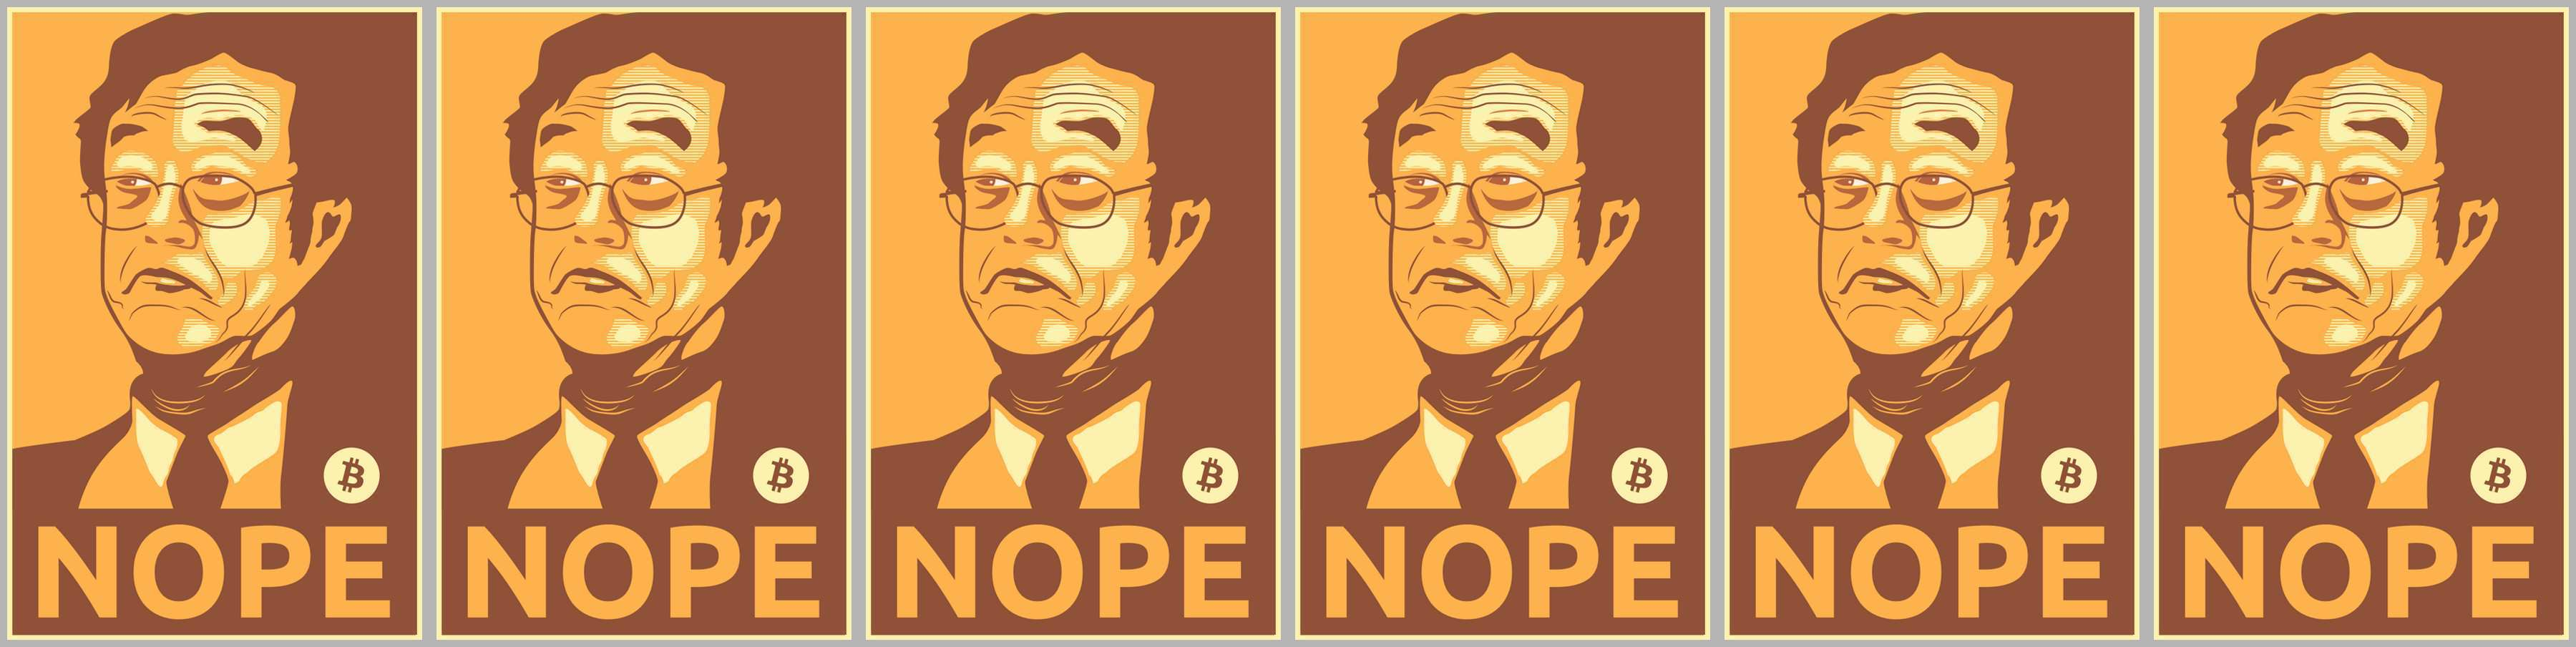
\includegraphics{assets/images/nope.png}
  \caption{Jeg er ikke Dorian Nakamoto.}
  \label{fig:nope}
\end{figure}

Uanset hvad hans virkelige identitet måtte være, havde Satoshi succes med at skjule den. Han satte et opmuntrende eksempel for alle, der ønsker at forblive anonyme: Det er muligt at have privatliv på internettet.\begin{quotation}\begin{samepage} \enquote{Kryptering virker. Korrekt implementerede, stærke kryptosystemer er en af de få ting, du kan stole på.} \begin{flushright} -- Edward Snowden\footnote{Edward Snowden, svarer på læsernes spørgsmål \cite{snowden}}
\end{flushright}\end{samepage}\end{quotation}

Satoshi var ikke den første pseudonyme eller anonyme opfinder, og han bliver heller ikke den sidste. Nogle har direkte efterlignet denne pseudonyme publikationsstil, blandt andre Tom Elvis Yedusor fra MimbleWimble~\cite{mimblewimble-origin} , mens andre har offentliggjort avancerede matematiske beviser, mens de har forblevet helt anonyme~\cite{4chan-math}.

Det er en mærkelig ny verden, vi lever i. En verden, hvor identitet er valgfri, og bidrag accepteres på baggrund af fortjeneste, samt hvor folk kan samarbejde og handle frit. Det vil kræve noget tilvænning at blive fortrolig med disse nye paradigmer, men jeg er overbevist om, at alt dette har potentialet til at ændre verden til det bedre.

Vi bør alle huske, at privatliv er en grundlæggende menneskerettighed\footnote{Verdenserklæringen om Menneskerettigheder, \textit{artikel 12}.~\cite{article12}}. Så længe folk udøver og forsvarer disse rettigheder, er kampen for privatlivets fred langt fra slut.\paragraph{Bitcoin har lært mig, at privatlivets fred ikke er død.}% ---
%
% #### Down the Rabbit Hole
%
% - [Universal Declaration of Human Rights][fundamental human right] by the United Nations
% - [A lower bound on the length of the shortest superpattern][anonymous] by Anonymous 4chan Poster, Robin Houston, Jay Pantone, and Vince Vatter
%
% [since the 80ies]: https://books.google.com/ngrams/graph?content=privacy+is+dead&year_start=1970&year_end=2019&corpus=15&smoothing=3&share=&direct_url=t1%3B%2Cprivacy%20is%20dead%3B%2Cc0
% [time-traveling AI]: https://blockchain24-7.com/is-crypto-creator-a-time-travelling-ai/
% ["I am not Dorian Nakamoto."]: http://p2pfoundation.ning.com/forum/topics/bitcoin-open-source?commentId=2003008%3AComment%3A52186
% [MimbleWimble]: https://github.com/mimblewimble/docs/wiki/MimbleWimble-Origin
% [anonymous]: https://oeis.org/A180632/a180632.pdf
% [fundamental human right]: http://www.un.org/en/universal-declaration-human-rights/
%
% <!-- Wikipedia -->
% [alice]: https://en.wikipedia.org/wiki/Alice%27s_Adventures_in_Wonderland
% [carroll]: https://en.wikipedia.org/wiki/Lewis_Carroll

\chapter{Cypherpunks skriver kode}
\label{les:20}

\begin{chapquote}{Lewis Carroll, \textit{Alice i Eventyrland}} \enquote{Jeg kan se, at du prøver at opfinde noget.} \end{chapquote}

Ligesom mange andre gode id\'eer, opstod Bitcoin ikke ud af ingenting. Det blev gjort muligt ved at benytte og kombinere mange innovationer og opdagelser inden for matematik, fysik, computervidenskab og andre områder. Satoshi var utvivlsomt et geni, men han ville ikke have været i stand til at opfinde Bitcoin uden de giganter, hvis skuldre han stod på.\begin{quotation}\begin{samepage} \enquote{Den, der kun ønsker og håber, blander sig ikke aktivt i begivenhedernes gang og i udformningen af sin egen skæbne.} \begin{flushright} -- Ludwig von Mises\footnote{Ludwig von Mises, \textit{Human Action} \cite{human-action}}
\end{flushright}\end{samepage}\end{quotation}% > <cite>[Ludwig Von Mises]</cite>

En af disse giganter er Eric Hughes, en af grundlæggerne af cypherpunk-bevægelsen og forfatter til \textit{A Cypherpunk's Manifesto}. Det er svært at forestille sig, at Satoshi ikke var påvirket af dette manifest. Det indbefatter mange ting, som Bitcoin muliggør og udnytter, såsom direkte og private transaktioner, elektroniske penge og kontanter, anonyme systemer og forsvar af privatlivets fred ved hjælp af kryptografi og digitale signaturer.\begin{quotation}\begin{samepage} \enquote{Privatliv er en nødvendighed for et åbent samfund i den elektroniske tidsalder. \href{...}{} Da vi ønsker privatlivets fred, må vi sikre, at hver part i en transaktion kun har kendskab til det, der er direkte nødvendigt for den pågældende transaktion. \href{...}{} Derfor kræver privatlivets fred i et åbent samfund anonyme transaktionssystemer. Indtil nu har kontanter været det primære system. Et anonymt transaktionssystem er ikke et hemmeligt transaktionssystem. \href{...}{} Vi Cypherpunks er dedikerede til at bygge anonyme systemer. Vi forsvarer vores privatliv med kryptografi, med anonyme systemer til videresendelse af e-mail, med digitale signaturer og med elektroniske penge. Cypherpunks skriver kode.} \begin{flushright} -- Eric Hughes\footnote{Eric Hughes, \textit{A Cypherpunk's Manifesto} \cite{cypherpunk-manifesto}}
\end{flushright}\end{samepage}\end{quotation}

Cypherpunks finder ikke trøst i håb og ønsker. De griber aktivt ind i begivenhedernes gang og former deres egen skæbne. Cypherpunks skriver kode.

På ægte cypherpunk-man\'er satte Satoshi sig derfor ned og begyndte at skrive kode. Denne kode tog en abstrakt id\'e og beviste overfor verden, at den faktisk virkede. Denne kode plantede frøet til en ny økonomisk virkelighed. Takket være denne kode kan alle bekræfte, at dette nye system rent faktisk fungerer, og hvert cirka 10. minut beviser Bitcoin over for verden, at den stadig er i live.\begin{figure}
  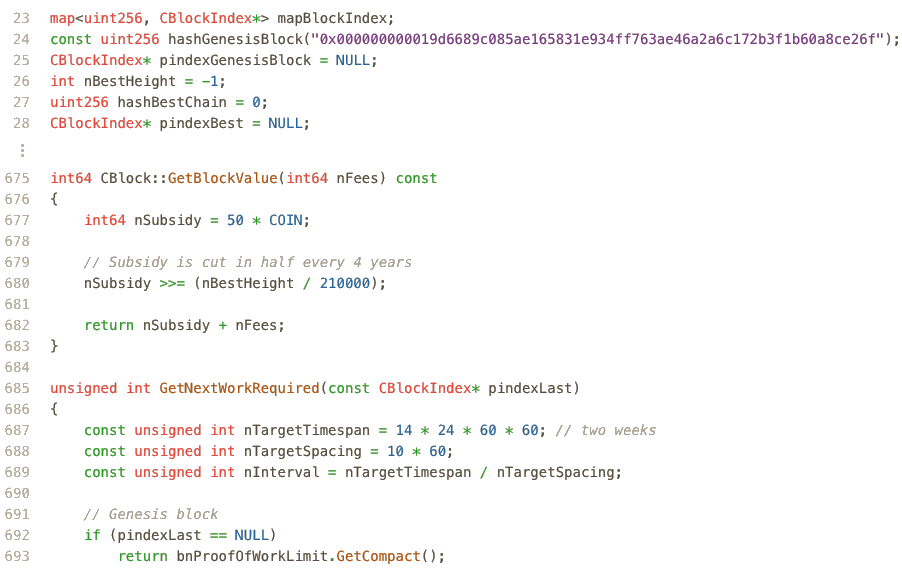
\includegraphics{assets/images/bitcoin-code-white.png}
  \caption{Kodeuddrag fra Bitcoin version 0.1}
  \label{fig:bitcoin-code-white}
\end{figure}

For at sikre, at hans innovation overgik fantasien og blev til virkelighed, skrev Satoshi koden til at implementere sin id\'e, før han skrev hvidbogen. Han sørgede også for ikke at forsinke\footnote{\enquote{Vi bør ikke udsætte for evigt, indtil hver eneste mulige funktionalitet er færdig.} - Satoshi Nakamoto~\cite{satoshi-delay}} udgivelsen for evigt. Når alt kommer til alt, \enquote{er der altid en ting mere at gøre.}\begin{quotation}\begin{samepage} \enquote{Jeg måtte skrive hele koden, før jeg kunne overbevise mig selv om, at jeg kunne løse alle problemerne. Derefter skrev jeg hvidbogen.} \begin{flushright} -- Satoshi Nakamoto\footnote{Satoshi Nakamoto, Re: Bitcoin P2P e-cash papir \cite{satoshi-mail-code-first}}
\end{flushright}\end{samepage}\end{quotation}

I nutidens verden af endeløse løfter og tvivlsom udførelse var der desperat brug for en udøvelse af dedikeret opbygning. Vær bevidst, overbevis dig selv om, at du faktisk kan løse problemerne, og implement\'er løsningerne. Vi bør alle stræbe efter at være lidt mere cypherpunk.\paragraph{Bitcoin har lært mig, at cypherpunks skriver kode.}% ---
%
% #### Down the Rabbit Hole
%
% - [Bitcoin version 0.1.0 announcement][version 0.1.0] by Satoshi Nakamoto
% - [Bitcoin P2P e-cash paper announcement][mail-announcement] by Satoshi Nakamoto
%
% [mail-announcement]: http://www.metzdowd.com/pipermail/cryptography/2008-October/014810.html
% [Ludwig Von Mises]: https://mises.org/library/human-action-0/html/pp/613
% [version 0.1.0]: https://bitcointalk.org/index.php?topic=68121.0
% [not to delay]: https://bitcointalk.org/index.php?topic=199.msg1670#msg1670
% [6]: http://www.metzdowd.com/pipermail/cryptography/2008-November/014832.html
%
% <!-- Wikipedia -->
% [alice]: https://en.wikipedia.org/wiki/Alice%27s_Adventures_in_Wonderland
% [carroll]: https://en.wikipedia.org/wiki/Lewis_Carroll

\chapter{Metaforer for Bitcoins fremtid}
\label{les:21}

\begin{chapquote}{Lewis Carroll, \textit{Alice i Eventyrland}}
\enquote{Jeg ved, at der helt sikkert vil ske noget interessant\ldots}
\end{chapquote}

I de sidste par årtier er det tydeligt, at teknologisk innovation ikke følger en lineær trend. Uanset om man tror på den teknologiske singularitet eller ej, er det ubestrideligt, at fremskridtene på mange områder er eksponentielle. Ikke alene det, men hastigheden, hvormed teknologier bliver taget i brug, accelererer også. Før du ved af det, er busken i den lokale skolegård væk, og dine børn bruger Snapchat i stedet. Eksponentielle kurver har en tendens til at give dig en forskrækkelse, længe før du ser dem komme.

Bitcoin er en eksponentiel teknologi, der bygger på eksponentielle teknologier. \textit{Our World in Data}\footnote{\url{https://ourworldindata.org/}} viser smukt den stigende hastighed af teknologisk adoption, startende i 1903 med introduktionen af fastnettelefoner (se Figur~\ref{fig:tech-adoption}). Fastnettelefoner, elektricitet, computere, internettet og smartphones følger alle eksponentielle tendenser i pris, ydeevne og udbredelse. Bitcoin gør også dette~\cite{tech-adoption}.

\begin{figure}
  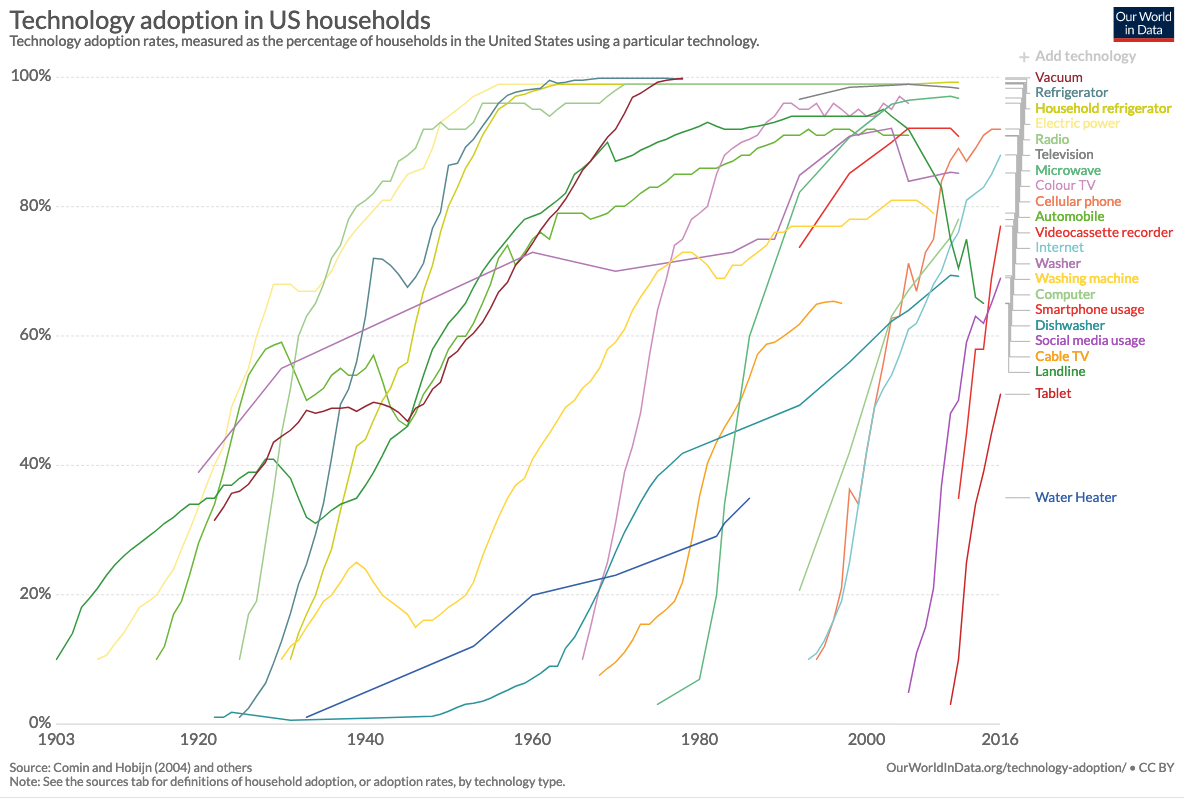
\includegraphics{assets/images/tech-adoption.png}
  \caption{Bitcoin er bogstaveligt talt helt uden for skalaen.}
  \label{fig:tech-adoption}
\end{figure}

Bitcoin har ikke kun \'en, men flere netværkseffekter\footnote{Trace Mayer, \textit{The Seven Network Effects of Bitcoin}~\cite{7-network-effects}}, som alle resulterer i eksponentielle vækstmønstre inden for deres respektive områder: pris, brugere, sikkerhed, udviklere, markedsandel og anvendelse som globale penge.

Efter at have overlevet sin spæde begyndelse fortsætter Bitcoin med at vokse hver dag i mere end \'et aspekt. Indrømmet, teknologien har ikke nået sin modenhed endnu. Den befinder sig måske i ungdomsårene. Men hvis teknologien er eksponentiel, er vejen fra ubemærkethed til allestedsnærværende kort.\begin{figure}
  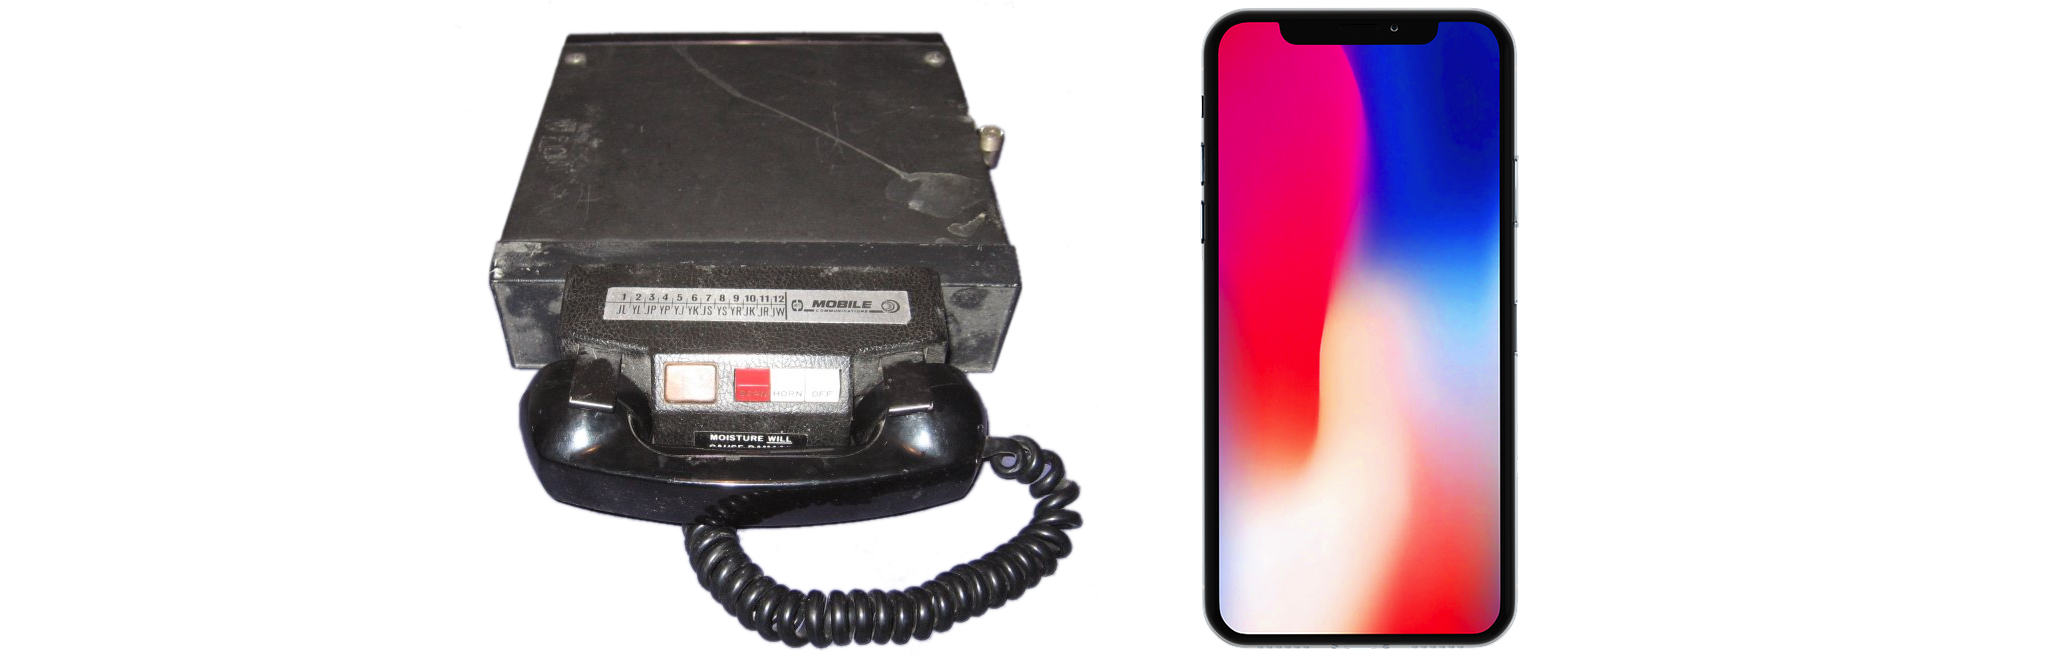
\includegraphics{assets/images/mobile-phone.png}
  \caption{Mobiltelefon, ca. 1965 vs. 2019.}
  \label{fig:mobile-phone}
\end{figure}

I sin TED Talk fra 2003 valgte Jeff Bezos at bruge elektricitet som en metafor for nettets fremtid.\footnote{\url{http://bit.ly/bezos-web}} Alle tre fænomener - elektricitet, internettet og Bitcoin - er \textit{aktiverende} netværksteknologier, der muliggør andre ting. De er infrastrukturer, der skal bygges ovenpå, og deres natur er at være grundlaget for andre teknologier.

Elektricitet har eksisteret i lang tid nu. Vi tager den for givet. Internettet er betydeligt yngre, men de fleste tager det også for givet. Bitcoin er ti år gammel og er trængt ind i den offentlige bevidsthed under den sidste hype-cyklus. Kun de tidligste brugere tager den for givet. Som tiden går, vil flere og flere mennesker anerkende Bitcoin som noget, der bare er.\footnote{Dette er kendt som \textit{Lindy-effekten}. Lindy-effekten er en teori om, at den fremtidige forventede levetid for ikke-forgængelige fænomener som en teknologi eller en id\'e er proportional med deres nuværende alder, således at hver ekstra periode med overlevelse indikerer en længere forventet restlevetid.~\cite{wiki:lindy}}

I 1994 var internettet stadig forvirrende og det var ikke intuitivt. Når man ser denne gamle optagelse af \textit{Today Show}\footnote{\url{https://youtu.be/UlJkuSyNg_C}} bliver det tydeligt, at det, der føles naturligt og intuitivt nu, faktisk ikke var det dengang. Bitcoin er stadig forvirrende og fremmed for de fleste, men ligesom internettet er naturligt for den digitalt indfødte, vil det at bruge og stable sats\footnote{\url{https://twitter.com/hashtag/stackingsats}} være en selvfølge for fremtidens bitcoin-indfødte.\begin{quotation}\begin{samepage} \enquote{Fremtiden er allerede her - den er bare ikke jævnt fordelt.} \begin{flushright} -- William Gibson\footnote{William Gibson, \textit{The Science in Science Fiction} \cite{william-gibson}}
\end{flushright}\end{samepage}\end{quotation}

I 1995 brugte omkring $15\%$ af voksne amerikanere internettet. Historiske data fra Pew Research Center~\cite{pew-research} viser, hvordan internettet har vævet sig ind i alle vores liv. Ifølge en forbrugerundersøgelse foretaget af Kaspersky Lab~\cite{web:kaspersky}, har $13\%$ af de adspurgte brugt Bitcoin og dens kloner til at betale for varer i 2018. Selvom betalinger ikke er det eneste anvendelsesområde for bitcoin, er det en indikation af, hvor vi befinder os i internettid: Vi er i begyndelsen til midten af 90'erne.

I 1997 udtalte Jeff Bezos i et brev til aktionærerne~\cite{bezos-letter} at \enquote{Dette er dag 1 for internettet}, og han erkendte det store uudnyttede potentiale for både internettet og sin virksomhed. Uanset hvilken dag det er for Bitcoin, er de enorme mængder uudnyttet potentiale tydelige for alle, undtagen den mest dovne iagttager.\begin{figure}
  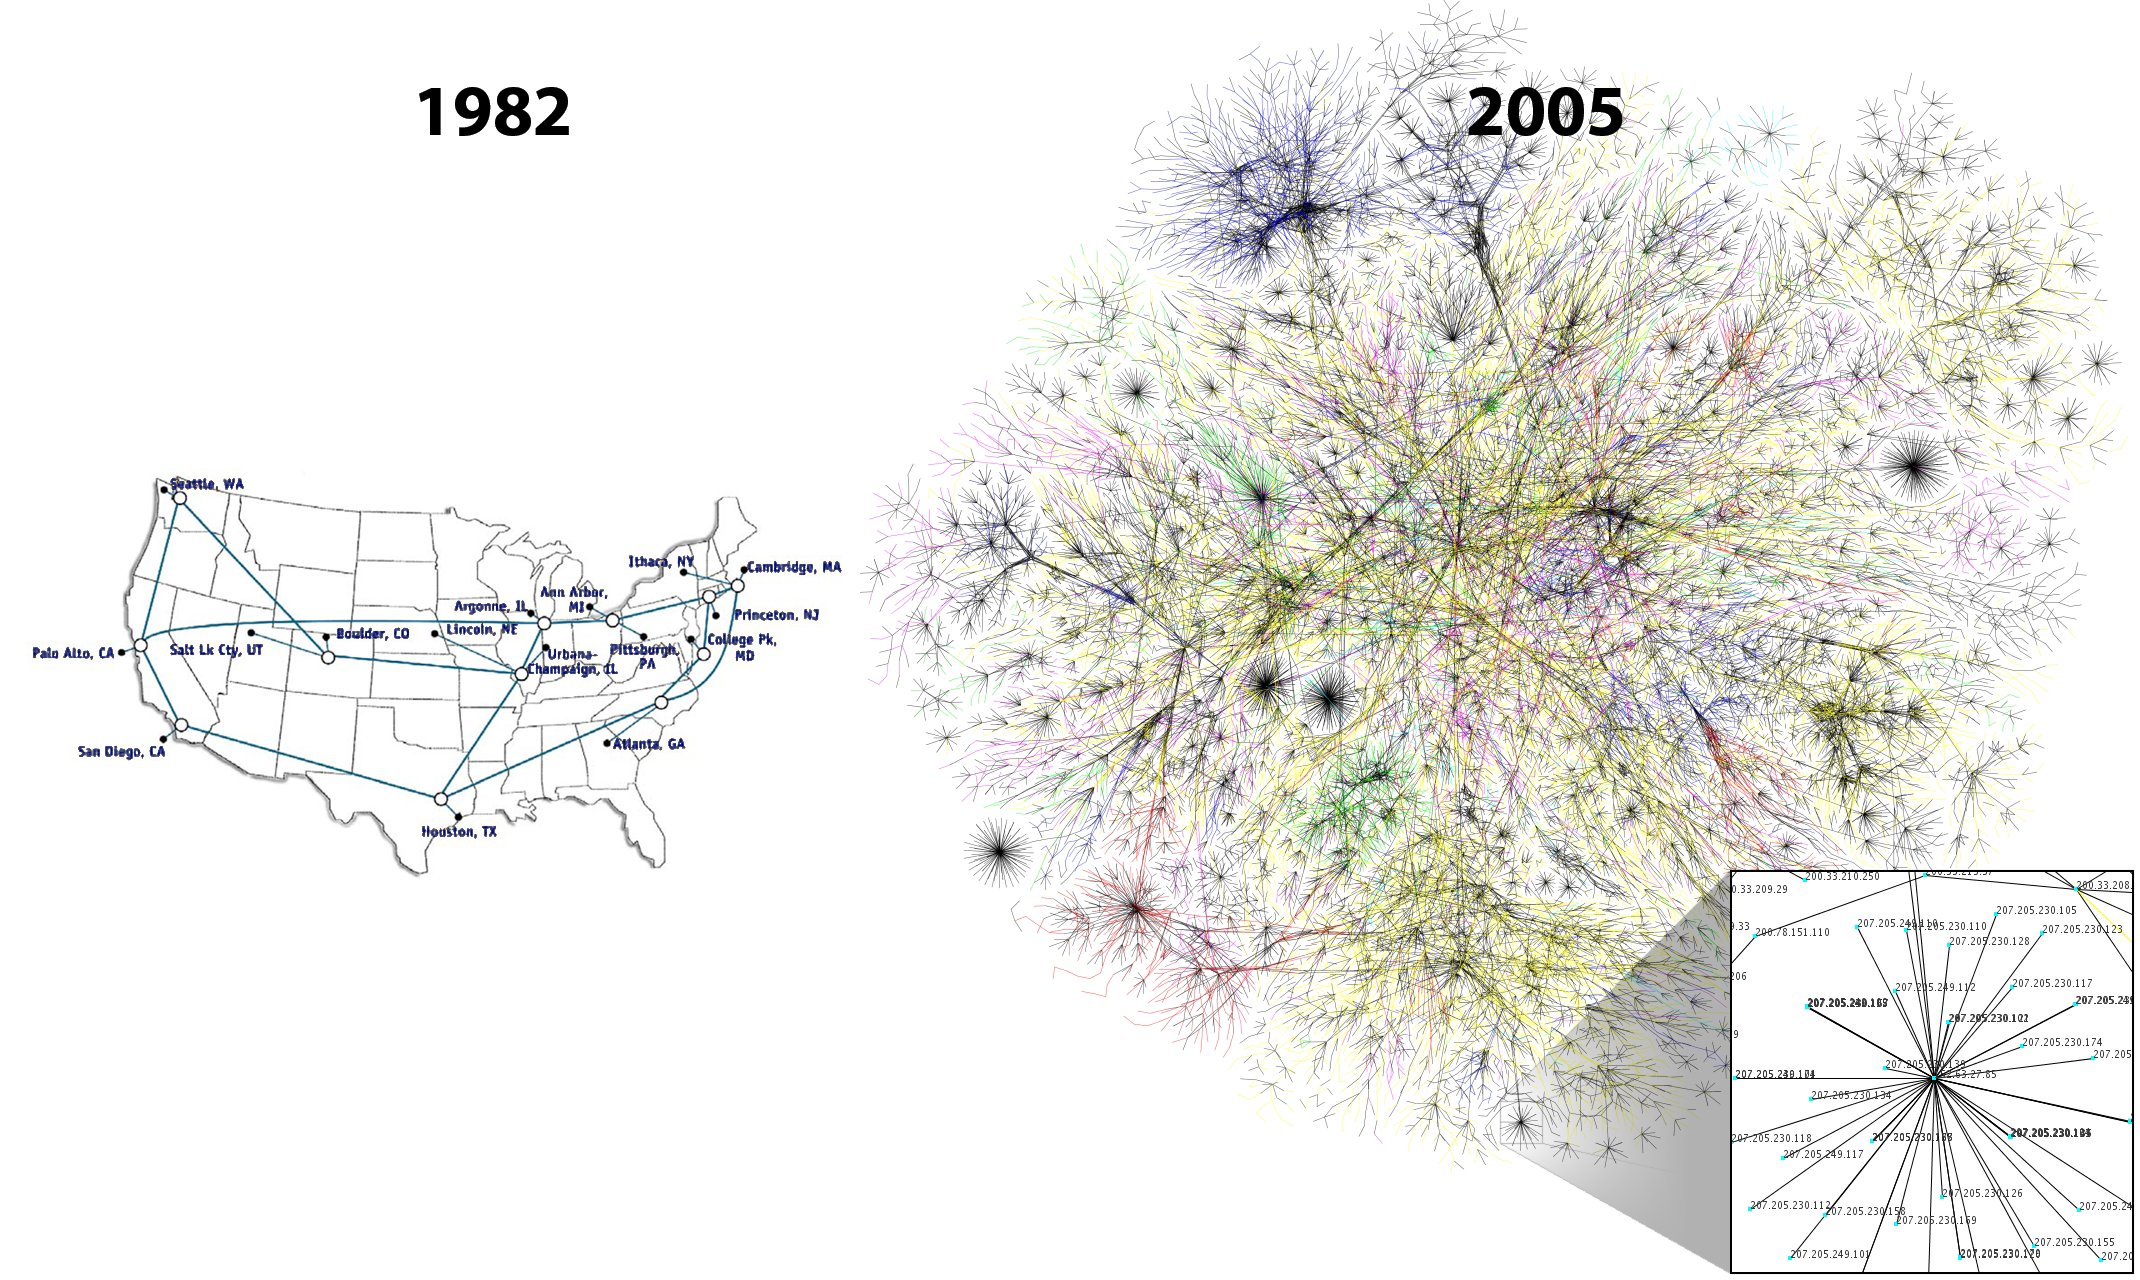
\includegraphics{assets/images/internet-evolution-white-dates.png}
  \caption{Internettet, 1982 vs 2005. Kilde: cc-by Merit Network, Inc. og Barrett Lyon, Opte Project}
  \label{fig:internet-evolution-white-dates}
\end{figure}

Bitcoins første knudepunkt kom online i 2009, efter at Satoshi havde udvundet \textit{skabelses-blokken}\footnote{Skabelses-blokken er den første blok i Bitcoins blokkæde. Moderne versioner af Bitcoin tæller den som blok $0$, selvom tidlige versioner talte den som blok $1$. Skabelses-blokken er normalt inkluderet i softwaren til de applikationer, der bruger Bitcoin-blokkæden. Den er speciel, fordi den ikke refererer til en tidligere blok og producerede en blokbelønning, der ikke kan bruges. Parameteren \textit{coinbase} indeholder, sammen med de normale data, følgende tekst: \textit{\enquote{The Times 03/Jan/2009 Kansler på randen af anden redningspakke til bankerne}} \cite{btcwiki:genesis-block}} og frigav softwaren ud i naturen. Hans knudepunkt var ikke alene længe. Hal Finney var en af de første, der forstod ideen og han sluttede sig til netværket. Ti år senere, da dette skrives, kører mere end $75.000$\footnote{\url{https://bit.ly/luke-nodecount}} knudepunkter Bitcoin.\begin{figure}
  \centering
  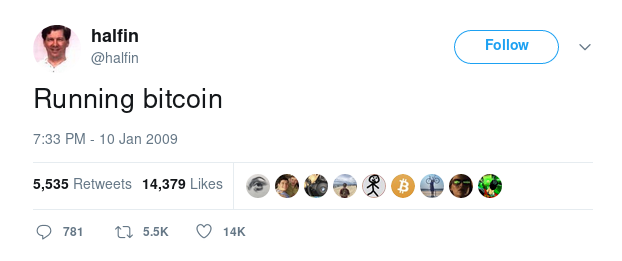
\includegraphics[width=8cm]{assets/images/running-bitcoin.png}
  \caption{Hal Finney skrev det første tweet, der nævnte bitcoin, i januar 2009.}
  \label{fig:running-bitcoin}
\end{figure}

Protokollens basislag er ikke det eneste, der vokser eksponentielt. Lightning-netværket, en teknologi der bygger ovenpå Bitcoin, vokser endnu hurtigere.

I januar 2018 havde Lightning-netværket $40$ knudepunkter og $60$ kanaler~\cite{web:lightning-nodes}. I april 2019 var netværket vokset til mere end $4.000$ knudepunkter og omkring $40.000$ kanaler. Husk på, at dette stadig er en eksperimentel teknologi, hvor tab af midler kan ske og sker. Men tendensen er klar: Tusindvis af mennesker er hensynsløse og ivrige efter at bruge det.\begin{figure}
  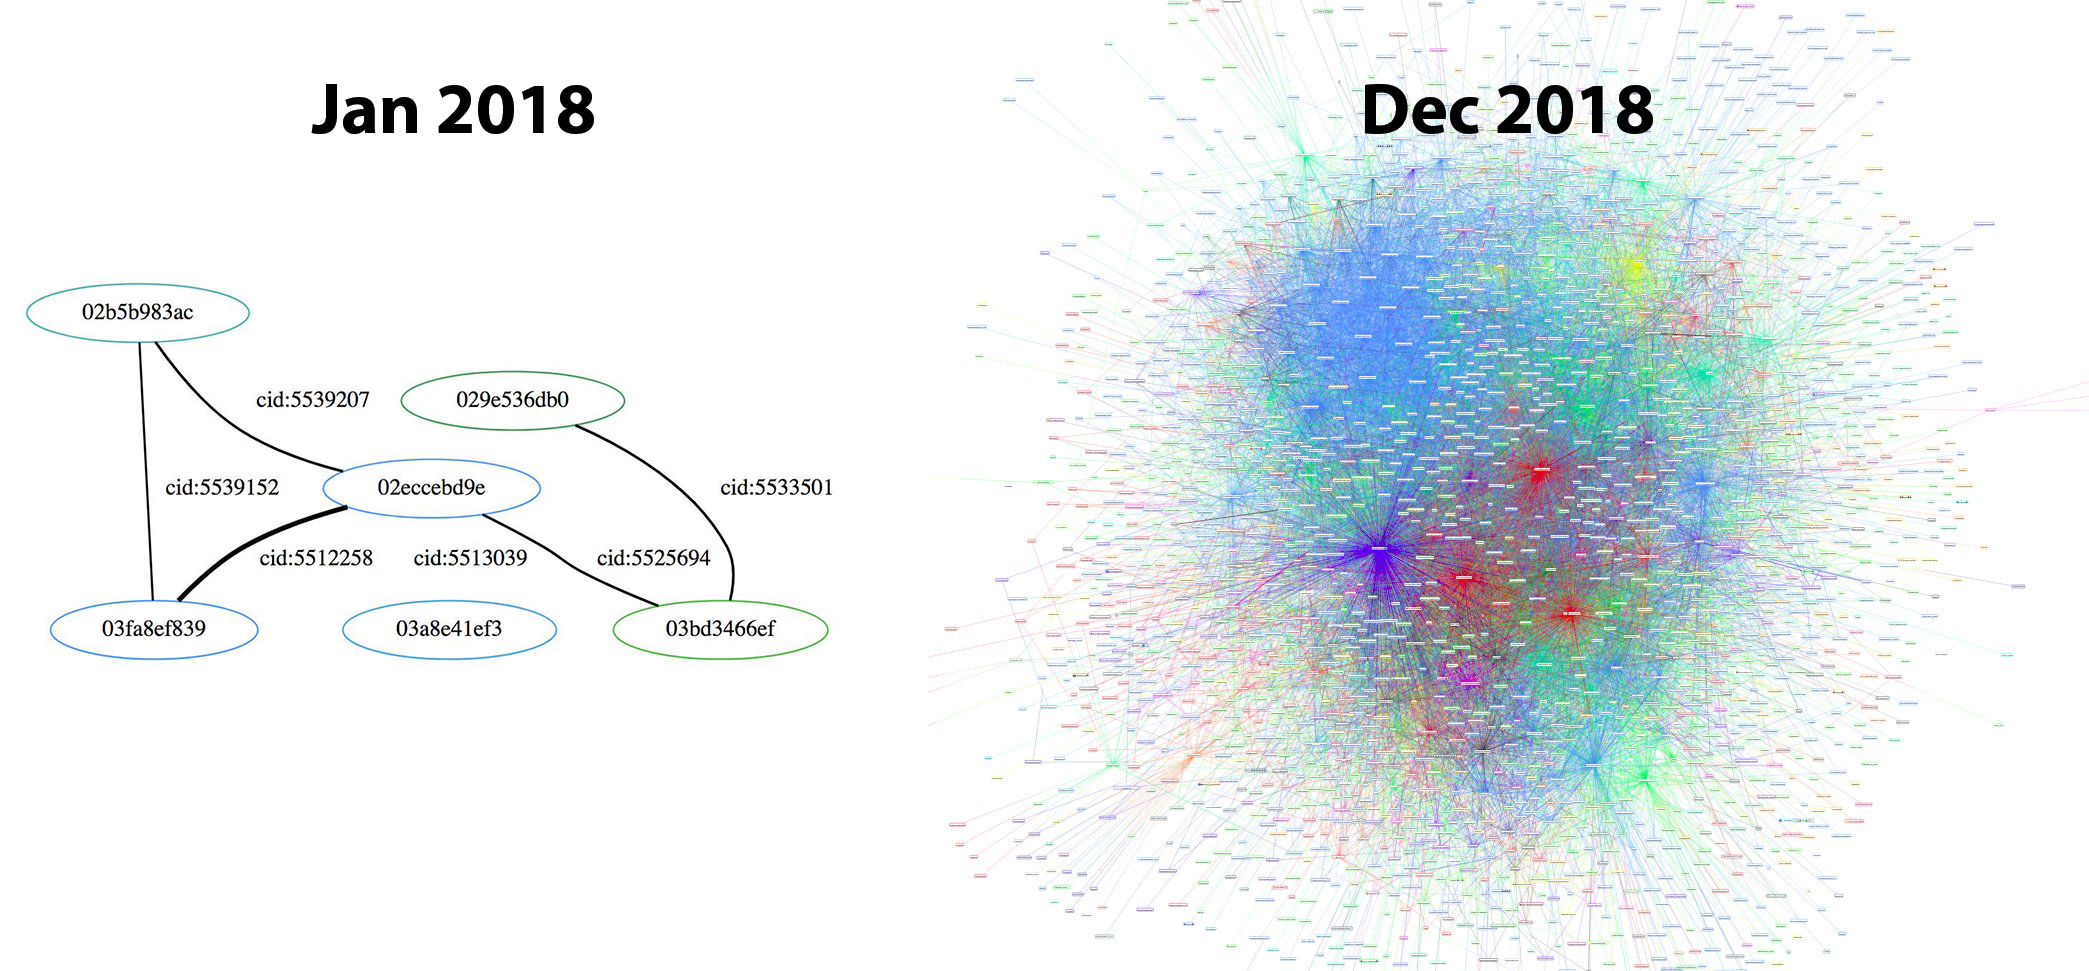
\includegraphics{assets/images/lnd-growth-lopp-white.png}
  \caption{Lightning-netværket, januar 2018 vs. december 2018. Kilde: Jameson Lopp}
  \label{fig:lnd-growth-lopp-white.png}
\end{figure}

For mig, der har oplevet internettets meteoriske fremgang, er parallellerne mellem internettet og Bitcoin åbenlyse. Begge er netværk, begge er eksponentielle teknologier, og begge skaber nye muligheder, nye industrier og nye måder at leve på. Ligesom elektricitet var den bedste metafor til at forstå, hvor internettet er på vej hen, kan internettet være den bedste metafor til at forstå, hvor bitcoin er på vej hen. Eller, som Andreas Antonopoulos siger, Bitcoin er \textit{pengenes internet}. Disse metaforer er en god påmindelse om, at selvom historien ikke gentager sig selv, så rimer den ofte.

Eksponentielle teknologier er svære at forstå og bliver ofte undervurderede. Selvom jeg har en stor interesse i sådanne teknologier, bliver jeg konstant overrasket over tempoet i fremskridt og innovation. At se Bitcoin-økosystemet vokse er som at se en hurtigspolet optagelse af internettets opståen. Det er fantastisk opløftende.

Min søgen efter at forstå Bitcoin har ført mig ned ad historiens stier på mere end \'en måde. At forstå gamle samfundsstrukturer, fortidens penge, og hvordan kommunikationsnetværk udviklede sig, var alt sammen en del af rejsen. Fra håndøksen til smartphonen har teknologien utvivlsomt ændret vores verden mange gange. Netværksteknologier er særligt transformerende: skrift, veje, elektricitet og internettet. De har alle ændret verden. Bitcoin har ændret min verden og vil fortsætte med at ændre tankerne og hjerterne hos dem, der tør bruge den.\paragraph{Bitcoin har lært mig, at det er vigtigt at forstå fortiden for at forstå dens fremtid. En fremtid, som kun lige er begyndt\ldots}% ---
%
% #### Down the Rabbit Hole
%
% - [The Rising Speed of Technological Adoption][the rising speed of technological adoption] by Jeff Desjardins
% - [The 7 Network Effects of Bitcoin][multiple network effects] by Trace Mayer
% - [The Electricity Metaphor for the Web's Future][TED talk] by Jeff Bezos
% - [How the internet has woven itself into American life][data from the Pew Research Center] by Susannah Fox and Lee Rainie
% - [Genesis Block][genesis block] on the Bitcoin Wiki
% - [Lindy Effect][more time] on Wikipedia
%
% [Our World in Data]: https://ourworldindata.org/
% [the rising speed of technological adoption]: https://www.visualcapitalist.com/rising-speed-technological-adoption/
% [multiple network effects]: https://www.thrivenotes.com/the-7-network-effects-of-bitcoin/
% [TED talk]: https://www.ted.com/talks/jeff_bezos_on_the_next_web_innovation
% [recording of the Today Show]: https://www.youtube.com/watch?v=UlJku_CSyNg
% [William Gibson]: https://www.npr.org/2018/10/22/1067220/the-science-in-science-fiction
% [data from the Pew Research Center]: https://www.pewinternet.org/2014/02/27/part-1-how-the-internet-has-woven-itself-into-american-life/
% [consumer survey]: https://www.kaspersky.com/blog/money-report-2018/
% [letter to shareholders]: http://media.corporate-ir.net/media_files/irol/97/97664/reports/Shareholderletter97.pdf
% [running bitcoin]: https://twitter.com/halfin/status/1110302988?lang=en
% [40 nodes]: https://bitcoinist.com/bitcoin-lightning-network-mainnet-nodes/
% [reckless]: https://twitter.com/hashtag/reckless
% [Jameson Lopp]: https://twitter.com/lopp/status/1077200836072296449
% [\textit{The Internet of Money}]: https://theinternetofmoney.info/
% [stacking]: https://twitter.com/hashtag/stackingsats
%
% <!-- Bitcoin Wiki -->
% [genesis block]: https://en.bitcoin.it/wiki/Genesis_block
%
% <!-- Wikipedia -->
% [more time]: https://en.wikipedia.org/wiki/Lindy_effect
% [alice]: https://en.wikipedia.org/wiki/Alice%27s_Adventures_in_Wonderland
% [carroll]: https://en.wikipedia.org/wiki/Lewis_Carroll

\addpart{Afsluttende tanker}
\pdfbookmark{Conclusion}{conclusion}
\label{ch:conclusion}

\chapter*{Konklusion}

\begin{chapquote}{Lewis Carroll, \textit{Alice i Eventyrland}} \enquote{Begynd ved begyndelsen,} sagde kongen alvorligt, \enquote{og fortsæt, indtil du kommer til slutningen. Og hold så op.} \end{chapquote}

Som nævnt i begyndelsen tror jeg, at ethvert svar på spørgsmålet \textit{\enquote{Hvad har du lært af Bitcoin?}} altid vil være ufuldstændigt. Symbiosen af hvad der kan ses som flere levende systemer - Bitcoin, teknosfæren og økonomi - er for indviklet, emnerne for mange, og tingene bevæger sig for hurtigt til nogensinde at blive fuldt ud forstået af en enkelt person.

Selv uden at forstå det fuldt ud, og til trods for alle dets særheder og tilsyneladende mangler, fungerer Bitcoin utvivlsomt. Den bliver ved med at producere blokke cirka hvert tiende minut, og den gør det på en smuk måde. Jo længere Bitcoin fortsætter med at fungere, des flere mennesker vil vælge at bruge den.\begin{quotation}\begin{samepage} \enquote{Det er sandt, at ting er smukke, når de fungerer. Kunst er funktion.} \begin{flushright} -- Giannina Braschi\footnote{Giannina Braschi, \textit{Empire of Dreams} \cite{braschi2011empire}}
\end{flushright}\end{samepage}\end{quotation}

\paragraph{} Bitcoin er født af internettet. Den vokser eksponentielt og udvisker grænserne mellem discipliner. Det er for eksempel ikke klart, hvor teknologiens verden ender, og hvor en anden verden begynder. Selvom Bitcoin kræver computere for at fungere effektivt, er datalogi ikke tilstrækkeligt for at forstå den. Bitcoin er ikke kun grænseløs med hensyn til sin indre funktion, men også grænseløs i forhold til akademiske discipliner.

Økonomi, politik, spilteori, monetær historie, netværksteori, finansiering, kryptografi, informationsteori, censur, lovgivning og regulering, menneskelig organisation og psykologi - alle disse og mange flere er ekspertiseområder, der kan bidrage til forståelsen af, hvordan Bitcoin fungerer, og hvad Bitcoin er.

Ingen enkeltstående opfindelse er ansvarlig for dens succes. Det er kombinationen af flere tidligere uafhængige brikker, sat sammen af spilteoretiske incitamenter, der udgør den revolution, som Bitcoin er. Den smukke blanding af mange discipliner er det, der gør Satoshi til et geni.\paragraph{} Som ethvert komplekst system skal Bitcoin foretage afvejninger mellem effektivitet, omkostninger, sikkerhed og mange andre egenskaber. Ligesom der ikke er nogen perfekt løsning på at udlede en firkant fra en cirkel, vil enhver løsning på de problemer, som Bitcoin forsøger at løse, også altid være ufuldkommen.\begin{quotation}\begin{samepage} \enquote{Jeg tror ikke, at vi nogensinde vil få gode penge igen, før vi tager dem ud af statens hænder. Det vil sige, vi kan ikke tage dem ud af statens hænder med vold; det eneste vi kan gøre er at indføre noget via snedige, indirekte bagveje, som de ikke kan stoppe.} \begin{flushright} -- Friedrich Hayek\footnote{Friedrich Hayek on Monetary Policy, the Gold Standard, Deficits, Inflation, and John Maynard Keynes \url{https://youtu.be/EYhEDxFwFRU}}
\end{flushright}\end{samepage}\end{quotation}

Bitcoin er den snedige, indirekte bagvej som de ikke kan stoppe, og er dermed måden, hvorpå man kan genintroducere verden til gode penge. Den skaber et suverænt individ bag hvert knudepunkt, ligesom Da Vinci forsøgte at løse det uløselige problem med at kvadrere en cirkel ved at placere den vitruvianske mand i cirklens centrum. Knudepunkter fjerner effektivt ethvert koncept om et centrum og skaber et system, som er forbløffende anti-skrøbeligt og ekstremt svært at lukke ned. Bitcoin lever, og dens hjerteslag vil sandsynligvis overleve os alle.

Jeg håber, du har nydt disse 21 lektioner. Måske er den vigtigste lektion, at man bør undersøge Bitcoin holistisk og fra flere vinkler, hvis man gerne vil have noget, der minder om et komplet billede. Ligesom det at fjerne en del fra et komplekst system ødelægger helheden, synes det at ødelægge forståelsen af Bitcoin at undersøge dele af den i isolation. Hvis bare \'en person fjerner \enquote{blokkæden} fra sit ordforråd og erstatter det med \enquote{en kæde af blokke}, vil jeg dø som en lykkelig mand.

Under alle omstændigheder fortsætter min rejse. Jeg planlægger at vove mig længere ned i kaninhullets dybder, og jeg inviterer dig til at tage med på turen.\footnote{\url{https://twitter.com/dergigi}}% <!-- Twitter -->
% [dergigi]: https://twitter.com/dergigi
%
% <!-- Internal -->
% [sly roundabout way]: https://youtu.be/EYhEDxFwFRU?t=1124
% [Giannina Braschi]: https://en.wikipedia.org/wiki/Braschi%27s_Empire_of_Dreams

\cleardoublepage

\chapter*{Takkeord}
\pdfbookmark{Acknowledgments}{acknowledgments}

Tak til de utallige forfattere og indholdsproducenter, der har påvirket min tankegang om Bitcoin og de emner, den berører. Der er for mange til at nævne dem alle, men jeg vil gøre mit bedste for at nævne nogle få.\begin{itemize}
  \item Tak til Arjun Balaji for tweeten, der motiverede mig til at skrive dette. \item Tak til Marty Bent for at give endeløs stof til eftertanke og underholdning. Hvis du ikke abonnerer på \textit{Marty's Bent} og \textit{Tales From The Crypt}, er du gået glip af noget. Skål for Matt og Marty der guider os gennem kaninhullet. \item Tak til Michael Goldstein og Pierre Rochard for udvælgelsen af materiale og levering af den bedste Bitcoin-litteratur via Nakamoto Institute. Og tak for skabelsen af Noded Podcast, som i høj grad har påvirket mit filosofiske syn på Bitcoin. \item Tak til Saifedean Ammous for hans overbevisninger, nådesløse tweets og for at have skrevet Bitcoinstandarden \item Tak til Francis Pouliot for at dele sin begejstring over at opdage tidskæden. \item Tak til Andreas M. Antonopoulos for alt det uddannelsesmateriale, han har udgivet i årenes løb. \item Tak til Peter McCormack for hans ærlige tweets og podcasten \textit{What Bitcoin Did}, som fortsat leverer fantastiske indsigter fra mange områder inden for feltet. \item Tak til Jannik, Brandon, Matt, Camilo, Daniel, Michael, og Raphael for at give feedback på de tidlige udkast til nogle lektioner. En særlig tak til Jannik, der korrekturlæste flere udkast flere gange. \item Tak til Dhruv Bansal og Matt Odell for at tage sig tid til at diskutere nogle af disse ideer med mig. \item Tak til Guy Swann for at producere en lydversion af 21lessons.com. \item Tak til Friar Hass for hans åndelige støtte og vejledning, og for at tage sig tid til at skrive et forord til denne bog. \item Tak til min kone for at holde mig og min besættelse ud. \item Tak til min familie for at støtte mig i både gode og dårlige tider. \item Sidst, men ikke mindst, tak til alle bitcoin-maksimalister, shitcoin-minimalister, shills, bots og shitposters, som holder til i den smukke have, som Bitcoin Twitter er. \end{itemize}

Og til sidst, tak fordi du læste dette. Jeg håber, du nød det lige så meget, som jeg nød at skrive det. 

\listoffigures

\chapter*{Om bibliografien}
\pdfbookmark{Bibliography}{bibliography}

I dag er der udgivet mange af bøger om Bitcoin. Men det meste af samtalen - og dermed de fleste af de interessante ressourcer - findes online.\paragraph{} Denne bibliografi inkluderer en række bøger, artikler og online-ressourcer. Hvis ressourcen har en tilknyttet URL, var denne aktiv i oktober 2019, hvor jeg havde adgang til den pågældende ressource. Hvis en af de følgende URL'er fører til en død side, beklager jeg. Lad mig venligst vide det\footnote{\url{https://dergigi.com/contact}} så jeg kan opdatere linket/linkene.\paragraph{} P.S.: Bitcoin og \href{https://ipfs.io/}{IPFS} løser det. 
\bibliography{main}
\part{Den danske version}

Denne danske version af 21 Lektioner er blevet oversat af et team af
danske Bitcoin-entusiaster, der er passionerede om at sprede budskabet
om Bitcoin og dens potentiale til at forbedre verden.

Vi håber, at du har nydt at læse 21 Lessons og at du vil være med til at
sprede budskabet.

\section*{Motivation}

Vi har oversat 21 Lektioner til dansk, da vi tror på, at den tilbyder en
lettilgængelig introduktion til Bitcoin og dens principper. I modsætning
til mange andre bøger om Bitcoin dækker 21 Lektioner et bredt spektrum
af de elementer, der gør Bitcoin til Bitcoin. Den er kortfattet, skrevet
på et letforståeligt dansk og med et begrænset brug af teknisk jargon.
Vi har alle startet samme sted, hvor vi kigger på den hvide kanin, der
hopper af sted, og som i Alice i Eventyrland så starter rejsen hvor
Alice hopper ned i kaninhullet uden at tænke på hvorfor en kanin har et
lommeur og vest. Eventyret ville dog have været anderledes, hvis Alice
havde haft en rejseberetning med skrevet af Bob eller Gigi.
\newpage
\section*{Handling:}

Vi opfordrer dig til at lære mere om Bitcoin og blive involveret i
Bitcoin-fællesskabet. Du kan finde mere information på følgende
ressourcer:

\begin{itemize}
\item
  \begin{quote}
  Telegram-kanalen "EnOgTyve":
  \href{https://t.me/enogtyvedk}{https://t.me/enogtyvedk}
  \end{quote}
\item
  \begin{quote}
  Dansk Platform -
  \href{https://www.enogtyve.org/}{https://www.enogtyve.org}
  \end{quote}
\item
  \begin{quote}
  Bogen `Bitcoin Standarden:
  \href{https://www.bitcoinstandarden.dk/}{https://www.bitcoinstandarden.dk}
  \end{quote}
\item
  \begin{quote}
  Bitcoinskolen.net:
  \href{https://www.bitcoinskolen.net/}{https://www.bitcoinskolen.net/}
  \end{quote}
\end{itemize}

\section*{Taknemmelighed:}

Teamet vil gerne takke følgende personer for deres bidrag til
oversættelsen og korrekturlæsning:

\begin{itemize}
\item
  \begin{quote}
  Peter Isaksen
  \end{quote}
\item
  \begin{quote}
  Rasmus Hansen
  \end{quote}
\item
  \begin{quote}
  Pierre Vendelbo
  \end{quote}
\item
  \begin{quote}
  Btcblot
  \end{quote}
\item
  \begin{quote}
  Rune Kristensen
  \end{quote}
\end{itemize}

\textbf{Følg den hvide kanin!}

\end{document}
